% Options for packages loaded elsewhere
\PassOptionsToPackage{unicode}{hyperref}
\PassOptionsToPackage{hyphens}{url}
%
\documentclass[
]{book}
\usepackage{lmodern}
\usepackage{amssymb,amsmath}
\usepackage{ifxetex,ifluatex}
\ifnum 0\ifxetex 1\fi\ifluatex 1\fi=0 % if pdftex
  \usepackage[T1]{fontenc}
  \usepackage[utf8]{inputenc}
  \usepackage{textcomp} % provide euro and other symbols
\else % if luatex or xetex
  \usepackage{unicode-math}
  \defaultfontfeatures{Scale=MatchLowercase}
  \defaultfontfeatures[\rmfamily]{Ligatures=TeX,Scale=1}
\fi
% Use upquote if available, for straight quotes in verbatim environments
\IfFileExists{upquote.sty}{\usepackage{upquote}}{}
\IfFileExists{microtype.sty}{% use microtype if available
  \usepackage[]{microtype}
  \UseMicrotypeSet[protrusion]{basicmath} % disable protrusion for tt fonts
}{}
\makeatletter
\@ifundefined{KOMAClassName}{% if non-KOMA class
  \IfFileExists{parskip.sty}{%
    \usepackage{parskip}
  }{% else
    \setlength{\parindent}{0pt}
    \setlength{\parskip}{6pt plus 2pt minus 1pt}}
}{% if KOMA class
  \KOMAoptions{parskip=half}}
\makeatother
\usepackage{xcolor}
\IfFileExists{xurl.sty}{\usepackage{xurl}}{} % add URL line breaks if available
\IfFileExists{bookmark.sty}{\usepackage{bookmark}}{\usepackage{hyperref}}
\hypersetup{
  pdftitle={Theoretical and empirical investigation of echolocation in bat groups},
  pdfauthor={Thejasvi Beleyur},
  hidelinks,
  pdfcreator={LaTeX via pandoc}}
\urlstyle{same} % disable monospaced font for URLs
\usepackage{longtable,booktabs}
% Correct order of tables after \paragraph or \subparagraph
\usepackage{etoolbox}
\makeatletter
\patchcmd\longtable{\par}{\if@noskipsec\mbox{}\fi\par}{}{}
\makeatother
% Allow footnotes in longtable head/foot
\IfFileExists{footnotehyper.sty}{\usepackage{footnotehyper}}{\usepackage{footnote}}
\makesavenoteenv{longtable}
\usepackage{graphicx,grffile}
\makeatletter
\def\maxwidth{\ifdim\Gin@nat@width>\linewidth\linewidth\else\Gin@nat@width\fi}
\def\maxheight{\ifdim\Gin@nat@height>\textheight\textheight\else\Gin@nat@height\fi}
\makeatother
% Scale images if necessary, so that they will not overflow the page
% margins by default, and it is still possible to overwrite the defaults
% using explicit options in \includegraphics[width, height, ...]{}
\setkeys{Gin}{width=\maxwidth,height=\maxheight,keepaspectratio}
% Set default figure placement to htbp
\makeatletter
\def\fps@figure{htbp}
\makeatother
\setlength{\emergencystretch}{3em} % prevent overfull lines
\providecommand{\tightlist}{%
  \setlength{\itemsep}{0pt}\setlength{\parskip}{0pt}}
\setcounter{secnumdepth}{5}
\usepackage{booktabs}
\usepackage{caption}
\usepackage{graphicx}
\usepackage{lscape}
\usepackage{booktabs}
\usepackage{caption}
\captionsetup{font=footnotesize}
\usepackage{tabu}
\usepackage{amsmath,amssymb,graphicx,todonotes}
\usepackage{url}
\usepackage{booktabs}
\usepackage{algorithm}
\usepackage{algpseudocode}
\usepackage{epstopdf}

\def\x{{\mathbf x}}
\def\L{{\cal L}}
\def\lone{{$l^1$}}
\def\ltwo{{$l^2$}}
\def \fatR {{ \mathbb R}}
\DeclareMathOperator{\Tr}{Tr}
\providecommand{\norm}[1]{\lVert#1\rVert}
\newtheorem{problem1}{\noindent \textbf{Problem}}
\newtheorem{theorem}{\noindent \textbf{Theorem}}
\newtheorem{algorithm1}{\noindent \textbf{Algorithm}}
\newtheorem{lemma}{\noindent \textbf{Lemma}}
\newtheorem{conjecture}{\noindent \textbf{Conjecture}}

%\makeatletter
%\DeclareRobustCommand\onedot{\futurelet\@let@token\@onedot}
%\newcommand{\onedot}{\futurelet\@let@token\@onedot}
%\def\@onedot{\ifx\@let@token.\else.\null\fi\xspace}

\def\eg{\emph{e.g.\ }}
\def\Eg{\emph{E.g.\ }}
\def\ie{\emph{i.e.\ }}
\def\Ie{\emph{I.e.\ }}
\def\cf{\emph{c.f.\ }} 
\def\Cf{\emph{C.f.\ }}
\def\etc{\emph{etc.\ }} 
\def\vs{\emph{vs.\ }}
\def\wrt{w.r.t.\ }
 \def\dof{d.o.f.\ }
\def\etal{\emph{et al.\ }}
\def\Win{W_{\text{in}}}
\def\Wout{W_{\text{out}}}
\usepackage[]{natbib}
\bibliographystyle{apalike}

\title{Theoretical and empirical investigation of echolocation in bat groups}
\author{Thejasvi Beleyur}
\date{\(2021-01-08\)}

\begin{document}
\maketitle

{
\setcounter{tocdepth}{1}
\tableofcontents
}
\hypertarget{summary}{%
\chapter*{Summary}\label{summary}}
\addcontentsline{toc}{chapter}{Summary}

English English English English English English English English English English English English English English English English English English English English English English English English English English English English English English English English English English English English English English English English English English English English English English English English English English English English English English English English English English English English English English English English English English English English English English English English English English English English English English English English English English English English English English English English English English

English English English English English English English English English English English English English English English English English English English English English English English English English English English English English English English English English English English English English English English English English English English English English English English English English English English English English English English English English English English English English English English English English English English English English English English English English English English English English English English English

English English English English English English English English English English English English English English English English English English English English English English English English English English English English English English English English English English English English English English English English English English English English English English English English English English English English English English English English English English English English English English English English English English English English English English English English English English English English English English English English English English English English English English English English English English
English English English English English English English English English English

English English English English English English English English English English English English English English English English English English English English English English English English English English English English English English English English English English English English English English English English English English English English English English English English English English English English English English English English English English English English

\newpage

\hypertarget{zusammenf}{%
\chapter*{Zusammenfassung}\label{zusammenf}}
\addcontentsline{toc}{chapter}{Zusammenfassung}

Deutsch Deutsch Deutsch Deutsch Deutsch Deutsch Deutsch DeutschDeutsch Deutsch Deutsch Deutsch Deutsch Deutsch Deutsch Deutsch DeutschDeutschDeutsch Deutsch Deutsch Deutsch Deutsch Deutsch Deutsch DeutschDeutschDeutsch Deutsch Deutsch Deutsch Deutsch Deutsch Deutsch DeutschDeutschDeutsch Deutsch Deutsch Deutsch Deutsch Deutsch Deutsch DeutschDeutschDeutsch Deutsch Deutsch Deutsch Deutsch Deutsch Deutsch DeutschDeutschDeutsch Deutsch Deutsch Deutsch Deutsch Deutsch Deutsch DeutschDeutschDeutsch Deutsch Deutsch Deutsch Deutsch Deutsch Deutsch DeutschDeutschDeutsch Deutsch Deutsch Deutsch Deutsch Deutsch Deutsch DeutschDeutschDeutsch Deutsch Deutsch Deutsch Deutsch Deutsch Deutsch DeutschDeutschDeutsch Deutsch Deutsch Deutsch Deutsch Deutsch Deutsch DeutschDeutschDeutsch Deutsch Deutsch Deutsch Deutsch Deutsch Deutsch DeutschDeutschDeutsch Deutsch Deutsch Deutsch Deutsch Deutsch Deutsch DeutschDeutschDeutsch Deutsch Deutsch Deutsch Deutsch Deutsch Deutsch DeutschDeutschDeutsch Deutsch Deutsch Deutsch Deutsch Deutsch Deutsch DeutschDeutschDeutsch Deutsch Deutsch Deutsch Deutsch Deutsch Deutsch DeutschDeutsch

\newpage

from : \url{https://allpoetry.com/Bulla-Ki-Jana-Main-Kaun\#tr_8612259}

\emph{Bulla! I know not who I am}

\emph{Nor am I union, nor grief,
Nor am I intrinsic in the pure/impure,
Nor am I of water, nor of land.,
Nor am I fire nor air.}

\emph{Bulla! I known now who I am}

from : \url{https://southasianhomeland.wordpress.com/2017/09/24/bulla-ki-jaana-main-kaun-bulla-i-know-not-who-i-am/}
by Fatima Sonyia Jamal

*Bulla! I know not who I am
Bulla! I know not who I am

\ldots{}

Nor am I of the water nor of the land
Nor am I fire nor air
Bulla! I know not who I am
..

Nor did I name myself
Beginning or end I know just the self
Do not acknowledge duality
There's none wiser than I

Who is this Bulla Shah?

Bulla! I know not who I am
Bulla! I know not who I am*

\emph{Echolocation is still a topic that resists neat classification into any conventional category of science. It ramifies into widely different scientific disciplines including ethology, mammalogy, physiology, psychology, acoustics, nd the mathematical theory of signal detectionl. The results of new investigations have reemphasized the necessity of a broad biological perspective for any serious appreciation of echolocation.}

\begin{itemize}
\tightlist
\item
  Donald Griffin, Listening in the Dark
\end{itemize}

\newpage

\hypertarget{general-introduction}{%
\chapter{General Introduction}\label{general-introduction}}

\emph{Alternate start}: Sensory systems are malleable and evolve to accomodate the behaviours that are being selected for?? eg. how all sensory systems in social animals are somehow adapted to support the behaviours they output eg. social communication calls, collective movements, lekking etc.

Group-living in animals has evolved multiple times across the animal kingdom. Individuals living in groups reap the benefits of this strategy, while also suffering its disadvantages \citep[?]{Krebs}. Animals in groups experience improved foraging, predator evasion, offspring survivals, to name a few advantages. However, the disadvantages also include, among others, increased resource competition among individuals and spread of disease \citep[?]{Krebs}. Group living animals also often show special adaptations for group-living itself, in terms of their morphology (eg. soldier, worker and alate ants, deer antlers {[}{]}), behaviour (swarming and schooling in birds, mammals and fish {[}{]}) and communication strategies (alarm calls in meerkats and marmots, human speech {[}{]}) {[}???{]}.

The fluidity with which individuals in a murmuration of starlings or school of fish move belie rapid and complex underlying sensorimotor loops behind such group events. These collective behaviours can be replicated in computational agent-based models with simple behavioural heuristics based on the relative proximity and position of each agent's neighbours \citep{reynolds1987a, couzin2002a}. The `sensorimotor loop' or behavioural heuristics in these models mimics what animals in a group are likely to be doing \citep{herbert2016understanding}, and broadly consists of the following cycle: 1) the individual assessing the relative position and movement direction of its neighbours, 2) using a decision criterion to integrate information on the neighbour positions and movements and 3) moving in a direction using the integrated information.

A key step in the initiation and maintenance of any collective behaviour is neighbour detection through the sensory modalities available to the animal. Many of the collective movements studied experimentally to date have been in visually dominant animals \citep{pita2016collective} such as birds, fish schools, mammals and flies. Vision is a passive sensory modality, in that the animal is merely a `receiver' of light. The fact that each animal acts as a receiver, and does not affect the amount of light received by others majorly (eg. light obstruction due their body opacity) means that visually driven collective behaviour can scale well with group size. Given sufficient ambient light, individuals in all sizes of groups (small to large) are expected to independently be able to detect their neighbour's and thus show co-ordinated movement. This expectation is supported by experimental observations of thousand strong starling flocks \citep{ballerini2008a}, schools with ten-hundreds of fish \citep{tunstrom2013collective}, or even humans as we aggregate in small to very large groups \citep{moussaid2011simple, dyer2009leadership}. Concrete support for the use of visual cues, and their role in modulating individual decisions in group movement is provided by studies that reconstruct individual sensory \emph{umwelts} \citep{turner2002encoding, strandburg2013visual, belden2019vision}. In contrast to simple models that assume all neighbours in a fixed sensory volume can be detected \citep{reynolds1987a, couzin2002a}, sensory reconstruction approaches include the details of neighbour positions and visual acuity \citep{strandburg2013visual, belden2019vision}, and thus allow a detailed analysis of individual sensory inputs and motor outputs. What about collective motion driven by other sensory modalities where sensing is not independent and is actually expected to be impeded in larger groups?

\hypertarget{the-noise-in-active-sensing-groups}{%
\section{The `noise' in active sensing groups}\label{the-noise-in-active-sensing-groups}}

\hypertarget{bat-echolocation}{%
\section{Bat echolocation}\label{bat-echolocation}}

\hypertarget{listening-in-the-chorus-from-humans-to-animals}{%
\subsection{Listening in the chorus: from humans to animals}\label{listening-in-the-chorus-from-humans-to-animals}}

Particularly from a sensory perspective, being part of a group brings about its own set of challenges.
Animals have to deal with the task of sorting out noise from signal all the time - bird choruses {[}species can be trained to dteect single species in a chorus{]}, frogs {[}Bee{]}, cricket chorusses{[}Balakrishinan{]}, and finally even humans.

The psychoacoustic techniques and approaches used in humans have served a strong basis for many investigations in the field of animal acoustics/communication {[}BeeMicheyl2008{]}. eg. spatial unmasking, detecting signals at `negative SNRs' and acoustic streaming have all been shown in animals in fact. Many of the behaviourally relevant animal contexts studied to date have been in behaviours that the animal perhaps has a period of a few seconds or minutes to execute. The long time scale perhaps allows the individual to `process' and consider the most relevant signal in the midst of the incoming cacophony. What happens however, when the process of signal

\begin{itemize}
\tightlist
\item
  There are all kinds of adaptations in the animal kingdom.
\item
  Training/experience is known to improve performance
\end{itemize}

\hypertarget{active-sensing-animals-and-listening-in-the-noise}{%
\subsection{Active sensing animals and listening in the noise}\label{active-sensing-animals-and-listening-in-the-noise}}

\begin{enumerate}
\def\labelenumi{\arabic{enumi}.}
\item
  Active sensing animals emit energy and blah blah blah.
\item
  Discerning the correct type of signal from the bakcground is important but most of these other animals use the cues for decisions that are made over somewhat longer time scales eg. a few seconds to a few minutes.
\item
  But active sensing animals need to manage in the \emph{now}, and show a variety of adaptations in response. Electric fish, dolphins, bats. eg. JAR in electric fish, calling louder in bats, dolphins etc. The rapidness of the adaptation indicates how vital it is for the animals??
\end{enumerate}

\hypertarget{active-sensing-in-bats-and-in-noise}{%
\subsection{Active sensing in bats and in noise}\label{active-sensing-in-bats-and-in-noise}}

\begin{enumerate}
\def\labelenumi{\arabic{enumi}.}
\item
  Echolocating bats emit loud calls and listen for echoes --
\item
  The returning echoes serve as packets of information that the bat uses to gain insights about its surroundings. The time delay, echo level, interference and spectral properties and other blah blah tell the bat more about the objects.
\item
  Echolocation might work based on a type of efference copy based mechanism.
\item
\end{enumerate}

\hypertarget{sensory-adaptations-for-listening-in-the-noise}{%
\subsection{Sensory adaptations for listening in the `noise'}\label{sensory-adaptations-for-listening-in-the-noise}}

\begin{itemize}
\item
  Spatial unmasking
\item
\end{itemize}

\hypertarget{treading-trodden-paths-with-new-technology}{%
\subsection{Treading trodden paths with new technology}\label{treading-trodden-paths-with-new-technology}}

How the study of group echolocation has always fascinated scientists but the technology (hardware and software) has not always been very accesible till now. Now is a GoldenZeit.

\hypertarget{focus-on-open-and-reproducible-science}{%
\subsection{Focus on open and reproducible science}\label{focus-on-open-and-reproducible-science}}

Uploading all my data, documenting code and publishing code as packages with publicly available tutorials are part of my attempts to share the science I do as much as possible.

\hypertarget{group-echolocation-as-a-serious-sensory-challenge}{%
\subsection{Group echolocation as a `serious' sensory challenge}\label{group-echolocation-as-a-serious-sensory-challenge}}

\hypertarget{implications-of-group-echolocation-on-collective-behaviour}{%
\subsection{Implications of group echolocation on collective behaviour}\label{implications-of-group-echolocation-on-collective-behaviour}}

\begin{enumerate}
\def\labelenumi{\arabic{enumi}.}
\tightlist
\item
  Analogies to RADAR: one might think a negative signal-to-noise ratio is not possible. But published data clearly shows this - and also, that when there is a
\end{enumerate}

\hypertarget{thesis-outline}{%
\section{Thesis outline}\label{thesis-outline}}

Echolocation is expected to become increasingly infeasible with growing group sizes due to masking. In chapter \ref{cpnchapter} I present a computational model that estimates the deterioration that may be experienced by bats across a variety of group sizes.

In Chapter 3 (Horseshoebat), I present bow bow bow . A little bit about CF bats, and how they are more likely to face overlaps than FM bats at least temporally.

In Chapter 4 (Uschichka), I do kat kat kat kat. From the time of Griffin \& Galambos, who were the first to use the newly invented ultrasonic microphone to record ultrasound calls - the field of echolocation has always been a field that has `resisted'

In Chapter 5 (SFS),
1. About the SFS methodology : Multi-microphone arrays have been an important and indispensable tool in the study of echolocation in the laboratory ever since the work of {[}Aubauer XXXX{]}. Working with microphone arrays in the field however comes with a series of challenges. Handling multi-microphone arrays in the field can be logistically and physically straining: the long cables involved must be brought to order each time, the arrays themselves can be bulky and must be assembled on site each time, and in certain configurations the positions of each microphone may need to be measured each time the array is setup. While rewarding in terms of the data it generates, the process of setting up a microphone array can be strenuous especially when it comes to taking positional measurements of microphone positions. The use of TotalStation type surveying systems that provide direct XYZ measurements are not common in the field (they are themselves another piece of bulky equipment), and instead it is more common to measure inter-microphone distances with a tape measure or laser range finders. Having measured the inter-microphone distances in an array, the final XYZ positions of each microphone can be reconstructed. In my search for a method that \ldots\ldots.an academic `Christmas present'.

In Chapter 6 (tacost),

In Chapter 7 (itsfm)

\hypertarget{cpnchapter}{%
\chapter{Modeling active sensing in groups of bats reveals echo detection even in large groups}\label{cpnchapter}}

\chaptermark{Modelling the cocktail-party nightmare}

This chapter was published as a peer-reviewed paper in the Proceedings of the National Academy of Sciences of the United States of America:

\emph{Beleyur, T., \& Goerlitz, H. R. (2019). Modeling active sensing reveals echo detection even in large groups of bats. Proceedings of the National Academy of Sciences, 116(52), 26662-26668.}

TODO STUFF:

\begin{itemize}
\item Some references are still in NUMBERS!!!
\item Check if all figure references are correct
\item Fix multi  paragraph caption problem in Figure S5
\item Table S1 (masking data publications) - needs to fit into the page
\item and Table S2 (logistic regression results ) needs to fit into the page 
\item Check that all 'Section' headers are correctly referenced
\end{itemize}

\newpage

\hypertarget{cpn_abstract}{%
\section*{Abstract}\label{cpn_abstract}}
\addcontentsline{toc}{section}{Abstract}

Active sensing animals perceive their surroundings by emitting probes of energy and analyzing how the environment modulates these probes. However, the probes of conspecifics can jam active sensing, which should cause problems for groups of active sensing animals. This problem was termed the cocktail party nightmare for echolocating bats: as bats listen for the faint returning echoes of their loud calls, these echoes will be masked by the loud calls of other close-by bats. Despite this problem, many bats echolocate in groups and roost socially. Here, we present a biologically parametrized framework to quantify echo detection in groups. Incorporating properties of echolocation, psychoacoustics, acoustics, and group flight, we quantify how well bats flying in groups can detect each other despite jamming. A focal bat in the center of a group can detect neighbors in group sizes of up to 100 bats. With increasing group size, fewer and only the closest and frontal neighbors are detected. Neighbor detection is improved by longer call intervals, shorter call durations, denser groups, and more variable flight and sonar beam directions. Our results provide a quantification of the sensory input of echolocating bats in collective group flight, such as mating swarms or emergences. Our results further generate predictions on the sensory strategies bats may use to reduce jamming in the cocktail party nightmare. Lastly, we suggest that the spatially limited sensory field of echolocators leads to limited interactions within a group, so that collective behavior is achieved by following only nearest neighbors.

\newpage

\hypertarget{introduction}{%
\section{Introduction}\label{introduction}}

Active sensing animals use self-generated energy to sense their surroundings by analyzing how objects around them change the emitted energy \citep{nelson2006a}. Bats emit loud ultrasonic calls and detect objects around them by listening to the echoes \citep[\citet{griffin1958a}]{fenton2013a}reflected off these objects. Active sensing is an effective sensory modality when the animal is solitary. However, when multiple active sensing animals emit pulses of energy in close proximity, they may ``jam'' each other and mutually interfere with their ability to detect objects in their environment \citep[\citet{matsubara1978a}]{nelson2006a}. If groups of echolocating bats mutually jam or mask each other, they would not be able to detect each other. Due to the intense jamming, individuals would have a progressively difficult time detecting the echoes reflecting off their neighbors, and thus not detect their neighbors at all. Without detecting each other, groups of individuals cannot show collision-free flight. However, many bat species are very gregarious, and fly and echolocate together in groups of tens to millions of bats. Bat groups also show coordinated behaviors in cave flights, evening emergences, and mating swarms \citep[\citet{kunz1982a}]{ortega2016a}. How is their ability to detect each other impaired by increasing group size? How many of its neighbors does a bat actually detect in the presence of intense jamming? What strategies may improve echo detection and thus neighbor detection when many active sensing animals are together? We present biologically parametrized simulations to answer how bats manage to echolocate in the face of intense jamming.

In human psychophysics, the sensory challenge of perceiving an auditory cue among other similar sounds has been called the``cocktail party problem''\citep[\citet{bee2008a}]{cherry1953a}. When applied to bat echolocation, the cocktail party problem has been elevated to the``cocktail party nightmare'', given the high repetition rate, similarity, and amplitude of echolocation calls. On top of these factors is the nonlinear increase in the number of masking sounds with increasing group size \citep{ulanovsky2008a}. Empirical studies to date have investigated the cocktail party problem from a sender's perspective \citep[\citet{ulanovsky2008a}, \citet{brumm2005a}]{bee2008a}. Through field observations, playback studies, and on-body tags \citep[\citet{cvikel2015a}, \citet{gillam2010a},\citet{gillam2016a},\citet{lin2016a},\citet{ulanovsky2004a},\citet{habersetzer1981a}, \citet{jones1993a},\citet{jarvis2013a},\citet{adams2017a},\citet{falk2014a},\citet{surlykke1993a}]{amichai2015a}, we now know a range of echolocation strategies that bats show under challenging acoustic conditions. Bats can increase their call intensity, alter their call duration and frequency range, or suppress calling in the presence of conspecifics and noise playbacks \citep[\citet{adams2017a},\citet{tressler2009a},\citet{m1989a}]{amichai2015a}. In contrast to the many reports of bats' responses to noisy conditions, very little work has been done in conceptually understanding how receiver strategies might contribute to dealing with the cocktail party nightmare \citep[\citet{perkins2017a}]{lin2015a}. To our knowledge, biological modeling of the cocktail party nightmare from a receiver's perspective that includes the details of bat echolocation and auditory processing is lacking. We fill this gap in conceptual understanding by presenting a biologically parametrized model based on the known properties of bat audition and the acoustics of a multi bat echolocation scenario. We quantified how well a bat flying with conspecifics can perceive its neighbors in terms of the returning echoes it detects. Through our simulations, we arrive at a sensory estimate of what a bat in the cocktail party nightmare may be detecting, if anything at all.

\hypertarget{materials-and-methods}{%
\section{Materials and methods}\label{materials-and-methods}}

We model the echolocation of frequency-modulating (FM) bats. The calls of FM bats are typically downward frequency-modulated and of short duration (\(\leq\) 5 ms). Each call is followed by a longer silence (80--150 ms) called the interpulse interval (\citet{jones1999a}). FM bats thus sense their world ``stroboscopically'' by emitting a call and listening for the echoes returning during the interpulse interval (\citet{griffin1941a}). In the absence of any loud conspecific calls, a bat is able to hear all returning echoes and thus to detect all objects around it. However, in the presence of other loud bat calls, some of its own returning echoes may be masked. In that case, the bat will hear a few or none of the returning echoes.This corresponds to the bat detecting a few or none of the surrounding objects. In the cocktail party nightmare the ``objects'' each bat is trying to detect are its neighbors

Our model of the cocktail party nightmare is designed to describe the auditory scene (\citet{ulanovsky2008a}) of a bat emerging from a cave in a group as it echolocates on the wing. A focal bat flying in a group of \emph{N} bats may detect up to \emph{N}-1 of its neighbors (excluding itself), which is equivalent to hearing \emph{N-1} returning echoes. The focal bat receives 2 kinds of loud masking sounds that interfere with the detection of its neighbors: 1) the \emph{N-1} loud calls emitted by other bats in the group, and 2) the secondary echoes created by the call of a neighboring bat, reflecting once off another bat, and arriving at the focal bat. Every neighboring bat call generates \emph{N-2} secondary echoes, meaning that the focal bat can receive up to \emph{N-1}x\emph{N-2} secondary echoes (Figure \ref{cpn_fig1}). We implemented a spatially explicit 2-dimensional (2D) simulation of bat echolocation, sound propagation, and sound reception and include mammalian auditory phenomena to quantify how many and which neighbors a bat can detect in the sonar cocktail party nightmare. We then explored how changes in group size and in sender strategies affect neighbor detection in a group.

\begin{figure}[!htbp]
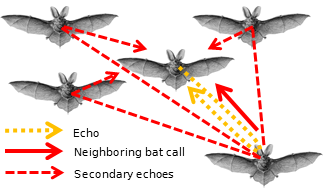
\includegraphics[]{original_papers/CPN_figures/Figure_1/cpn_sounds_schematic_012.png}
\centering
\caption{Schematic of the cocktail party nightmare. Arrows indicate the different types of sounds received by a focal bat: it needs to hear the echoes returning from its own calls (orange) to detect its neighbors, despite the masking by the calls of neighboring bats (solid red) and their secondary echoes (dashed red). Here, only 1 target echo off a single neighbor, only 1 representative neighboring bat call, and its set of secondary echoes are shown. In total, for a group of N bats, the focal bat will receive $N-1$ echoes, $N-1$ neighboring bat calls, and $N-1$x$N-2$ secondary echoes. Bat image courtesy of Wikimedia Commons/Ernst Haeckel.}
\label{cpn_fig1}
\end{figure}

\hypertarget{model-scenarios}{%
\subsection{Model Scenarios}\label{model-scenarios}}

We ran 2 model scenarios to test the effect of 1) increasing group size and of 2) variation in call parameters, group geometry, and acoustic parameters on neighbor detection. In all models, we used the central-most bat in the group as the focal bat.

\begin{itemize}
\tightlist
\item
  Scenario 1: \emph{Effect of group size on neighbor detection:} We simulated groups of 5,10, 30, 50, 75, 100, and 200 well-aligned bats with identical echolocation and hearing properties flying at a minimum inter-bat distance of 0.5 m (Table \ref{tab:modelscenarios} for full model parameters). The number and location of neighbors detected by the focal bat were recorded in every simulation run.
\item
  Scenario 2: \emph{Effect of call parameters, group geometry, and acoustic parameters on neighbor detection:} Here, we varied other parameters relevant to the cocktail party nightmare (Table \ref{tab:modelscenarios}) while keeping group size constant (\(N_{bats}\)=100, i.e.~the largest group size from Scenario 1 with a biologically relevant neighbordetection rate). We varied call parameters (interpulse interval, call duration,source level), group parameters (heading variation, minimum inter-bat spacing), and acoustic parameters (atmospheric absorption, acoustic shadowing).
\end{itemize}

\begin{table}

\caption{\label{tab:modelscenarios}Model parameters for both model scenarios: Scenario 1 modeled the effect of group size, while other parameters were fixed, resulting in 7 parameter combinations (1 per group size). Scenario 2 modeled the effect of other relevant parameters, while group size was kept constant at 100 bats, resulting in a combined set of 1,200 parameter combinations.}
\centering
\begin{tabular}[t]{>{\centering\arraybackslash}p{4cm}>{\centering\arraybackslash}p{4cm}>{\centering\arraybackslash}p{4cm}}
\toprule
Parameter & Scenario 1: Effect of group size & Scenario 2: Effect of call parameters, group geometry, and acoustics\\
\midrule
Group size & 5, 10, 30, 50, 75, 100, 200 & 100\\
Interpulse interval (ms) & 100 & 25, 50, 100, 200 ,300\\
Call duration (ms) & 2.5 & 1, 2.5\\
Source level (dB SPL re 20 $\mu$Pa at 1m) & 100 & 94, 100, 106, 112, 120\\
Minimum interneighbour distance (m) & 0.5 & 0.5,1.0\\
\addlinespace
Group heading variation ($^{\circ}$) & 10 & 10, 90\\
Atmospheric attenuation (dB/m) & -1 & 0, -1, -2\\
Acoustic shadowing & Yes & No, Yes\\
\bottomrule
\end{tabular}
\end{table}

\hypertarget{model-implementation}{%
\subsection{Model Implementation}\label{model-implementation}}

Each model run simulated 1 interpulse interval of the focal bat, and we calculated the timing and received level of all sounds (target echoes, masking calls, and secondary echoes) that arrived at the focal bat during that interpulse interval. Each model run simulated a series of sounds that arrived during an interpulse interval following the focal bats' call, based on a spatially explicit distribution of a group of bats (SI Appendix, Schematic \ref{cpn_schem_1}). At the beginning of every model run, \emph{N} bats were placed in a 2D space with randomly assigned heading directions (SI Appendix, \ref{cpn_groupgeom} and \ref{cpn_headingvar}). For each neighboring bat, we calculated its angle and distance to the focal bat. The received level was calculated based on a common source level for all bats, spherical and atmospheric spreading over each call's and echo's travel distance, and acoustic shadowing. Acoustic shadowing is the reduction in received level of a sound due to obstructions in its path. A sound in the cocktail party nightmare may pass around obstacles (other bats) as it propagates from source to receiver. The reduction in received level was measured and calculated as a linear function of the number of bats obstructing the path between source and receiver (SI Appendix \ref{cpn_shadowing}).For target and secondary echoes, we also considered monostatic and bistatic target strengths measured in this paper (SI Appendix, \ref{cpn_targetstrength}).

The arrival time of target echoes within the interpulse interval was determined according to the 2-way travel time to the echo-reflecting neighboring bat. The arrival time of masking calls and secondary echoes was assigned randomly with uniform probability across the interpulse interval. The random arrival time assignment of calls and secondary echoes recreates the uncoordinated echolocation of all bats in the group. It is unlikely that multiple bats in large groups can coordinate their calls effectively, and independent calling has been reported even in small groups of 4 bats (\citet{hase2018a}).

All bats in a group were identical in their calling properties, and we treated all sounds as constant tones of equal duration, i.e., we did not explicitly model spectral emission, propagation, and reception properties. The only difference between each of the sounds was their path and source of sound production. The omission of spectral properties is a conservative choice that assumes maximal masking of the primary echoes, thus allowing us to study the role of intensity differences and temporal separation between target echoes and masking sounds.

Once we calculated the timing and received level of all sounds at the focal bat, we accounted for directional hearing sensitivity (SI Appendix, Figure \ref{cpn_figS3}) and spatial unmasking. Spatial unmasking describes the reduction in experienced masking as the arrival angle between masker and target sound increases (\citet{ebata2003a}, \citet{suemer2009a}). We simulated spatial unmasking by the reduction of a masker's effective received level based on its angular separation to an echo. For each echo, the same masker will have a different effective masking level as its relative angle of arrival will be unique for each echo. We thus calculated the effective masking level of each masker for each echo. The effective masking levels of all maskers were then combined to form a time-variant and echo-specific ``masker SPL profile'' (SI Appendix, Figure \ref{cpn_figS5}D). This is essentially the joint sound pressure level (SPL) of all maskers over time. We then expressed this echo-specific masker SPL profile in relation to the echo's SPL, thus obtaining a relative ``echo-to-masker ratio profile'' (SI Appendix,Figure \ref{cpn_figS5}E). This is equivalent to a signal-to-noise ratio profile, where the echo is the signal and the masker profile is the noise.

In addition to angular separation, signal detection is also determined by the temporal separation between signal (echo) and masker (\citet{m1989a},\citet{yost2007a},\citet{siewert2004a}). Masking increases as the masker arrives closer in time to the echo. Masking occurs over longer durations when maskers arrive before the signal (forward masking) than afterward (backward masking). We recreated the asymmetric masking by a ``temporal masking envelope'' temporally centered at the echo (SI Appendix, Figure \ref{cpn_figS1}). The echo was considered heard if the echo-to-masker ratio profile was above the temporal masking envelope. We allowed short drops of the echo-to-masker ratio profile below the temporal masking envelope, for a combined maximum duration of less than 25\% of an echo's duration. Alternatively, we defined an echo to be masked (= not heard), if the echo-to-masker ratio profile was below the temporal masking envelope for more than 25\% of the echo duration. The 25\% threshold was an arbitrarily chosen conservative value to prevent masking by rare and short bursts of high sound pressure level that are unlikely to affect echo detection biologically (SI Appendix, \ref{cpn_detneighbour}).

\hypertarget{model-parametrization}{%
\subsection{Model Parametrization}\label{model-parametrization}}

We implemented a detailed set of echolocation, group and sound properties in our model, including call and hearing directionality, spatial unmasking, temporal masking, group geometry, and details of sound propagation. These properties were parameterized based on published results wherever available. Acoustic shadowing and target strengths (monostatic and bistatic) of bats were specifically measured for this work. All details of the model parameters including our respective measurements and on model implementation are presented in the Supporting Information.

\hypertarget{results}{%
\section{Results}\label{results}}

\hypertarget{effect-of-group-size-on-neighbor-detection}{%
\subsection{Effect of Group Size on Neighbor Detection}\label{effect-of-group-size-on-neighbor-detection}}

At group sizes of 5 and 10, the focal bat hears the echoes of most or all of its neighbors per call (median: 4 and 8 echoes per call at \emph{N}=5 and 10, respectively; Figure \ref{cpn_fig2}). At progressively larger group sizes, the median number of detected neighbors drops from 4 to 0 at group sizes of 30 to 200. Yet even in a group of 100 bats, while the median number of detected neighbors is zero, the 90th percentile is 1, showing that a neighbor is not detected with each call, but occasionally. Beyond a group of 100 bats, the focal bat typically detects no neighbors at all. The initial rise in detected neighbors in groups of 5 to 30 bats is primarily caused by the increased number of neighbors that could be detected, which is soon counter-acted by the intense masking that rises non linearly with group size.

We next derived the probability of detecting at least 1 neighbor per call, which describes the average rate of neighbor detection (Figure \ref{cpn_fig3}A, blue). At smaller groups of 5 to 30 bats, the focal bat detects at least 1 neighbor per call at above 0.95 probability. At larger group sizes (50 to 100), the probability of detecting at least 1 neighbor drops rapidly to 0.3 per call in a group of 100 bats, and is basically zero for a group of 200 bats (0.004 probability). A bat (with 10 Hz calling rate) flying in a group of 100 bats will thus detect at least 1 neighbor around 3 times per second (\textasciitilde 3 Hz detection rate), while a bat flying in a group of 30 bats will detect at least 1 neighbor almost every time it calls (9.5 Hz detection rate). The probability of detecting multiple bats per call is lower than just detecting at least 1 bat (Figure \ref{cpn_fig3}A). Yet,even in a group of 50 bats, the focal bat has a probability of detecting at least 2 and 4 neighbors per call of about 0.5 and 0.1, respectively.

We next quantified which neighbors the focal bat detects. Detection is generally limited to nearby neighbors (Figure \ref{cpn_fig3}B) and, with increasing group size, to neighbors in front of the focal bat (Figure \ref{cpn_fig3}C). At a group size of 30 bats, the focal bat occasionally detects neighbors that are up to 2 m away in radial distance, which is the furthest neighbor distance. With increasing group sizes, despite the group being more spread out, the focal bat can only detect its nearest neighbors (e.g., neighbors at \textasciitilde0.5 m in a group of 200 bats; Figure \ref{cpn_fig3}B). In the azimuthal plane, at small group sizes, the focal bat initially detects neighbors all around it (95\%-neighbor detection angle range≥237° for up to 50 bats; Figure \ref{cpn_fig3}C). With increasing group size, a frontal bias in neighbor detection appears (95\%-neighbor detection angle range: 191 to 35° for 100 and 200 bats; Figure \ref{cpn_fig3}C).

\begin{figure}[!htbp]
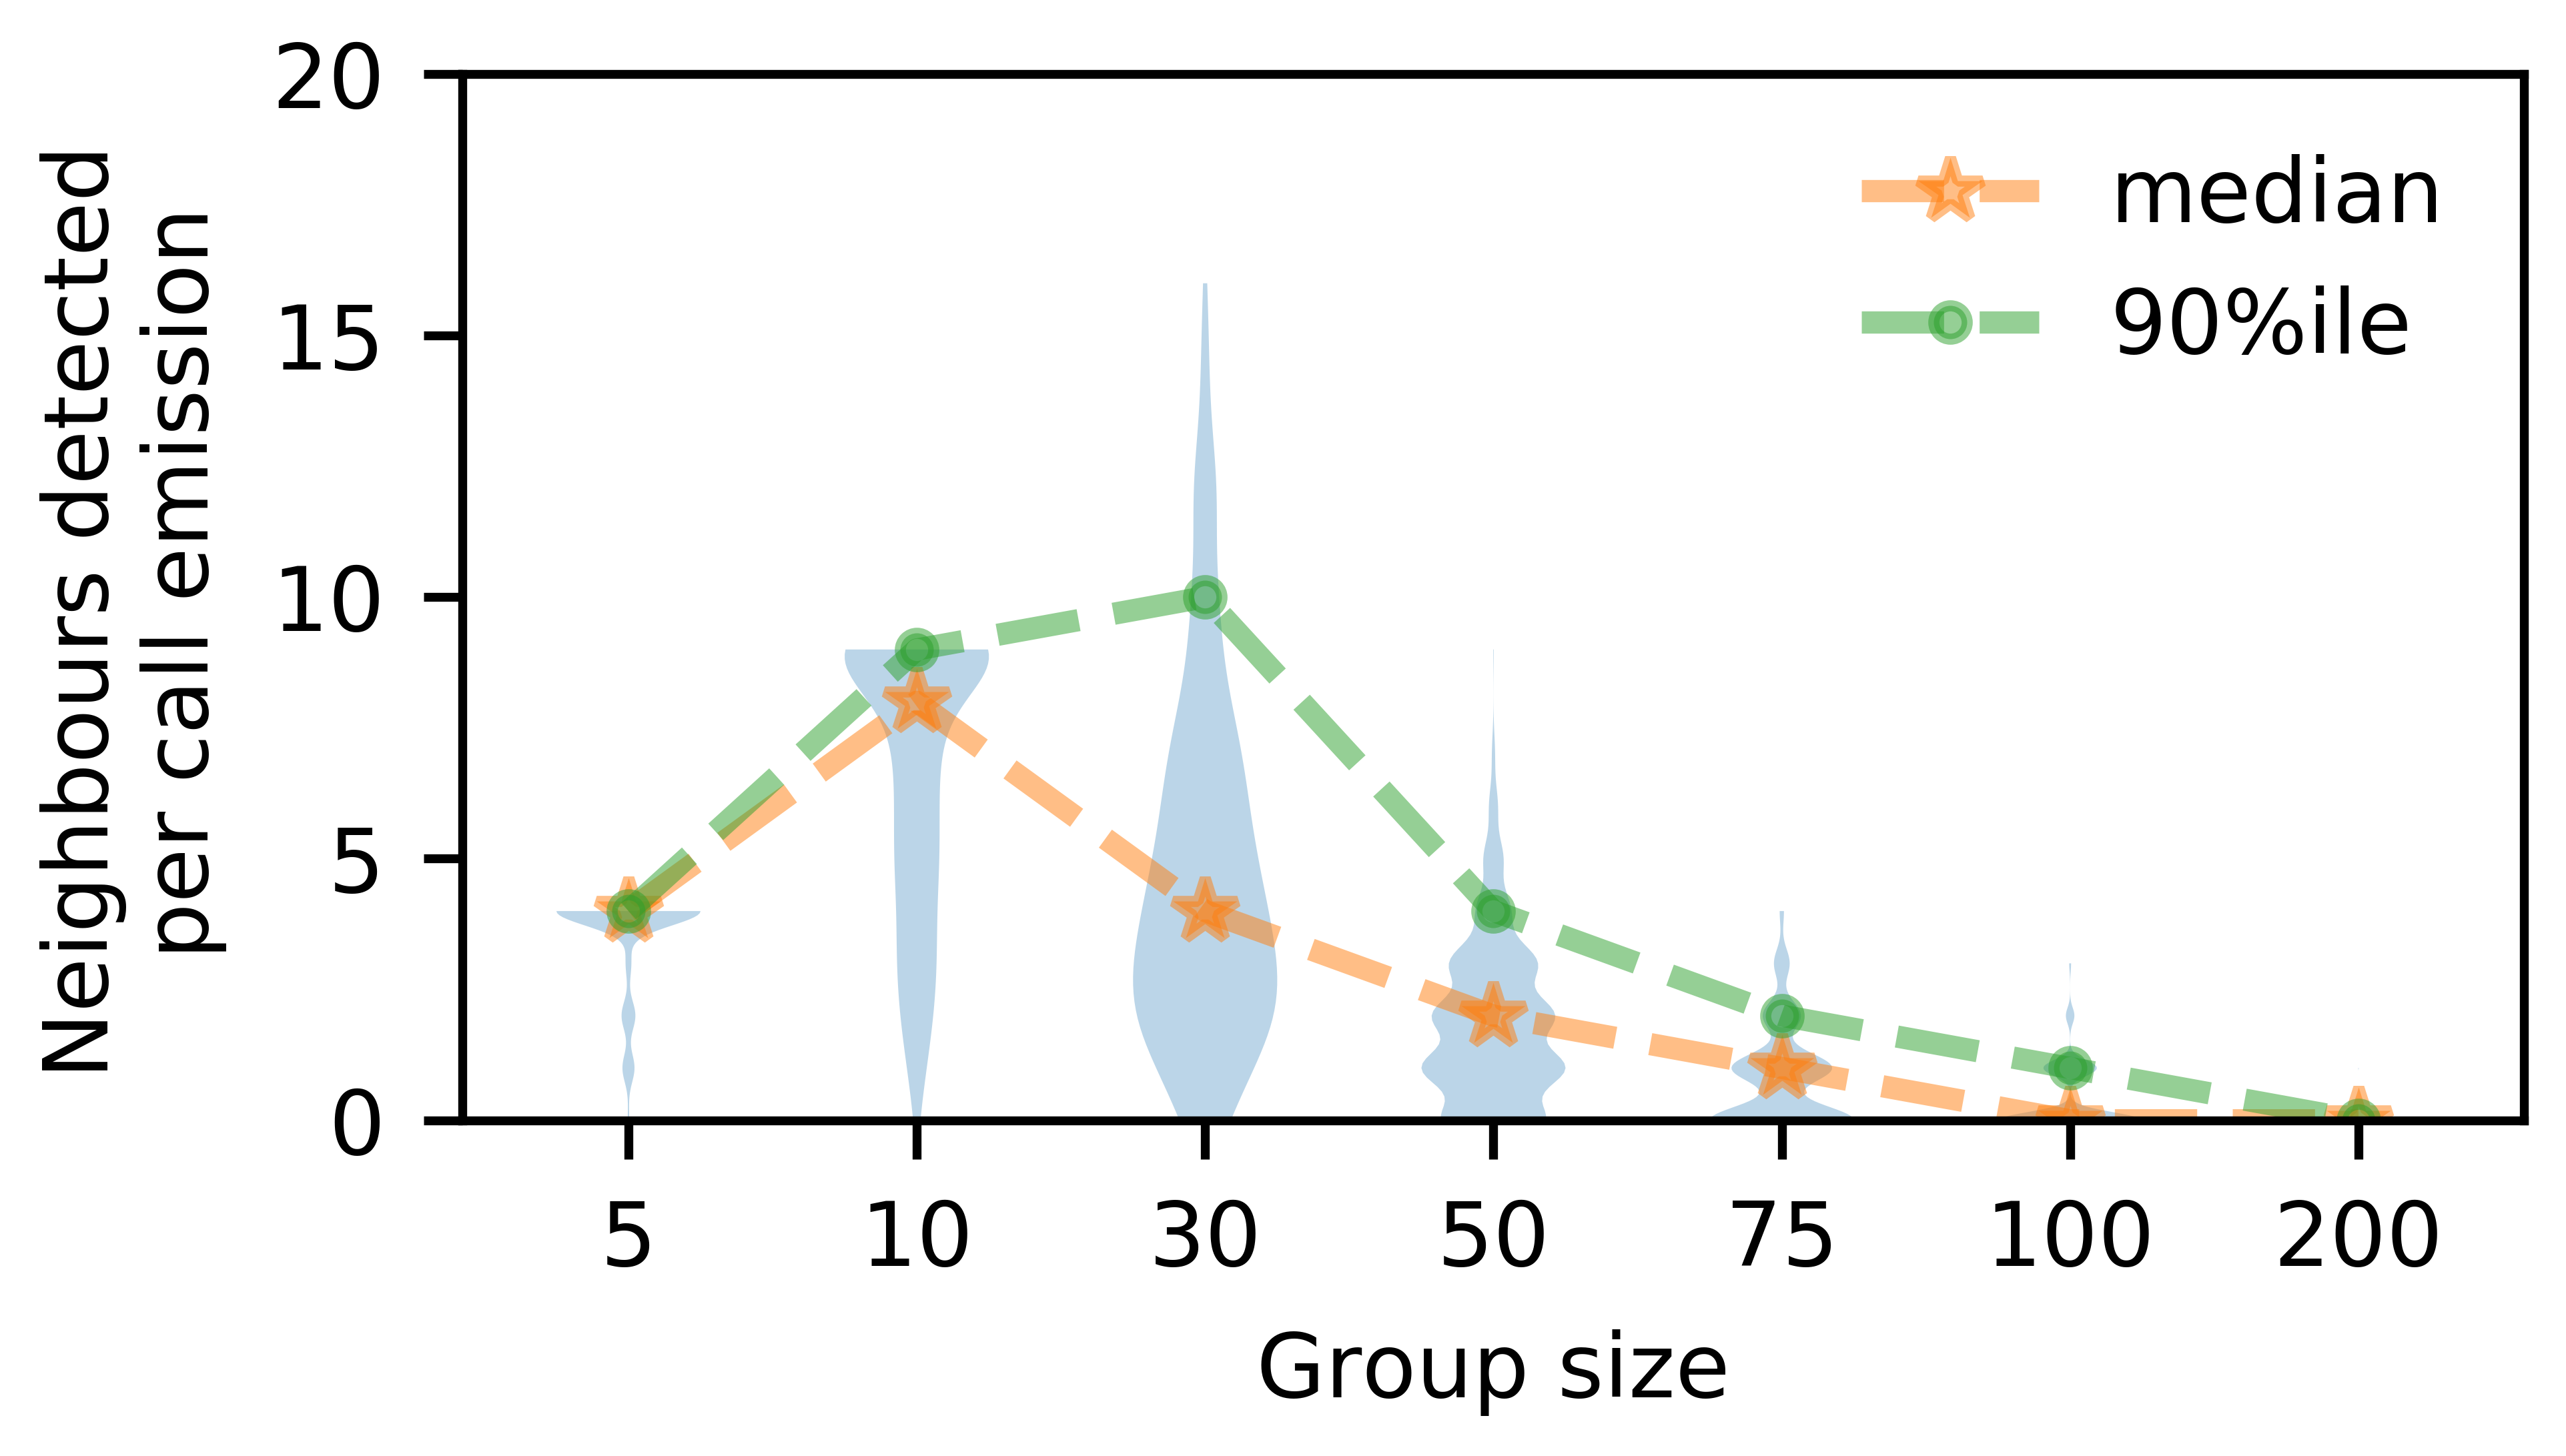
\includegraphics[]{original_papers/CPN_figures/Figure_2/Figure2_groupsize_1200dpi.png}
\centering
\caption{Number of detected neighbors per call by a focal bat in the center of a group. The initial rise in the number of detected neighbors is because there are indeed more neighbors and the degree of masking is low. However, with increasing group size, most of the neighbors cannot be detected anymore, and progressively fewer neighbors are detected per call. Violin plots show the distribution of the number of neighbors detected per call, and their median (stars, orange) and 90th percentile (dots, green).}
\label{cpn_fig2}
\end{figure}

\begin{figure}[!htbp]
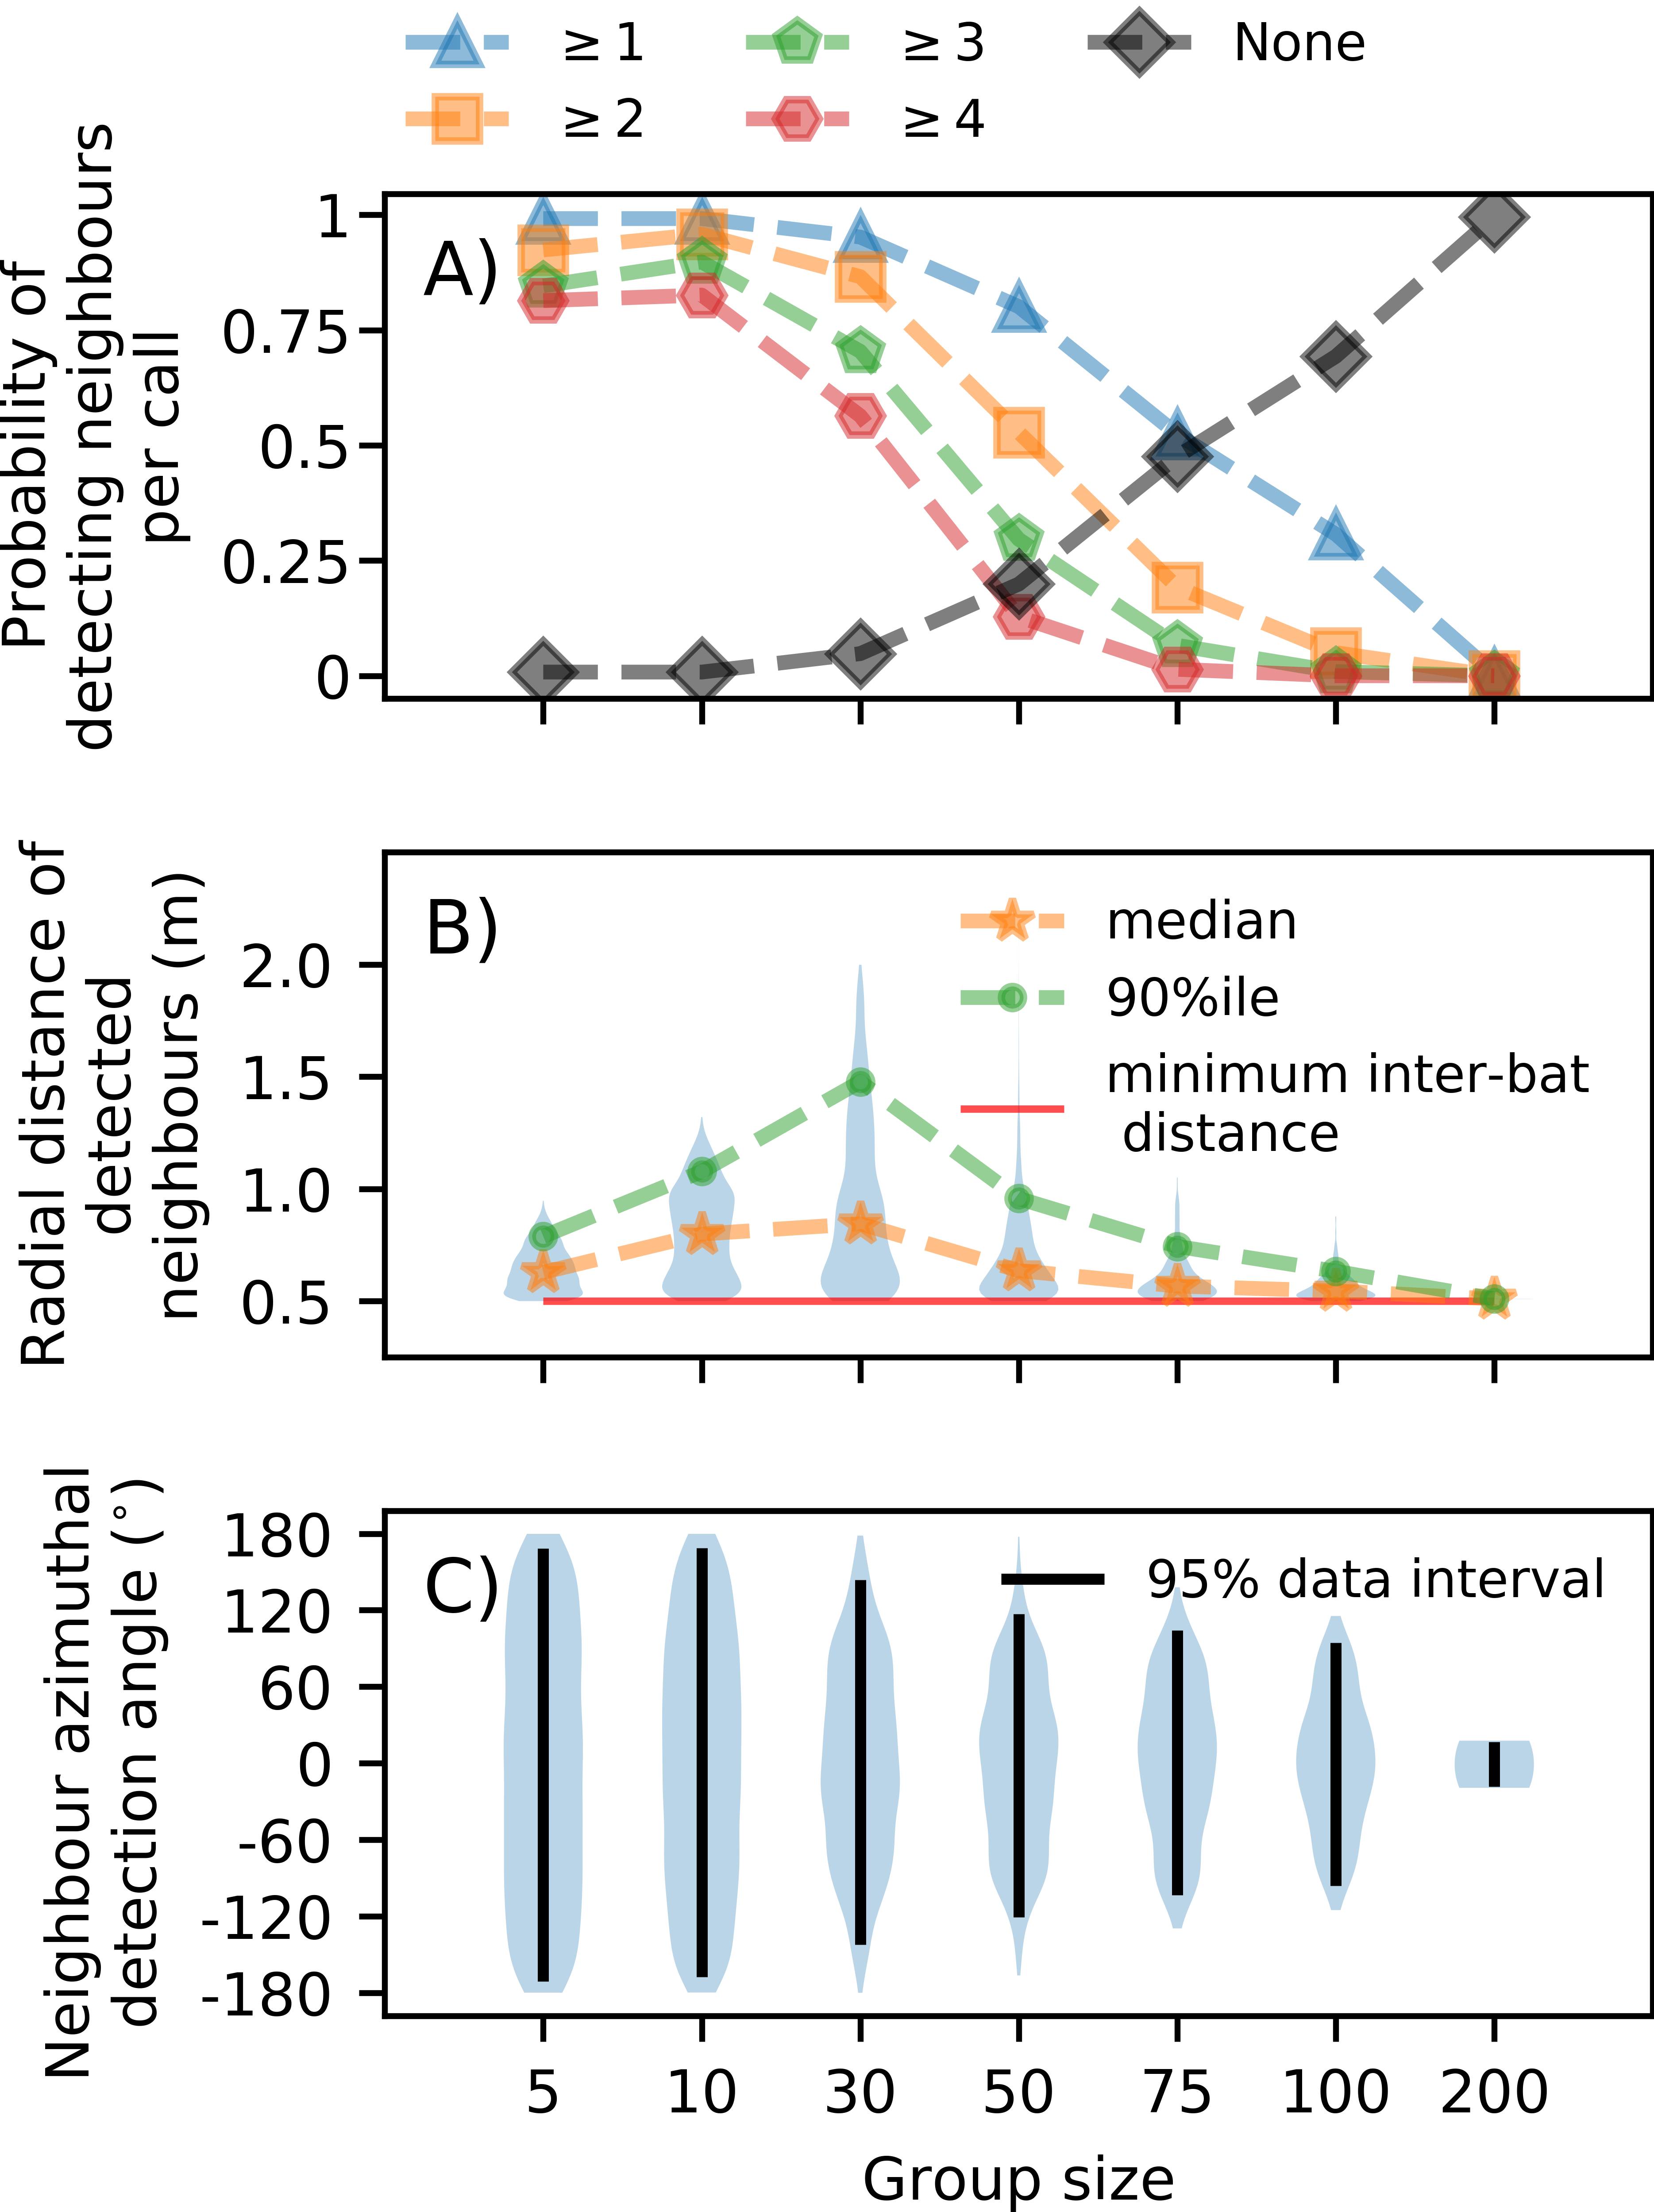
\includegraphics[]{original_papers/CPN_figures/Figure_3/Figure3_1200dpi_tight.png}
\centering
\caption{Characterization of the focal bat’s perception. (A) The probability of detecting $\leq X$ neighbors per call ($X$ = 1,2,3,4, or none). Even in groups of up to 100 bats, the focal bat has a \textasciitilde0.3 probability of detecting at least 1 neighbor
per call. In even larger groups (200 bats), no neighbors are detected anymore. (B) With increasing group size, a focal bat only detects its closest neighbors. Initially, the radial distance of detected neighbors increases because the spatial extent of a group increases with group size (at 5, 10, 30 bats: radius = 0.75, 1.12, 1.97 m), but it then drops down to the nearest neighbors beyond 30 bats. (C) The azimuthal location of detected neighbors, showing an increasing frontal bias with increasing group size. Although neighbors were uniformly distributed in azimuth, the frontal bias of call and hearing directionality means that frontal returning echoes are louder than peripheral ones.} 
\label{cpn_fig3}
\end{figure}

\hypertarget{effect-of-call-parameters-group-geometry-and-acoustic-parameters-on-neighbor-detection}{%
\subsection{Effect of Call Parameters, Group Geometry, and Acoustic Parameters on Neighbor Detection}\label{effect-of-call-parameters-group-geometry-and-acoustic-parameters-on-neighbor-detection}}

We next analyzed how variation in call parameters, group structure, and acoustic parameters affected neighbor detection. We fixed the group size to 100, as at this size,the focal bat could typically detect at most 1 neighbor (90\%ile, Figure \ref{cpn_fig2}) at 0.3 probability (Figure \ref{cpn_fig3}A) per call. We thus reduced the output of each simulation run to a binary neighbor detection score of 1 (detection) or 0 (no detection). We analyzed the effect of each parameter on neighbor detection with a logistic regression, treating all parameters as categorical and using their value in Scenario 1 as reference (parameter range in Table \ref{tab:modelscenarios}).

The call parameters interpulse interval and call duration showed the strongest effect (Figure \ref{cpn_fig4}A,B and SI Appendix, Table \ref{cpn_table2}). Increasing the interpulse interval from 100 ms to 200 and 300 ms increases neighbor detection probability by about 15 and 75 times, while reducing it to 50ms lowers neighbor detection to 0.05 times Scenario 1 (Figure \ref{cpn_fig4}A).Shortening call duration from 2.5 ms to 1 ms led to 35 times higher neighbor detection (Figure \ref{cpn_fig4}B). Call source level had no effect (Figure \ref{cpn_fig4}C).

Group geometry also influenced neighbor detection probability,but less than changing call parameters. Flying at larger interbat distances of 1.0 m leads to 0.31 times lower neighbor detection compared to denser groups with 0.5 m interbat distance (Figure \ref{cpn_fig4}D). Groups where individuals head in a more variable direction have 1.32 times better neighbor detection than groups with a generally common heading (or echolocation beam) direction (Figure \ref{cpn_fig4}E).

Among the physical parameters, acoustic shadowing increased neighbor detection (without acoustic shadowing, neighbor detection is 0.75 times lower than with acoustic shadowing), while atmospheric attenuation had a negligible effect (Figure \ref{cpn_fig4}F and G)

\begin{figure}[!htbp]
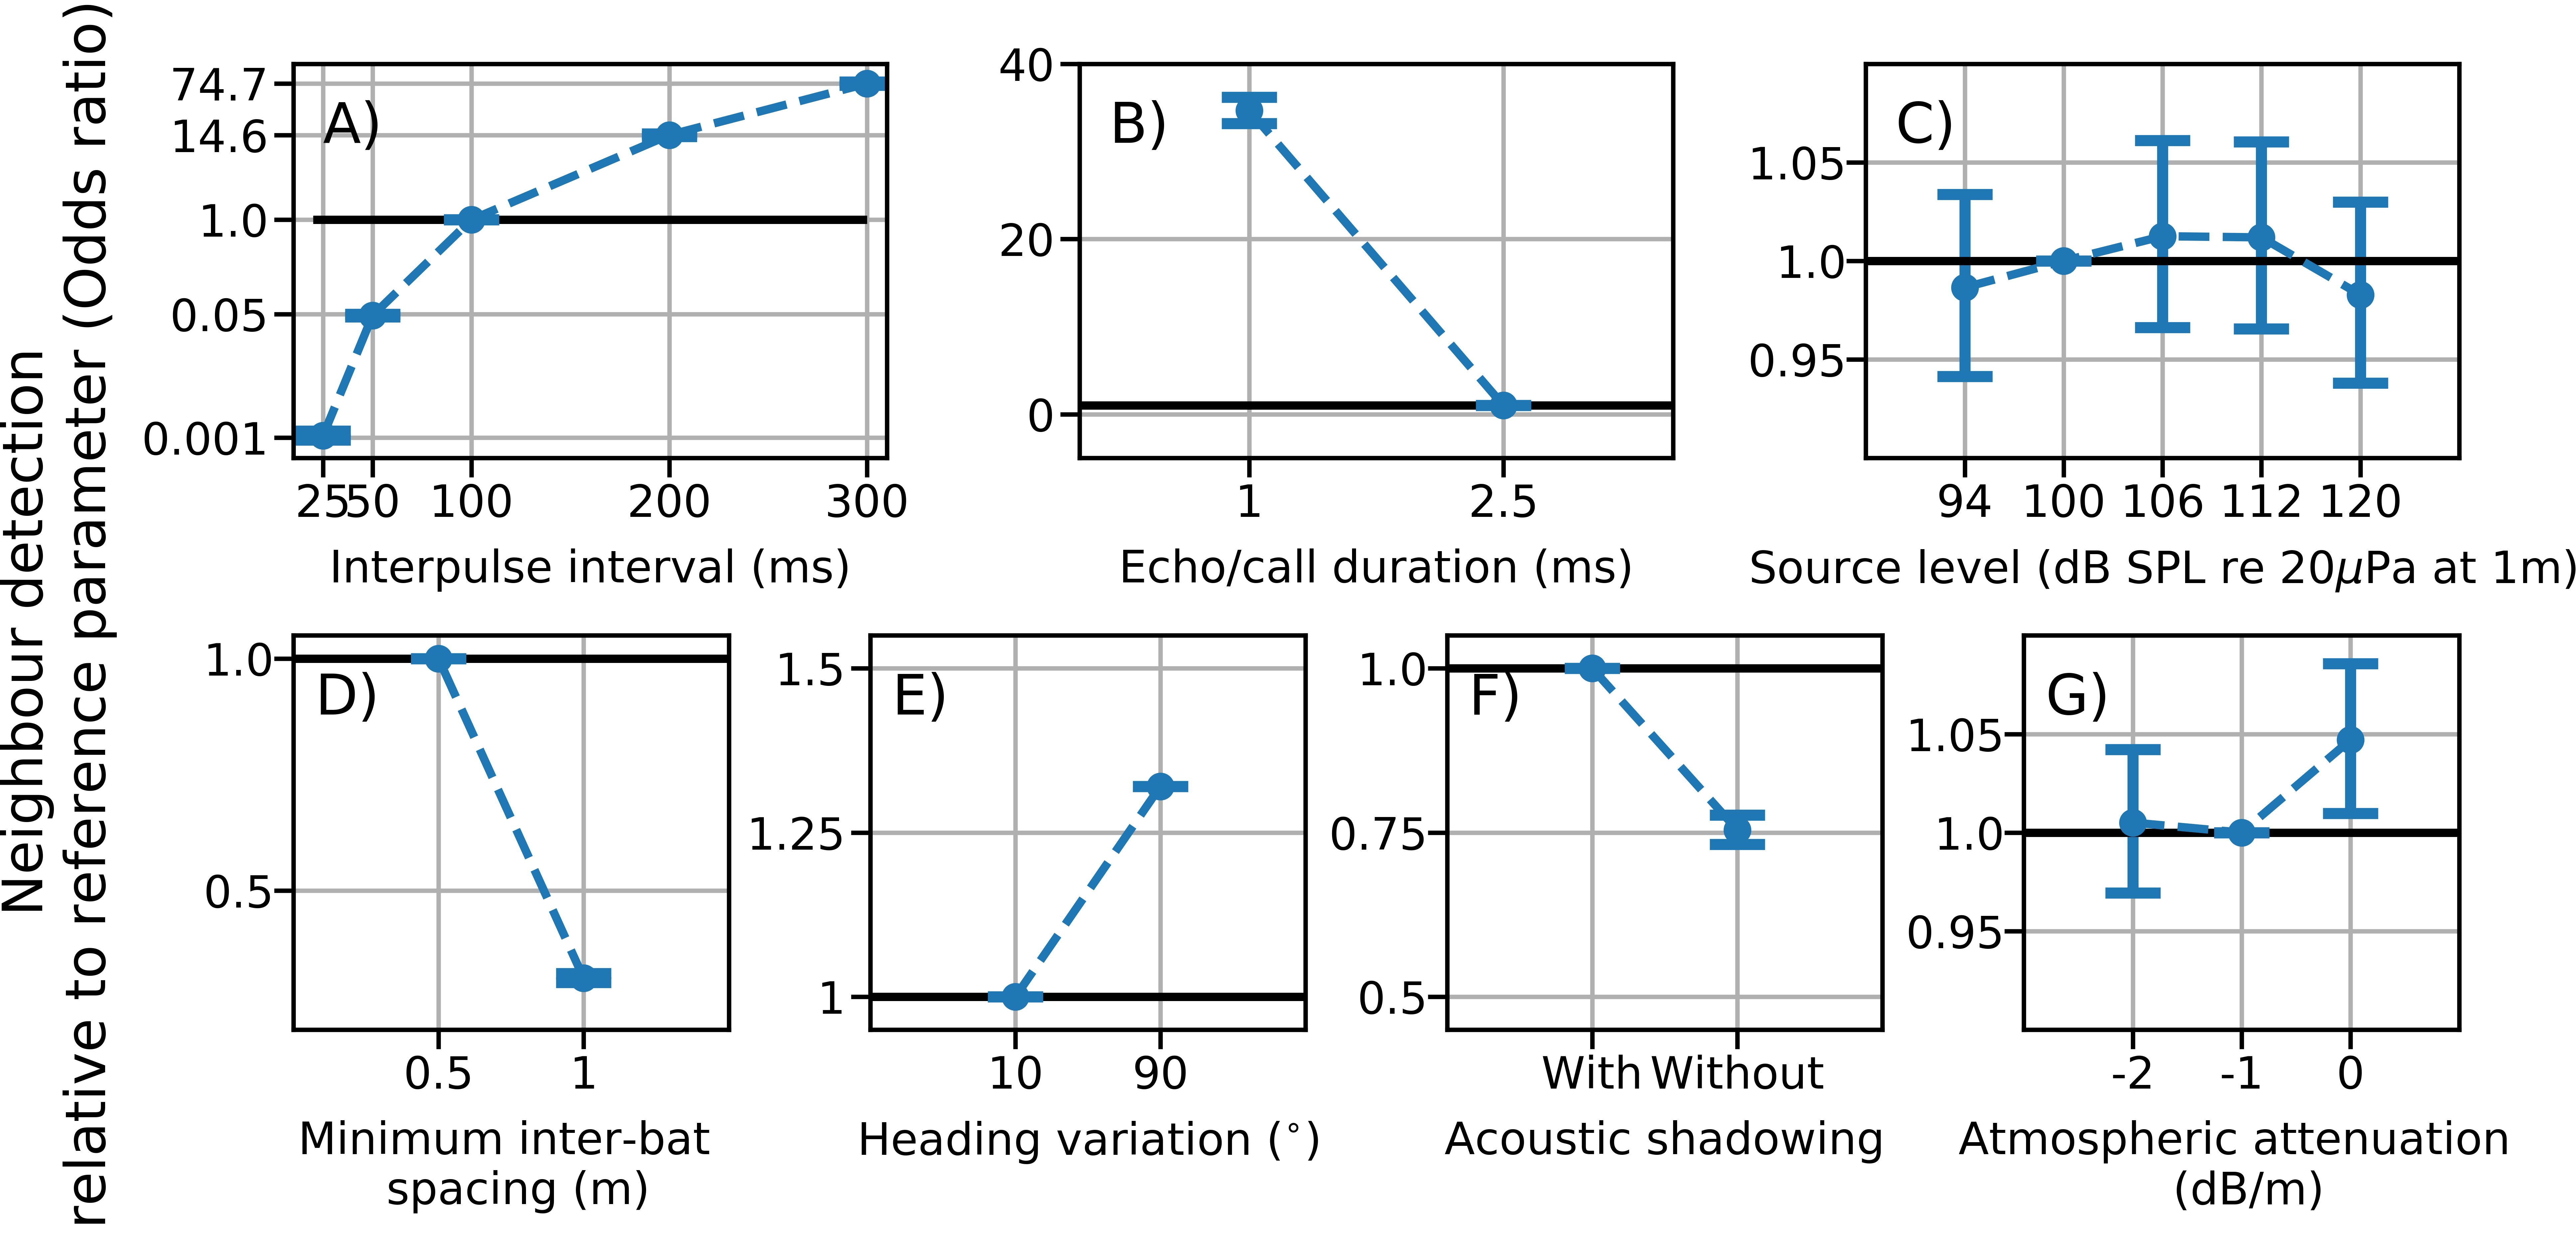
\includegraphics[]{original_papers/CPN_figures/Figure_4/Figure4_oddsratio_comparison.png}
\centering
\caption{Effect of call parameters (A–C), group geometry (D and E), and acoustic parameters (F and G) on neighbor detection. Each plot shows the probability of neighbor detection (model estimate and 95$\%$ confidence interval of odds ratio) when changing model parameters relative to the reference parameter used in the simulations of Scenario 1 (Table \\ref{tab:modelscenarios}). Odds ratios above and below 1 indicate a higher and lower neighbor detection probability, respectively, indicated by the horizontal reference line. (A–C) Call parameters: Longer interpulse intervals (A) and shorter call durations (B) increase neighbor detection probability, while call source level (C) has no effect. (D and E) Group geometry: Neighbor detection is better in groups that are tightly packed (D) and with higher heading variation (E). (F and G) Effect of acoustic parameters: Acoustic shadowing by bats in groups improves neighbor detection probability (F), while atmospheric attenuation has a negligible effect (G)} 
\label{cpn_fig4}
\end{figure}

\hypertarget{discussion}{%
\section{Discussion}\label{discussion}}

We present a conceptual framework to quantify what a focal bat experiences in the sonar cocktail party nightmare. We quantified the probability of detecting neighbors across a range of group sizes, which allows calculating the rate at which a focal bat detects its neighbors. When flying alone, a focal bat will detect objects around it at a rate equal to its call rate, while in a group,its object detection rate is reduced due to masking. We show that even in a group of 100 bats, bats still detect at least 1 neighbor per call about 3 times per second (for a 10 Hz call rate), while in smaller group sizes, neighbor detection rate is larger at 5 to 10 Hz. Bat echolocation is generally ``stroboscopic,''meaning that information is received intermittently with time gaps (\citet{griffin1958a}). We suggest that bats in smaller group sizes still experience a sufficiently high information update rate for performing collision avoidance and neighbor following. With increasing group size, perception might become ``hyper-stroboscopic,''i.e., so scarce that different sensorimotor heuristics might be required to maintain group coordination.

The low level of masking at smaller group sizes allows the focal bat to detect all its neighbors per call. With increasing group size, however, the focal bat detects maximally 1 neighbor per call in a group of 100 bats. This neighbor detection rate of at least 1 neighbor per call even in large group sizes provides a formal sensory basis for group movement in active sensing animals. While a bat in a large group cannot track the position of all its neighbors, it still can track the movement of a few neighbors, specifically those close to and in front of it. This reduction in rate, range, and direction of detected neighbors has predictive consequences for the kind of collective behavior bat groups may show in nature. Many models of collective movement assume that each individual in a group detects the position and orientation of neighbors in the whole of its sensory volume, and then performs an averaging across all neighbors to decide its next movement (\citet{couzin2002a},\citet{g2004a},\citet{t1995a},\citet{reynolds1987a}), leading to the impressive coordinated behaviors of fish schools and insect swarms (\citet{sumpter2006a},\citet{vicsek2012a}). As the number of neighbors that an individual detects decreases, more ``limited interactions'' begin to dominate, causing anisotropy in the group structure (\citet{bode2011a},\citet{ballerini2008a}). For bats in the cocktail party nightmare, we predict that large groups may show higher anisotropy than smaller groups due to the limited number of neighbors that they can detect and react to. All things being equal, we predict that in large groups (\textgreater50 bats), the neighbors in the frontal field of a bat will have a disproportionate influence on its movement decisions. Bats in larger groups may thus maintain higher alignment with their frontal neighbors compared to bats in smaller groups.

Our simulations allow for a direct quantitative comparison of the effects of echolocation, group geometry, and acoustic parameters in group echolocation. Among the call parameters tested, reducing call rate (increasing interpulse interval) was most effective in increasing neighbor detection in jamming conditions, matching experimental evidence for reduced calling rate in \emph{Tadarida brasiliensis} (\citet{jarvis2013a}, \citet{adams2017a}). In contrast, other FM bat species increase their call rates in groups and background noise(\citet{amichai2015a},\citet{lin2016a},\citet{cvikel2015b},\citet{luo2015a}). Likewise, our result that shorter call duration should improve neighbor detection is opposite to experiments showing that most bat species increased call duration in the presence of maskers (11, 23, 24, 43, 44), except (\citet{cvikel2015b}). Lastly, our result of no effect of changing source level on neighbor detection might also seem to differ from experimental data showing that bats in laboratory conditions do increase source level in the presence of maskers (\citet{amichai2015a},\citet{tressler2009a},\citet{luo2015a},\citet{hase2016a}). While there might be species-specific variation, we suggest that these differences are mostly due to the experimental situation. Bats in these experiments experienced constant maskers. Calling more often, for longer, and louder thus improved the bats' signal redundancy, echo-to-masker ratio, and overall echo detection. In contrast, our model simulates group flight of many bats with simultaneous and uniform changes in their call parameters. When all bats in a group shorten call duration, this reduces the overall duration of masking sounds, thus improving echo detection. Likewise, when all bats in a group increase their call amplitudes to optimize their own echo-to-masker ratios, all bats will eventually call at their maximum, with no overall effect on neighbor detection. Analyzing bat calls in mass emergences is technically challenging and it remains unknown whether \emph{T. brasiliensis} and other gregarious bat species reduce their call rate in the field.

Bat aggregations show a variety of structures across behavioral contexts, from well-aligned almost parallel flight during roost emergences, to more variable and less-aligned flight in mating swarms and when circling in limited cave volumes. We show that this group structure itself affects how well bats can detect each other. Bats detect their neighbors better in less-aligned groups compared to more aligned groups. During aligned emergence flight, the focal bat always receives loud forward-directed masking calls from bats behind it, in addition to the relatively loud side-calls emitted by neighbors to its left and right. In contrast, during less-aligned swarming flight, the relative orientation of the bats is more distributed and changing, with the focal bat experiencing a wider dynamic range of masker levels (i.e., louder and fainter masking calls originating from a wider range of angular directions). This increased dynamic masker range allows for better echo detection, as there will be drops in echo-to-masker ratios due to changing received masker level. This effect is beneficial for enabling swarming flight, as the collision risk in less-aligned flight is likely higher compared to the more aligned emergence flights. Inter-individual distance is another parameter of group structure,and we show that neighbor detection is better in dense groups. This might seem unexpected given that the received SPL of the maskers is higher the closer the bats are to each other. However, received echo levels are also higher when bats are closely spaced. Since echo SPL drops by 12 dB per doubling of distance, but masker call SPL only by 6 dB per doubling of distance, the echo-to-masker ratio is higher at shorter compared to longer inter-bat distances. It would be interesting to examine if perhaps large groups in the field actually fly closer to each other than smaller groups.

While we only modeled neighbor detection for the central-most bat in a group, its position in the group (e.g., central, frontal, or at the back) is likely to also have an effect on the number and received level of maskers, and thus on the number of detected echoes. However, we expect the obtained trends to remain qualitatively the same regardless of focal bat position. Particularly, we predict that masking will increase with group size, and only the exact group size at which a given level of masking (e.g., X\% neighbor detection probability) is obtained will change depending on the focal bat's position in the group.

We furthermore show that it is important to consider bats not only as sources of reflected echoes and masking sounds, but also as obstructions to sound that actually alleviate the cocktail party nightmare. Typically, the detected echoes originate from nearby bats and are not shadowed. In contrast, the masking calls and secondary echoes can arrive from distant neighbors, thus passing by multiple other bats. Shadowing thus consists of the overall reduction in masker levels, which increases echo-to-masker ratios for the comparatively loud echoes returning from nearby neighbors.

Our results show that the cocktail party may not be as much of a ``nightmare'' as previously thought (\citet{ulanovsky2008a}). We show that the modeled psychoacoustic, spatial, and acoustic properties act together to alleviate the nightmare into a challenge. When bats are flying in a multi echo environment, our results show that a bat will always hear some echoes after a call emission, and very rarely no echoes at all. This parallels the phenomenon of auditory ``glimpsing'' reported in the human auditory cocktail party where individuals may follow conversations by perceiving parts of detected speech rather than whole sounds (\citet{miller1950a}).

\hypertarget{improved-echo-detection-in-real-world-situations}{%
\subsection{Improved Echo Detection in Real-World Situations}\label{improved-echo-detection-in-real-world-situations}}

We present a first approximation to the sonar cocktail party nightmare, including many relevant biological, physical, and auditory mechanisms. Bats are expert echolocators and can detect echoes and fly under challenging conditions (\citet{m1989a}, \citet{surlykke1992a},\citet{petrites2009a},\citet{bates2008a}). Bats rapidly adjust their call behavior in terms of their call duration, source level, and interpulse intervals (\citet{luo2017a}, \citet{corcoran2017a}), integrate echoic information over multiple call emissions (\citet{simmons2012a}), and actively track objects by aiming their calls at them (\citet{ghose2006a}, \citet{ghose2006b}). While we tested a range of differentecholocation call parameters, our model implemented these parameters as fixed values that do not vary over time, thus lacking the dynamic nature of a real bat in the wild.

Furthermore, we did not model the spectral content of echo ormasker sounds, and analyzed echo detection based on a fixedthreshold of echo-to-masker-ratio. In contrast, real echolocation calls possess a time-variant spectral pattern that is species and even individual specific (\citet{gillam2010a}, \citet{yovel-a}), which can reduce echo masking. Masking is strongest when target and masker overlap both intime and in frequency (i.e., fall within the same critical band ofthe auditory system) (\citet{ebata2003a}, \citet{fletcher1940a}). The frequency-modulation of bat calls means that even when maskers and echoes partially overlap in time, they will not necessarily overlap in frequency, thus reducing the likelihood of masking. The individuality of bat calls may help a bat reject the secondary echoes from other bats' calls by forming separate auditory streams (\citet{fay2008a}) for its own echoes and others' echoes. Given the scarcity of empirical data to parametrize the effect of spectral differences on echo detection in masking conditions, we did not include it in our model, thus simulating a conservative worst case scenario where all sounds lie in the same frequency band. Additionally, attentional processes strongly improve target detection by improving the signal-to-noise ratio in the presence of maskers with similar time-frequency structure (\citet{hafter2008a}). Under real-world conditions, it is likely that masking in groups is even less than simulated here.

Due to the scarcity of published data, the inter-individual and interspecific variation in the temporal and spatial masking functions used in our model is unknown. The temporal masking envelope will arguably be similar in many bat species, showing the typical mammalian pattern of worse target detection threshold with shorter temporal separation between target and masker. Spatial unmasking occurs through the nonlinear interaction of pinnae shape, cochlear and higher auditory processing (\citet{ebata2003a}, \citet{culling-a}). As pinna shape and associated acoustic receiver characteristics strongly vary in echolocating bats (\citet{obrist1993a}), this will lead to species-specific spatial unmasking and echo detection rates in the sonar cocktail party nightmare.

\hypertarget{conclusion}{%
\section{Conclusion}\label{conclusion}}

We provide a conceptual framework to explain how active sensing animals such as echolocating bats successfully navigate in groups despite mutually jamming each other. The intense jamming in groups might lead to individuals only detecting their nearest frontal neighbors, which might drive limited interactions within a group. We also show that call parameters and group geometry determine the challenge in the sonar cocktail party nightmare. Recent advances in on-body acoustic tags (\citet{cvikel2015b}, \citet{stidsholt2018a}), signal analysis(\citet{aodha2018a}), and acoustic tracking (\citet{seibert2015a}) of echolocating animals in the field might facilitate future experimental validation of our model predictions. As our model formulation is not constrained to echolocation in bats, it can be parametrized to other echolocators such as oilbirds, swiftlets, and odontocetes (\citet{brinkl2013a}, \citet{surlykke2014a}) that also echolocate in groups and suffer from cocktail-party--like conditions.

\hypertarget{acknowledgements}{%
\subsection{Acknowledgements}\label{acknowledgements}}

We thank the members of the Acoustic and Functional Ecology Group for insightful comments and support, Claire Guérin for contributing to code development, the Max Planck Institute for Ornithology for excellent research infrastructure, and 2 anonymous reviewers for helpful comments. T.B. was funded by a doctoral fellowship from the German Academic Exchange Service (DAAD) and the International Max Planck Research School for Organismal Biology. H.R.G. was funded by the Emmy Noether program of the German Research Foundation (DFG, GO 2091/2-1, GO 2091/2-2).The simulation runs in this paper were funded by a Google (Research Credits) grant to T.B.

\newpage

\hypertarget{supplementary-information}{%
\section{Supplementary Information}\label{supplementary-information}}

\newpage

\hypertarget{model-parametrization-1}{%
\subsection{Model parametrization}\label{model-parametrization-1}}

Here, we present the details of how we parametrized our model of the sonar cocktail party nightmare, based on empirical data of behavioral studies in bats and our own measurements.

\hypertarget{temporal-masking-envelope}{%
\subsubsection{\texorpdfstring{Temporal masking envelope \label{cpn_tempmasking}}{Temporal masking envelope }}\label{temporal-masking-envelope}}

We derived the echo-to-masker sound pressure level (SPL) ratios for forward, backward and simultaneous masking from two empirical target-detection studies in echolocating bats (Table \ref{tab:maskingtable}). We only chose studies where the target and masker were co-located along the same direction. Both studies presented the ratio between the echo and masker SPL at target detection for various delays between
echo and masker arrival time. We linearly interpolated (in a piecewise fashion) the echo-to-masker SPL ratios between each of the time delays measured in the studies to obtain the full temporal masking envelope ranging from -0.65 and +24 ms delay of the target echo relative to the masker edge (Figure \ref{cpn_figS1}).

\hypertarget{spatial-unmasking-function}{%
\subsubsection{\texorpdfstring{Spatial unmasking function \label{cpn_spatiunmasking}}{Spatial unmasking function }}\label{spatial-unmasking-function}}

Sümer et al.~(2009) performed a backward masking study to address spatial unmasking in the bat \emph{Eptesicus fuscus}. In a two-alternative forced-choice paradigm, they increased the angular separation between a target object and a masker object while also varying the level of the target object's echo (by varying the size of the target object and thus its target strength).

We define the spatial unmasking function as the echo-to-masker SPL ratio at just-noticeable echo detection as a function of angular separation. To obtain the echo-to-masker level ratios, we subtracted the target object's target strengths from the masker object's target strength. We normalized the spatial unmasking function to the co-localised echo-masker case (i.e., when both echo and masker arrive from the same direction). This describes the reduction in echo-to-masker ratio required for echo detection as a function of angular separation between target and masker,compared to the co-localized case. We digitized the data points from Figure \ref{cpn_fig4}B of Sümer et al.~(2009) by hand with WebPlotDigitiser \citep{rohatgi2015a} to obtain the target's target strength as a function of angular separation. Masker target strength was given by Sümer et al.~(2009) as -14.5 dB. We then calculated the target-masker SPL ratios and interpolated them with a quadratic polynomial fit (Figure \ref{cpn_figS2}). The interpolated data was then further upsampled to 0.47° intervals. As Sümer et al.~(2009) only measured angular separations up to 23°. We conservatively used the echo-masker SPL ratio at 23° also for all larger angular separations.

\hypertarget{call-and-hearing-directionality}{%
\subsubsection{\texorpdfstring{Call and hearing directionality \label{cpn_directionality}}{Call and hearing directionality }}\label{call-and-hearing-directionality}}

Echolocation calls have a directional beam shape, meaning that the emitted SPL
generally decreases with increasing angular distance from the main call direction, which has the highest call SPL (Figure \ref{cpn_figS3}). The highest call SPL is typically towards the front, and reduces towards the back of the bat. Despite this directionality and additional variation with call frequency and behavioral context \citep[\citet{l2013a},\citet{surlykke2012a},\citet{giuggioli2015a}]{jakobsen2010a} , bats still emit a significant amount of sound pressure into the backward direction. The average call SPL behind a bat is about 14 dB lower than in the forward direction \citep[\citet{stidsholt2018a}]{giuggioli2015a}. Call directionality leads to a drop in the effective number of masking calls from neighbors as only those calls arriving from a limited range of directions will have sufficiently high SPL (Figure \ref{cpn_figS3}). For example, in an emergence situation with approximately parallel flight directions, the focal bat will receive the loudest calls from those bats flying behind it. Similarly, the lowest received call levels in an emergence will be from those bats flying in front of the focal bats.

Like call production, hearing is also directional. The pinna structure of a bat
attenuates or amplifies the same sound depending on its direction of arrival \citep[\citet{f2008a}]{firzlaff2003a}. In \emph{Myotis daubentonii}, hearing directionality between 35-45 kHz leads to an average amplification of frontally arriving sounds by 4 dB in comparison to those arriving from behind. We used data of Giuggioli et al (2015) to describe the average call and hearing directionality of our modelled bats (Figure \ref{cpn_figS3}).

\hypertarget{atmospheric-attenuation}{%
\subsubsection{\texorpdfstring{Atmospheric attenuation \label{cpn_atmabs}}{Atmospheric attenuation }}\label{atmospheric-attenuation}}

Ultrasound in air is heavily attenuated by atmospheric attenuation, even over short distances of a few meters \citep[\citet{lawrence1982a}]{h2018a}. Atmospheric attenuation will reduce the received SPL of a masker or echo at the focal bat. We chose a range of values for the atmospheric attenuation coefficient α between 0 to -2 dB/m. These values approximate the atmospheric attenuation experienced by a bat calling at very low (\(\leq\) 20 kHz, \textasciitilde0 dB/m) to high (60 kHz, \textasciitilde-2 dB/m) peak frequencies.

\hypertarget{geometric-attenuation}{%
\subsubsection{\texorpdfstring{Geometric attenuation \label{cpn_geomattn}}{Geometric attenuation }}\label{geometric-attenuation}}

Sound pressure level reduces with increasing distance from the source, called
geometric attenuation. For all sounds in our model (target echoes, masking calls
and secondary echoes), we implemented spherical geometric spreading, i.e.,
uniform spreading of sound in all directions \citep{speaks1996a}.

\hypertarget{group-geometry}{%
\subsubsection{\texorpdfstring{Group geometry \label{cpn_groupgeom}}{Group geometry }}\label{group-geometry}}

A group of bats might organize themselves tightly or well spread in the field. The spacing between bats will decide how loud the returning target echoes, masking calls and secondary echoes are. We simulated a group of bats by placing individual bats on a 2D plane using the Poisson disk algorithm \citep{bridson2007a}. The advantage of using the Poisson disk algorithm is that points are spaced relatively uniformly in space compared to a random placement of points from two independent distributions. The other advantage of the Poisson disk algorithm is that it allows the specification of a minimum distance between two points. For the first simulations varying group size only, we chose 0.5 m as inter-bat distance (see Table \ref{tab:modelscenarios}, main text), matching the average interbat-distance in dense swarms of T. brasiliensis in the field \citep{theriault2010a}. In addition to 0.5 m minimum inter-bat distance, we also studied how a sparser 1.0 m minimum inter-bat distance affects neighbor detection (see Table \ref{tab:modelscenarios}, main text). The Poisson disk arranged bats showed average inter-bat distances of between 1-1.5 times the specified minimum distance between points.

\hypertarget{heading-variation}{%
\subsubsection{\texorpdfstring{Heading variation \label{cpn_headingvar}}{Heading variation }}\label{heading-variation}}

Active sensing animals are known to `scan' their environments by emitting energy
in varying directions of interest according to the behavioral context \citep[\citet{bullock2005a}]{wisniewska2015a}. Bats alter the shape and direction of their sonar beam while they fly \citep[\citet{ghose2006a}, \citet{w2017a}]{jakobsen2010a}. The directions into which each bat in a group aims its calls could affect how well each bat in the group can detect echoes. A group of bats calling into the same direction may experience high masking, as a focal individual will receive many loud calls from the bats behind it. In contrast, a group of bats calling into a larger range of directions may experience less masking. The focal bat may receive a mix of fainter off-axis calls and loud on-axis calls from neighbors.

We simulated the scanning behavior of individual bats in the group by setting a
heading angle for each individual. Each individual called into the direction of its heading angle, and we chose two levels of variation of heading angles in the group. Groups with a low heading variation were all pointing their beams in more or less the same direction. Groups with high heading variation were pointing their beams in a wider range of directions. A low heading variation simulates an emergence situation where each bat is calling approximately into the overall flight direction of the group. A high heading variation simulates a swarming situation where each bat is calling at a unique direction. Given the lack of empirical data to guide our estimates, we chose \(\pm\) 10° for the low heading variation, and \(\pm\) 90° for the high heading variation. The heading angle for each individual was randomly drawn from a uniform distribution covering the respective range.

\hypertarget{monostatic-and-bistatic-target-strength-of-a-flying-bat}{%
\subsubsection{\texorpdfstring{Monostatic and bistatic target strength of a flying bat \label{cpn_targetstrength}}{Monostatic and bistatic target strength of a flying bat }}\label{monostatic-and-bistatic-target-strength-of-a-flying-bat}}

Quantifying the received levels of echoes and secondary echoes requires
knowledge of the target strength of a bat when emitter and receiver are at the same and at different locations. Here, we measured monostatic and bistatic target strengths \citep{richards2010a} of a flying stuffed \emph{Myotis myotis} bat. Monostatic target strengths refer to the situation where the emitter and receiver are at the same location, i.e.,they are the same bat (this is the `classical' target strength usually considered in echolocation research). Bistatic target strength refers to a situation where the emitter and receiver are at different locations, i.e., the receiving bat hears the echo of a call that was emitted by another bat, i.e.~a secondary echo.

In the simulations, all incoming and outgoing sounds at the bat are between abs(0-180)°. Sounds with 0° angle are along the heading direction of the focal bat. Sounds arriving/reflecting on the left have negative angles (0° \(\geq \theta \geq\)-180°), and those on the right have positive angles (0° \textgreater{} \(\theta\) \textgreater180°).

\textbf{Methods}: We ensonified a stuffed \emph{Myotis myotis} with outstretched wings, which was suspended from the ceiling at \textasciitilde1 m height and placed on a rotating base, which could be rotated in 45° steps. A speaker (electrostatic Polaroid, custom built) and microphone (CM16/CMPA, Avisoft Bioacoustics, Glienicke, Germany) were placed at a 1 m radial distance to the center of the bat (Figure \ref{cpn_figS4}). The speaker emitted linear frequency modulated sweeps between 96-20 kHz, with durations of 170 \(\mu\)s, 1 ms and 2 ms at 92 dB rms SPL re 20 μPa at 1 m. The speaker was driven by a custom-built amplifier with input from a soundcard (Player 216H, Avisoft Bioacoustics, 1 MHz sampling rate). The microphone signal was recorded simultaneously with an attenuated version of the speaker signal on a multichannel soundcard (USG 416H, Avisoft Bioacoustics, 500 kHz sampling rate). The microphone had a noise floor of 24 dB rms SPL re 20 μPa. All echoes were recorded at \(\geq\) 22dB signal-to-noise ratio. The experiment was performed in the middle of a large empty room (\textasciitilde4x4x2 m) to temporally separate bat echoes from background echoes.

We ensonified the bat from front (0°) to back (180°) in steps of 45°. We assumed
that the bat was symmetrical and thus did not ensonify angles from 180-360°. The
angular separation between the speaker and the microphone was also altered in
steps of 45° between -180° to +180°. This resulted in 40 target strength
measurements (5 sound directions x 8 angular separations).

The integrated target strength \citep{j1985a} of the recordings were calculated by subtracting the energy of recordings with the bat from those without the bat at the expected time window of echo arrival. The echo level was calculated in rms by taking the square root of the energy.

\textbf{Results}: The monostatic target strength of a flying stuffed \emph{Myotis myotis} bat at various orientations was between -43 and -34 dB at 1 m distance, matching the general range of previously published values \citep{goetze2016a}. The bistatic target strength, which was used to calculate the received level of the secondary echoes, was between -44 and -10 dB across all combinations of emitter-receiver locations. For further details on experimental protocol, raw data and reproduction of generated results, please refer to the archived Jupyter notebooks at this link: \url{https://doi.org/10.5281/zenodo.3469845} .

\hypertarget{acoustic-shadowing-in-bat-groups-with-varying-number-of-bats-and-inter-bat-spacing}{%
\subsubsection{\texorpdfstring{Acoustic shadowing in bat groups with varying number of bats and inter-bat spacing \label{cpn_shadowing}}{Acoustic shadowing in bat groups with varying number of bats and inter-bat spacing }}\label{acoustic-shadowing-in-bat-groups-with-varying-number-of-bats-and-inter-bat-spacing}}

As multiple bats fly together in a group, the bats themselves will block all sounds travelling between an emitter and a receiver. Essentially, the bats themselves act as obstacles that cause acoustic shadowing, reducing the received sound pressure level at the focal bat. In a large group, multiple bats may shadow a sound as it moves from the emitter and to the receiver. We quantified acoustic shadowing in a series of playback experiments that varied the inter-bat spacing (0.5 and 1.0 m) and the number of bats (1 -- 6) in a line.

\textbf{Methods:} A microphone (CM16/CMPA, Avisoft Bioacoustics) and speaker
(Polaroid, custom-built) were placed at a fixed distance of 9.9 m apart, facing each other. We hung 1 to 6 ``model bats'' made of foam with paper wings at 0.5 or 1.0 m distance to each other from a string running above the speaker to the microphone. The designed model bat showed acoustic shadowing similar to that of the stuffed \emph{Myotis myotis} used in the target strength measurements described in \ref{cpn_targetstrength}.

The speaker was placed as far as possible from the microphone to calculate
acoustic shadowing without the effects of speaker directionality. The speaker
played back a variety of 7 ms Tukey windowed signals consisting of pure tones
(20, 35, 50, 100 kHz) and a downward modulated linear sweep (100-15 kHz). Each
signal type was played back 15 times at \textasciitilde4\% duty cycle. Multiple signal types were used to obtain a generalized estimate of shadowing across a wide range of call peak frequencies and call types. The playback signals and recordings are available here: \url{https://doi.org/10.5281/zenodo.3469845}. Additionally, we also recorded the same playback without model bats being present. We calculated acoustic shadowing as the reduction in received level by subtracting the received level (in dB rms) without bats from the received level with bats. We performed a linear regression of attenuation as a function of factors number of bats and inter-bat-distance, to estimate the amount of acoustic shadowing caused per bat and the spacing between them.

\textbf{Results}: Bats effectively shadowed the sound, with strong effects of the inter-bat-spacing and the number of bats. Bats at 0.5 m distance in front of the receiving bat (=microphone) reduced the received SPL by 5.17 dB (SEM=0.44, t=-11.639, 95\% CI =-6.05,-4.30), while bats at 1.0 m interbat-spacing reduced the received SPL by 1.85 dB (SEM=0.44, t=-4.164, 95\% CI =-2.72,-0.98). Each bat reduced received SPL by 0.83 dB (SEM=0.08, t=-9.852, 95\% CI =-0.99,-0.66).
For further details on experimental protocol, raw data and reproduction of
generated results, please refer to the archived Jupyter notebooks at this link:
\url{https://doi.org/10.5281/zenodo.3469845}.

\hypertarget{model-implementation-1}{%
\subsection{Model implementation}\label{model-implementation-1}}

Here, we present how we implemented the parameters described before into our
final model, and how our model was initialized and run.

\hypertarget{model-idea}{%
\subsubsection{Model idea}\label{model-idea}}

The idea of our model is to analyze the relative timing and sound pressure level
of target echoes, masking calls and secondary echoes at a focal bat flying in a
group of other bats. Each model iteration thus analyzed one single interpulse
interval, i.e., the time after emission of one call until the emission of the next call by the focal bat. Within that interpulse interval, the focal bat received the echoes from its own call that reflected off the neighboring bats, the calls of those neighboring bats, and the secondary echoes which originate from the calls of the neighboring bats reflecting off other neighboring bats (Figure \ref{cpn_fig1}, main text).

We placed groups of bats in a 2D plane with various inter-bat distances and
heading directions. We then calculated received timing and SPL of all sounds
based on realistic assumptions about call properties, mammalian auditory
characteristics and sound physics.

All echoes, calls and secondary echoes were considered to be equal in duration,
amplitude envelope, and frequency composition. Frequency composition was not
explicitly specified, which is a conservative modelling choice that maximizes
masking potential \citep{yost2007a} and makes our model generalizable to multiple bat species. All sounds were treated as having a constant amplitude envelope (i.e., no amplitude modulations), but they differed in the sound pressure level received by the focal bat.

\hypertarget{model-initialization}{%
\subsubsection{Model initialization}\label{model-initialization}}

Each model iteration consisted of distributing bats in a 2D plane and assigning
each bat a heading direction. This spatial distribution was used to calculate the arrival times and received level of target echoes, masker calls and secondary echoes within the interpulse interval (Figure \ref{cpn_fig1}). The interpulse interval was discretized into time bins of 1 \(\mu\)s duration. Each received target echo corresponded to one neighbor. The arrival time of each echo was calculated using twice the distance between focal and neighboring bat.

The arrival time of masker calls and secondary echoes were chosen randomly.
The random arrival time assignment of masker calls and secondary echoes is
supported by the finding that groups of \emph{Miniopterus fuliginosus} \citep{hase2018a} do not coordinate their calling behavior, and seem to echolocate independently.
Moreover, at large group sizes beyond a few bats it is unlikely that bats could effectively co-ordinate their call emission times.

\hypertarget{target-echo-properties}{%
\subsubsection{Target echo properties}\label{target-echo-properties}}

Target echoes are the echoes that the focal bat receives in response to its own
echolocation call. In our model, the target echoes are echoes reflected off the
neighboring bats. When a focal bat hears a target echo it means it has detected
the corresponding neighboring bat.

An echo was defined as a sound occupying a block of time within the interpulse
interval (Figure \ref{cpn_figS5}A). Echoes were simulated to arrive at delays corresponding to
the distance to the neighboring bat they reflected off, e.g.~if a neighboring bat was at 1 m distance to the focal bat, then its echo arrived at a delay of 6.06 ms (at 330 m/s sound propagation).

The received level of the returning echo was calculated based on emitted call
source level into the direction of the neighboring bat, our monostatic target strength
measurements of a bat, and geometric attenuation over the sound travel distance.
If acoustic shadowing and atmospheric absorption were included in a simulation
run, the received level was reduced based on the number of bats in the path and
the atmospheric attenuation for the overall distance travelled by the echo. Echo
arrival direction was determined based on the position of each neighboring bat.

\hypertarget{masker-call-properties}{%
\subsubsection{Masker call properties}\label{masker-call-properties}}

Masker calls arrived at random time points with uniform probability within the
interpulse interval (Figure \ref{cpn_figS5}B), based on the observed lack of call synchronization in groups of \emph{Miniopterus fuliginosus} \citep{hase2018a}. Call directionality was based on the directionality function in Giuggioli et al., 2015, who fit a cosine based function to describe the overall call directionality of \emph{Myotis daubentonii} echolocating in the field. We set the asymmetry parameter A to 7.0. We calculated the angle of call emission towards the focal bat for each conspecific bat based on its angular position (heading) and distance. We then calculated the effective source level into the direction of the focal bat by reducing the call's on-axis source level (Table \ref{tab:modelscenarios} in main text) according to the call directionality function and the focal bat's relative position to the conspecific (Figure \ref{cpn_figS3}). This reduced level was the final received level of the conspecific masker call. If acoustic shadowing and atmospheric attenuation were included in a simulation run, the received level was reduced based on the number of bats in the path and the overall distance travelled by the call.

\hypertarget{secondary-echo-properties}{%
\subsubsection{Secondary echo properties}\label{secondary-echo-properties}}

Like the masking calls, secondary echoes arrived randomly with uniform probability in the interpulse interval (Figure \ref{cpn_figS5}C). The received level of a secondary echo was based on the emitted call source level into the direction of the neighboring bat, our bistatic target strength measurements of a bat, and geometric attenuation over the sound travel distance. If acoustic shadowing and atmospheric absorption were included in a simulation run, the received level was reduced based on the number of bats in the path and the overall distance travelled by the secondary echo.

\hypertarget{obtaining-the-masker-sound-pressure-level-profile}{%
\subsubsection{Obtaining the masker sound pressure level profile}\label{obtaining-the-masker-sound-pressure-level-profile}}

All sounds were treated as having a fixed received level (no envelope
modulations). For each target echo, we calculated its unique masker SPL profile
based on the relative timing, relative arrival directions and received levels of all asking calls and secondary echoes. This masker SPL profile was different for
each target echo because the temporal and spatial properties of the masking
sounds differ for each echo, resulting in different received levels and spatial
unmasking (see main text for details). We first calculated the effective masker SPL for each masking sound by correcting for spatial unmasking based on the angular separation between the echo and the masker. All effective masker SPLs of all masking sounds together over time represent the complete masker sound
pressure profile for each target echo (Figure \ref{cpn_figS5}E). When two or more maskers
overlapped in time, we added their linear sound pressures to obtain their joint
masking SPL. This approach assumes that overlapping maskers are coherent
sound sources that constructively interfere. This is a conservative assumption that will maximize masking.

\hypertarget{determining-neighbor-detection-the-temporal-masking-envelope}{%
\subsubsection{\texorpdfstring{Determining neighbor detection: the temporal masking envelope \label{cpn_detneighbour}}{Determining neighbor detection: the temporal masking envelope }}\label{determining-neighbor-detection-the-temporal-masking-envelope}}

The masker SPL profile for each echo describes the received masking SPL over
time. From the masker SPL profile, we created an echo-to-masker ratio profile by
normalizing the SPL of the target echo to the masker SPL profile:

\emph{echo-to-masker ratio profile (dB) = echo level (dB SPL) -- masker sound pressure level (dB SPL)}

The echo-to-masker-ratio profile is comparable to a signal-to-noise-ratio: at 0 dB, echo and masker have the same SPL. The masker is louder than the echo for negative values, and the echo is louder than the masker for positive values.

To determine whether a given target echo was heard or not, we compared the echo-to-masker ratio for this echo with the temporal masking envelope (see \ref{cpn_tempmasking}). The temporal masking envelope describes the echo-to-masker ratio at which masking occurs as a function of relative timing between echo and masker. Using the temporal masking envelope is important because masking does not only occur when the masker coincides with the echo, but also when the masker does not overlap with the echo and arrives before (forward masking) or after (backward masking) it. In our case, echo and masker had durations of only 1-2.5 ms, while a masker arriving at up to \textasciitilde25 ms before and up to \textasciitilde1 ms after the echo still causes some amount of masking. Thus, our temporal masker envelope had a duration of either \textasciitilde27 or \textasciitilde28.5 ms (Figure \ref{cpn_figS5}F). We compared the echo-to-masker ratio profile to the temporal masking envelope. The echo was considered not heard if the echo-to-masker ratio profile lay below the temporal masking envelope, i.e., the echo-to-masker ratio was lower than required for echo detection. Alternatively, the echo was considered heard if the echo-to-masker ratio profile lay above the temporal masking function, i.e., the echo-to-masker SPL ratio was higher than required for echo detection.

However, as the echo-to-masker ratio continuously fluctuates over time, it is possible that it is not fully above or below the temporal masking envelope throughout the envelope's duration. We thus defined an echo to be masked (= not heard), if it was masked for more than 25\% of its duration (of 1 or 2.5 ms). To calculate the total duration of masking, we analyzed the total duration that the echo-to-masker ratio was below the temporal masking envelope. As long as the total masking duration was shorter than 25\% of the echo duration (of 1-2.5 ms) the echo was considered detected. If this duration was longer than 25\% of the echo duration, the echo was masked and the corresponding neighboring bat was considered not detected. This 25\% threshold was set to make the simulated
auditory system immune to short spikes in masking sound pressure level occurring during the temporal masking function.

\hypertarget{open-source-software-used-in-the-research}{%
\subsection{Open-source software used in the research}\label{open-source-software-used-in-the-research}}

All simulation code, experimental data and results were made possible through the use of the NumPy \citep{oliphant2006a}, SciPy \citep{virtanen2019a}, Pandas \citep{mckinney2010a}, Matplotlib \citep{hunter2007a}, Statsmodels \citep{seabold2010a}, sounddevice \citep{geier2015a}, Anaconda \citep{anaconda2016a} and CPython \citep{rossum1991a} open-source projects.

\hypertarget{acknowledgements-1}{%
\subsection{Acknowledgements}\label{acknowledgements-1}}

We thank Renate Heckel and Felix Hartl for contributing to and building the ensonification setup, Magnus Wahlberg for helpful discussions on the ensonifications, Henrik Brumm for permission to use Raum 1.03 for the ensonification experiments, and Mihai Valcu for facilitating simulation runs on the in-house server facility.

\newpage

\hypertarget{supplementary-schematics-tables-and-figures}{%
\subsection{Supplementary Schematics, Tables and Figures}\label{supplementary-schematics-tables-and-figures}}

\subsubsection{Echo detection pseudo-code}\label{cpn_schem_1}

Pseudo-code of the steps in a simulation run to determine the detected neighbors per call emission.

\begin{enumerate}
  \item Place \textit{N} bats in group with minimum inter-bat distance
  \item Choose bat closest to the center of the group as the focal bat
  \item Populate interpulse intervals with maskers and echoes:
    \begin{enumerate}
    \item Propagate maskers (calls and secondary echoes) and calculate their received levels according to the position and orientation of the source neighbors. Assign random timing within interpulse interval.
    \item Propagate echoes from focal bats' own call and calculate their arrival time and received levels according to the position and orientation of the neighbors.
    \end{enumerate}
  \item Implement hearing directionality of the focal bat: amplify the received level of all sounds according to their relative angle of arrival
  \item Per echo, determine if it was heard:
    \begin{enumerate}
      \item Implement spatial unmasking by reducing the effective received level of all masking sounds based on their angular separation to the echo
      \item Combine all maskers over time to form a 'masker profile'
      \item Calculate the 'echo-to-masker profile', with reference to the echo level
      \item Implement temporal masking by checking if the relative echo-masker profile lies below the temporal masking envelope centered on the echo's location in the interpulse interval.
    \end{enumerate}
\end{enumerate}

\newpage

\begin{table}

\caption{\label{tab:maskingtable}Target-detection studies in echolocating bats used to extract echo-masker SPL ratio for our model. The time delay is the time between the edge of a masker and the target echo. A positive time delay indicates forward masking (masker arrives before the target), a negative time delay indicates backward masking (masker arrives after the target).}
\centering
\begin{tabular}[t]{>{\centering\arraybackslash}p{2.5cm}>{\centering\arraybackslash}p{2.5cm}>{\centering\arraybackslash}p{2.5cm}>{\centering\arraybackslash}p{2.5cm}>{\centering\arraybackslash}p{2.5cm}}
\toprule
Publication & Species & Time delay (ms) & Masking condition & Echo-masker SPL (dB)\\
\midrule
Siewert et al. 2004 & \textit{Megaderma lyra} & 3 & Forward & -17\\
Siewert et al. 2004 & \textit{Megaderma lyra} & 6 & Forward & -23\\
Siewert et al. 2004 & \textit{Megaderma lyra} & 12 & Forward & -29\\
Siewert et al. 2004 & \textit{Megaderma lyra} & 24 & Forward & -34\\
Sümer et al. 2009 & \textit{Eptesicus fuscus} & -0.65 & Backward & -22.3\\
\bottomrule
\end{tabular}
\end{table}

\newpage

\begin{landscape}


\begin{table}

\caption{\label{tab:regressionresults}Results of the logistic regression to quantify the effect of different parameter values on the odds ratio to detect at least one neighbor. Odds ratio values >1 indicate a higher probability of neighbor detection, while odds ratios <1 indicate a lower probability of neighbor detection.}
\centering
\begin{tabular}[t]{c>{\centering\arraybackslash}p{1cm}>{\centering\arraybackslash}p{1cm}>{\centering\arraybackslash}p{1cm}>{\centering\arraybackslash}p{1cm}>{\centering\arraybackslash}p{1cm}>{\centering\arraybackslash}p{1cm}>{\centering\arraybackslash}p{1cm}>{\centering\arraybackslash}p{1cm}c}
\toprule
Parameter & Value tested & Reference value & Odds Ratio & Odds Ratio - 2.5 CI & Odds Ratio - 97.5 CI & Log Odds Ratio & Log Odds Ratio SEM & Z (log odds ratio estimate) & P >|z|\\
\midrule
Intercept &  &  & 0.32 & 0.31 & 0.35 & -1.11 & 0.027 & -40.51 & 0\\
Heading variation ($^{\circ}$) & $\pm$90 & $\pm$10 & 1.32 & 1.28 & 1.36 & 0.28 & 0.015 & 18.35 & 0.0\\
Acoustic shadowing & Yes & No & 0.75 & 0.73 & 0.78 & -0.28 & 0.015 & -18.63 & 0.0\\
Interpulse interval (ms) & 25 & 100 & 0.001 & 9e-04 & 0.001 & -6.84 & 0.073 & -93.52 & 0\\
 & 50 & 100 & 0.048 & 0.046 & 0.05 & -3.04 & 0.023 & -134.14 & 0\\
\addlinespace
 & 200 & 100 & 14.6 & 13.995 & 15.228 & 2.68 & 0.022 & 124.46 & 0\\
 & 300 & 100 & 74.68 & 70.497 & 79.122 & 4.31 & 0.029 & 146.49 & 0\\
Minimum interbat distance (m) & 1 & 0.5 & 0.31 & 0.301 & 0.321 & -1.17 & 0.016 & -72.83 & 0\\
Sound duration (ms) & 1 & 2.5 & 34.66 & 33.172 & 36.206 & 3.55 & 0.022 & 158.83 & 0\\
Source level (dB SPL re 20 $\mu$Pa at 1m) & 94 & 100 & 0.99 & 0.941 & 1.034 & -0.01 & 0.024 & -0.57 & 0.57\\
\addlinespace
 & 106 & 100 & 1.01 & 0.966 & 1.061 & 0.01 & 0.024 & 0.52 & 0.6\\
 & 112 & 100 & 1.01 & 0.966 & 1.061 & 0.01 & 0.024 & 0.5 & 0.62\\
 & 120 & 100 & 0.98 & 0.938 & 1.03 & -0.02 & 0.024 & 0.73 & 0.47\\
Atmospheric attenuation (dB/m) & 0 & -1 & 1.05 & 1.01 & 1.086 & 0.05 & 0.019 & 2.48 & 0.01\\
 & -2 & -1 & 1.01 & 0.97 & 1.042 & 0.01 & 0.018 & 0.27 & 0.78\\
\bottomrule
\end{tabular}
\end{table}

\end{landscape}

\newpage

\begin{figure}
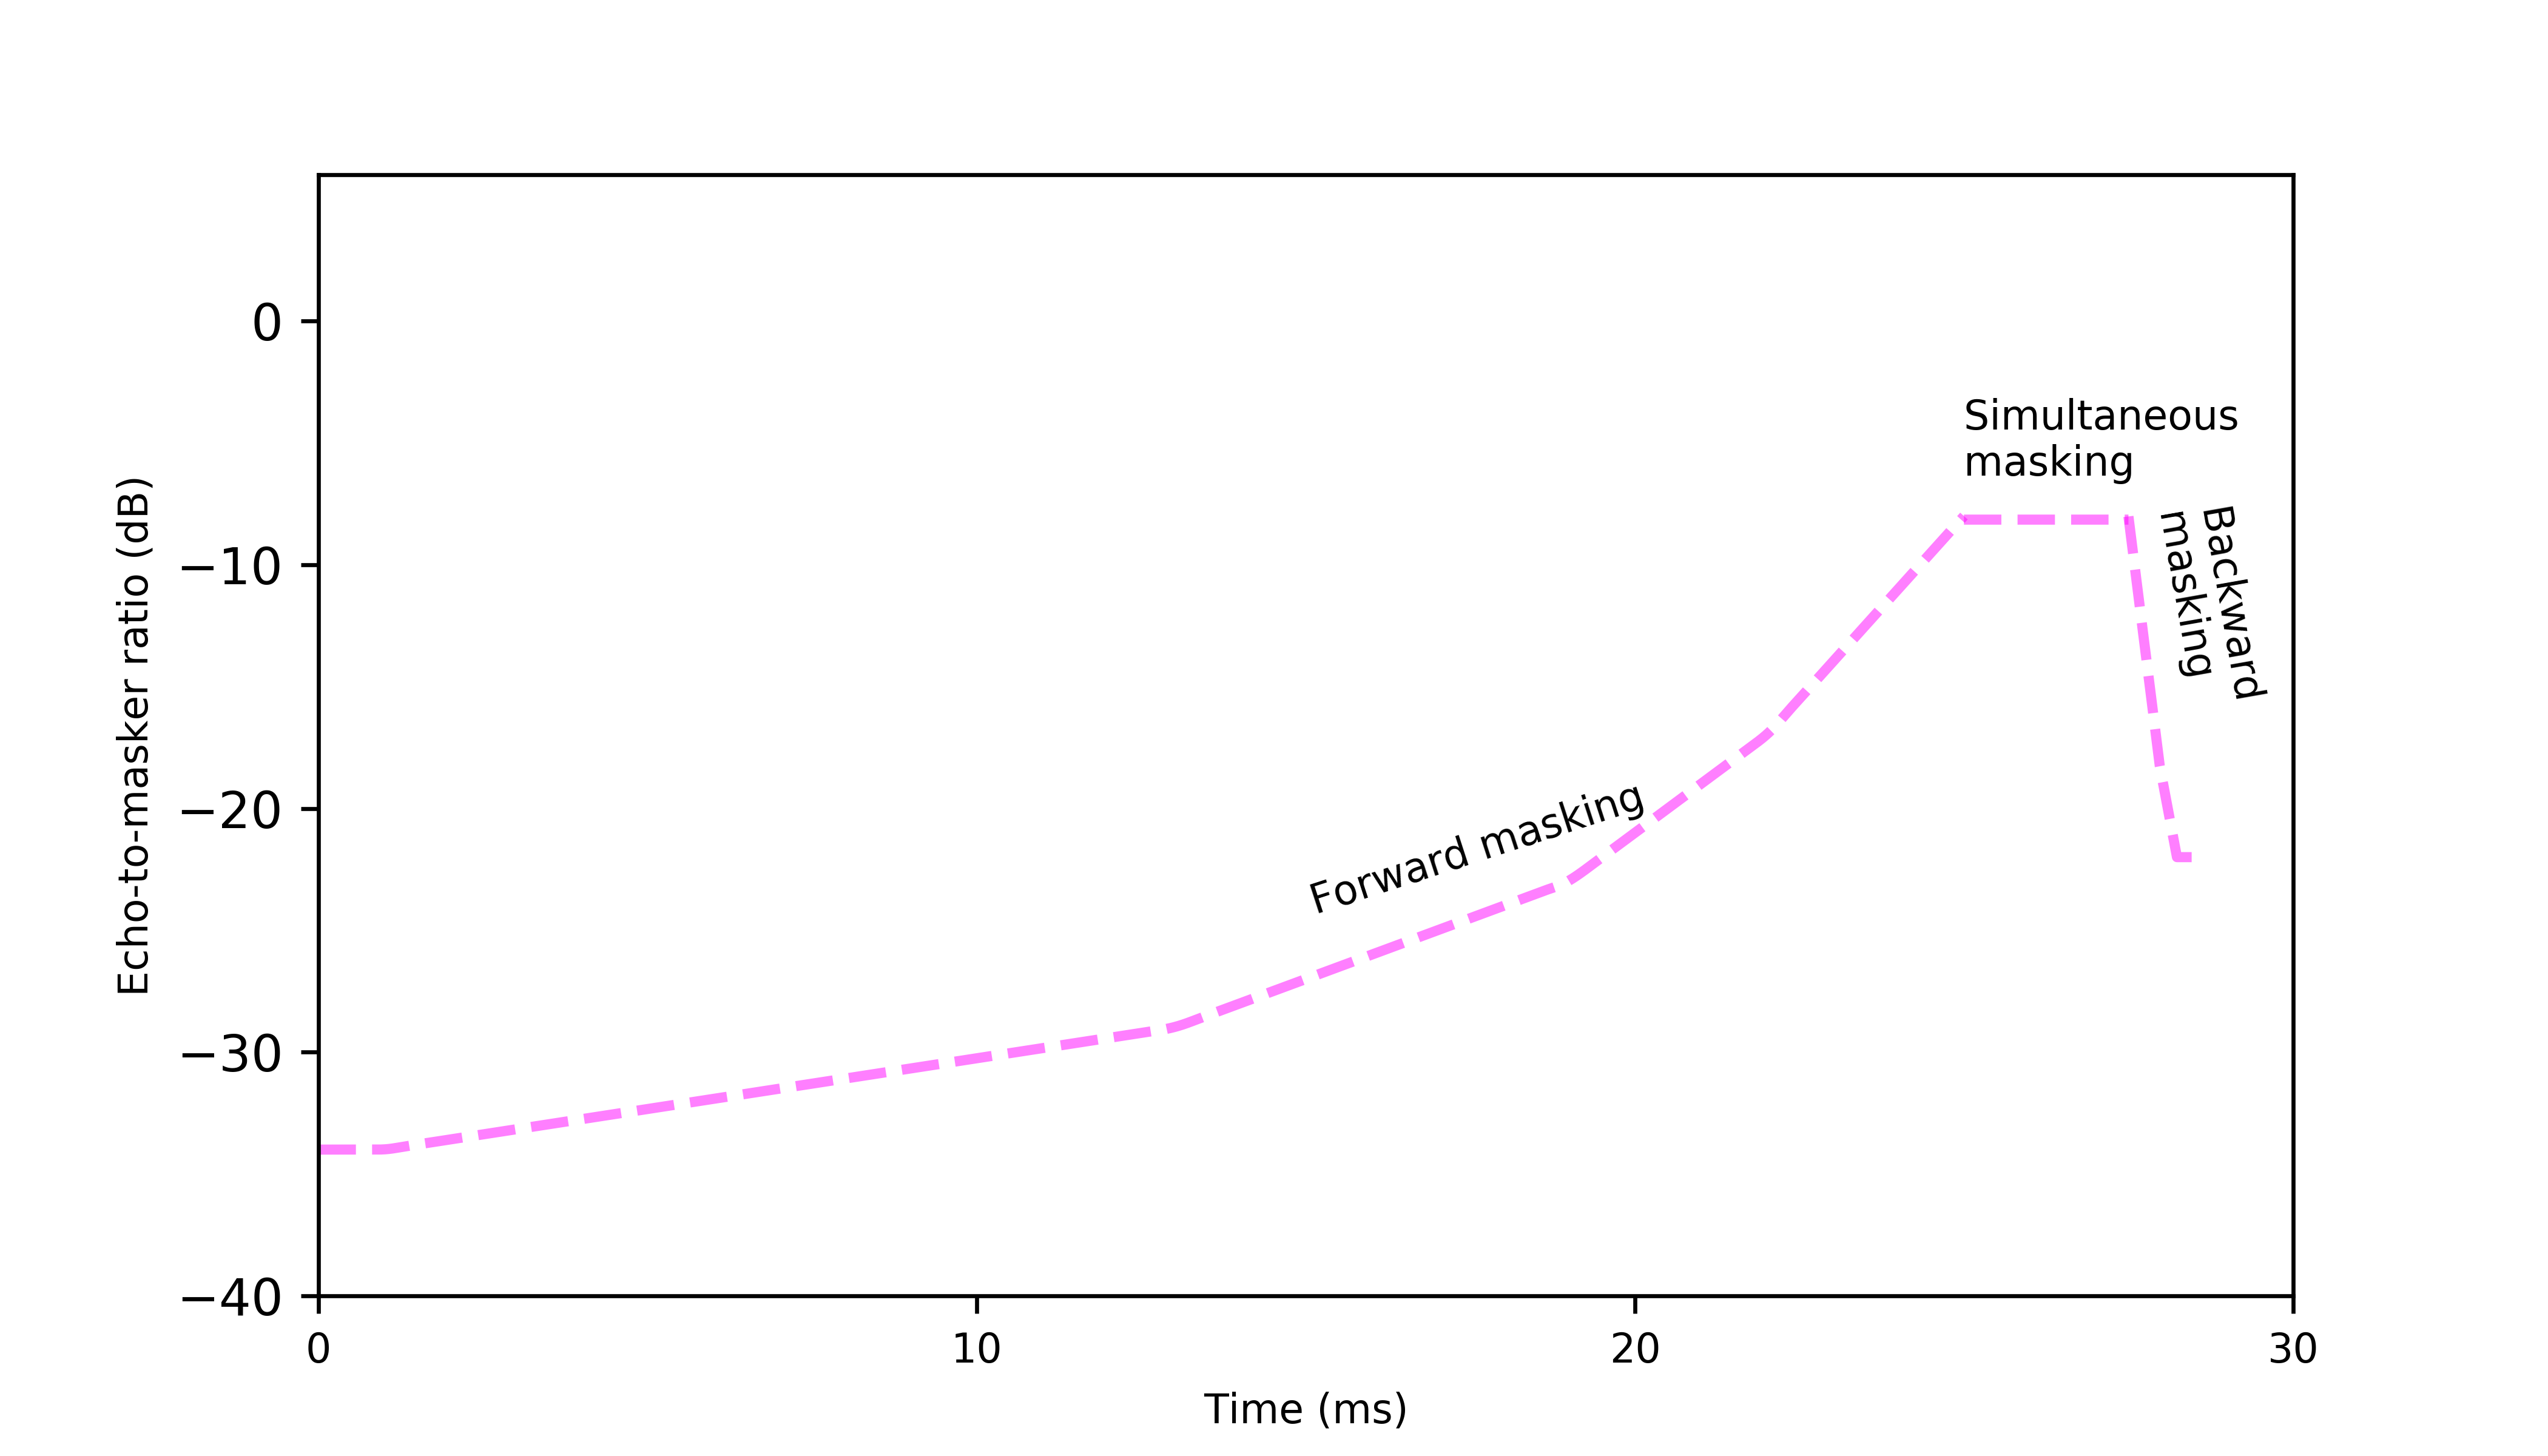
\includegraphics[]{original_papers/CPN_figures/Figures_SI/Figure_S1.png}
\centering
\caption{ The 'temporal masking envelope' used to simulate temporal masking. The envelope represents the lower echo-to-masker ratios at which a bat can detect echoes for various echo-masker delays. The envelope is the equivalent of the lowest signal-to-noise ratios at which echoes can be detected over different time delays. The envelope is centered on the position of the echo, and has a long forward masking section (at times prior to the echo), and a short backward masking section (at times after the echo). The simultaneous masking region is equal to the length of the echo itself. If the echo-to-masker ratio profile is above the temporal masking envelope for most of its duration (i.e., the echo-to-masker SPL ratio was higher than required for echo detection), we considered an echo to be heard. If the echo-to-masker ratio profile is below the envelope for more than 25$\%$ of the echo's duration, the echo was considered not heard. Here the temporal masking envelope is shown for a 2.5 ms echo. Data and sources used to construct the temporal masking envelope are given in Table 2.2}
\label{cpn_figS1}
\end{figure}

\newpage

\begin{figure}
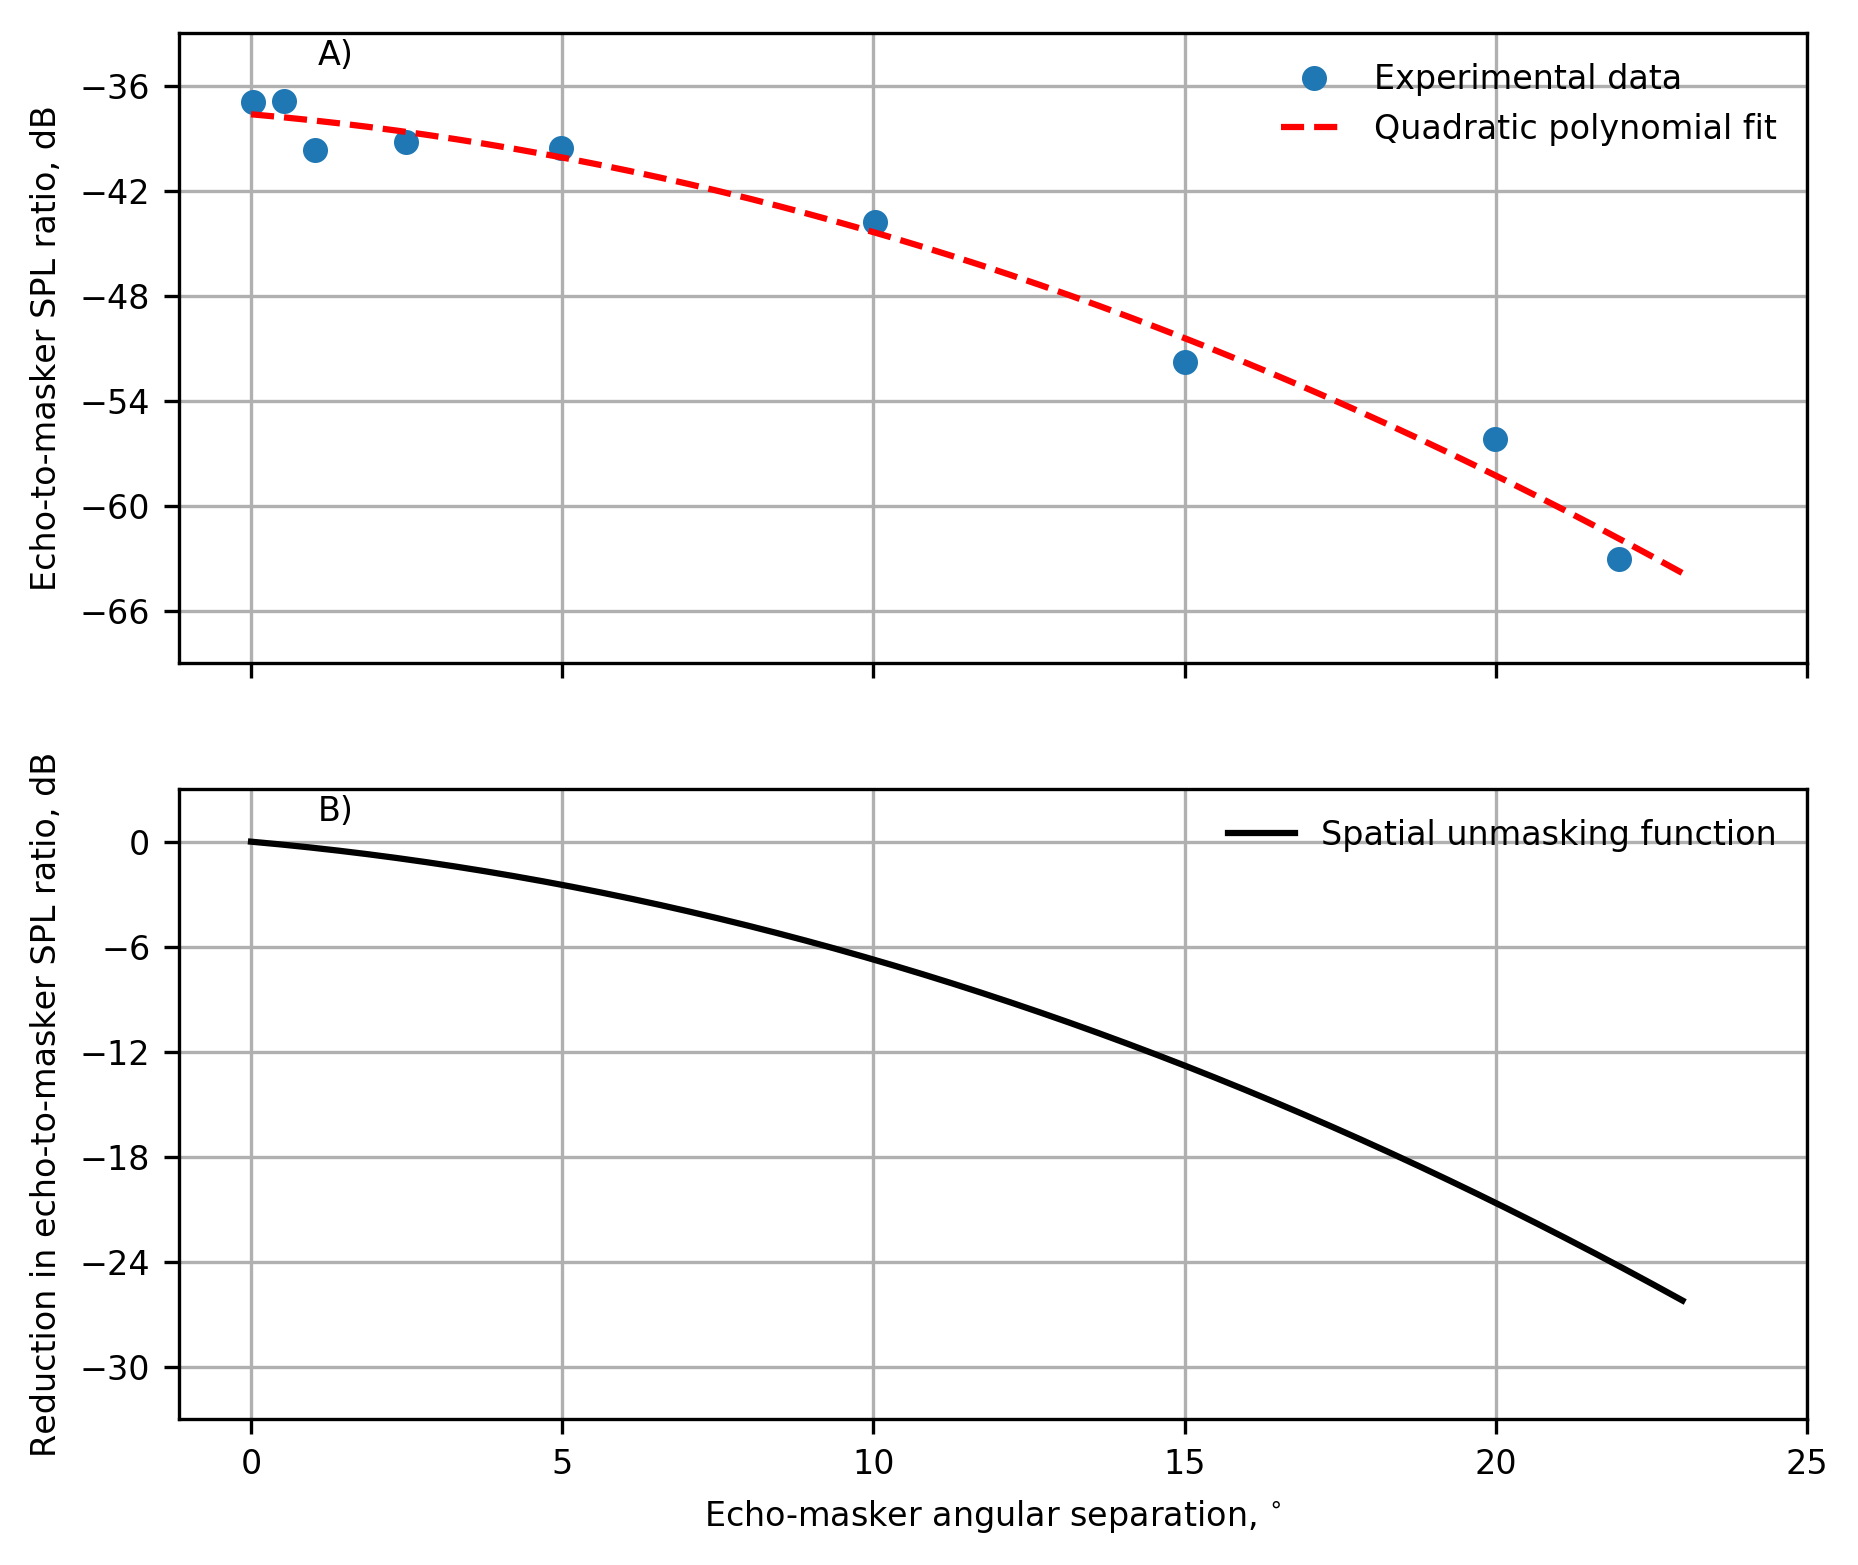
\includegraphics[]{original_papers/CPN_figures/Figures_SI/Figure_S2_2panel_exptldata_on_top.png}
\centering
\caption{The ‘spatial unmasking function’ describes the reduction in echo-to-masker SPL ratio at echo detection as a function of angular separation between echo and masker. A) The original data set of \cite{suemer2009a} (blue dot) and our digitized and
interpolated dataset (red line). The error between the data and our interpolation is less than 2 dB. B) The final spatial unmasking function as used in our simulations was derived from the interpolated fit in A), which was normalised to the echo-to-masker ratio at zero degrees angular separation. This final spatial unmasking function describes the reduction in required echo-to-masker SPL ratio relative to the co-localized case: when echo and masker are co-localized, the reduction is 0 dB, while the reduction becomes greater with increasing angular separation.}
\label{cpn_figS2}
\end{figure}

\newpage

\begin{figure}
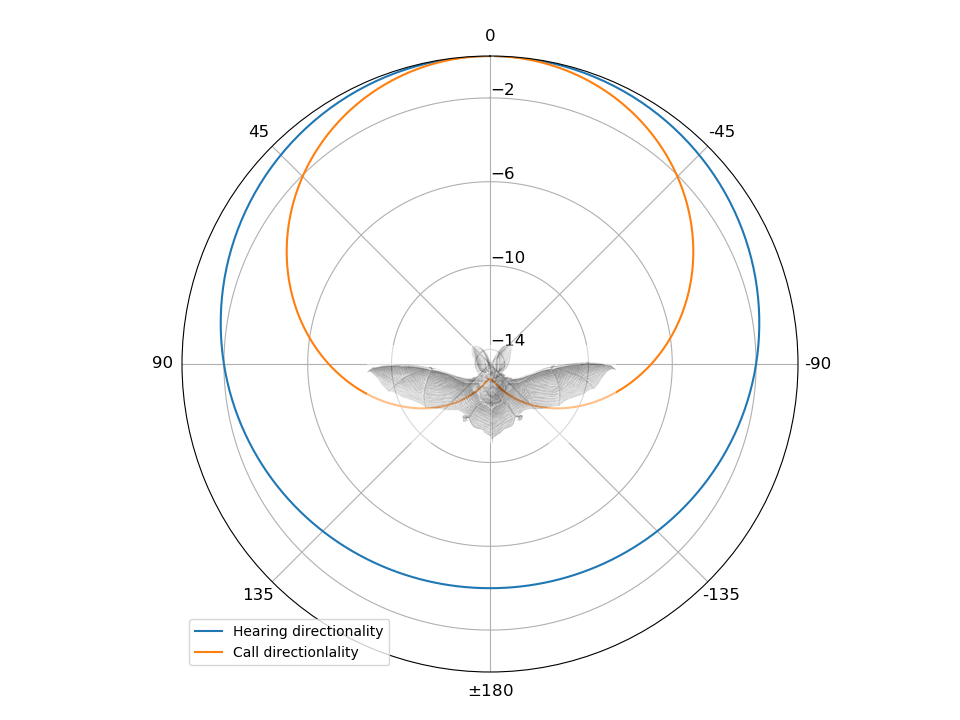
\includegraphics[]{original_papers/CPN_figures/Figures_SI/Figure_S3.png}
\centering
\caption{Calling and hearing directionality of bats. Call directionality (orange) is directional, with a difference of up to -14 dB in source level from front to back. Calls emitted to the front of a bat result in higher received levels of calls, echoes and secondary echoes. Hearing directionality (blue) is less directional, with a difference of up to -4 dB from front to back. Hearing directionality causes sounds arriving from the back to be perceived fainter than sounds arriving from the front. Bat drawing from Kunstformen der Natur (Ernst Haeckel, 1899).}
\label{cpn_figS3}
\end{figure}

\newpage

\begin{figure}
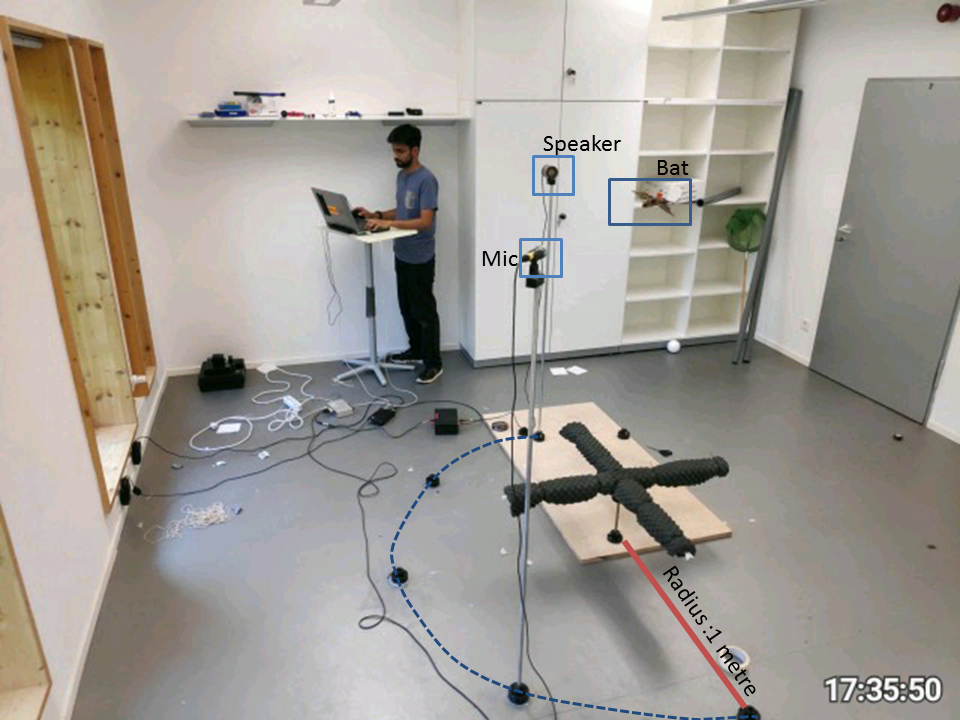
\includegraphics[]{original_papers/CPN_figures/Figures_SI/Figure_S4.png}
\centering
\caption{The ensonification setup used to measure the monostatic and bistatic target strength of a bat as an acoustic target. A stuffed \textit{Myotis myotis} bat was hung at the same height as the speaker and microphone. The bat could be rotated in the azimuth. The microphone and speaker were placed at 1 m radius around the bat at various positions (black rounded plastic molds on floor) with a separation of 45° from each other. By a combination of bat orientation, microphone and speaker positions all possible incoming and outgoing relative angles were measured. Here the positions of the speaker and microphone for a bistatic target strength measurement with 135° angle between microphone and speaker are shown.}
\label{cpn_figS4}
\end{figure}

\newpage

\begin{figure}
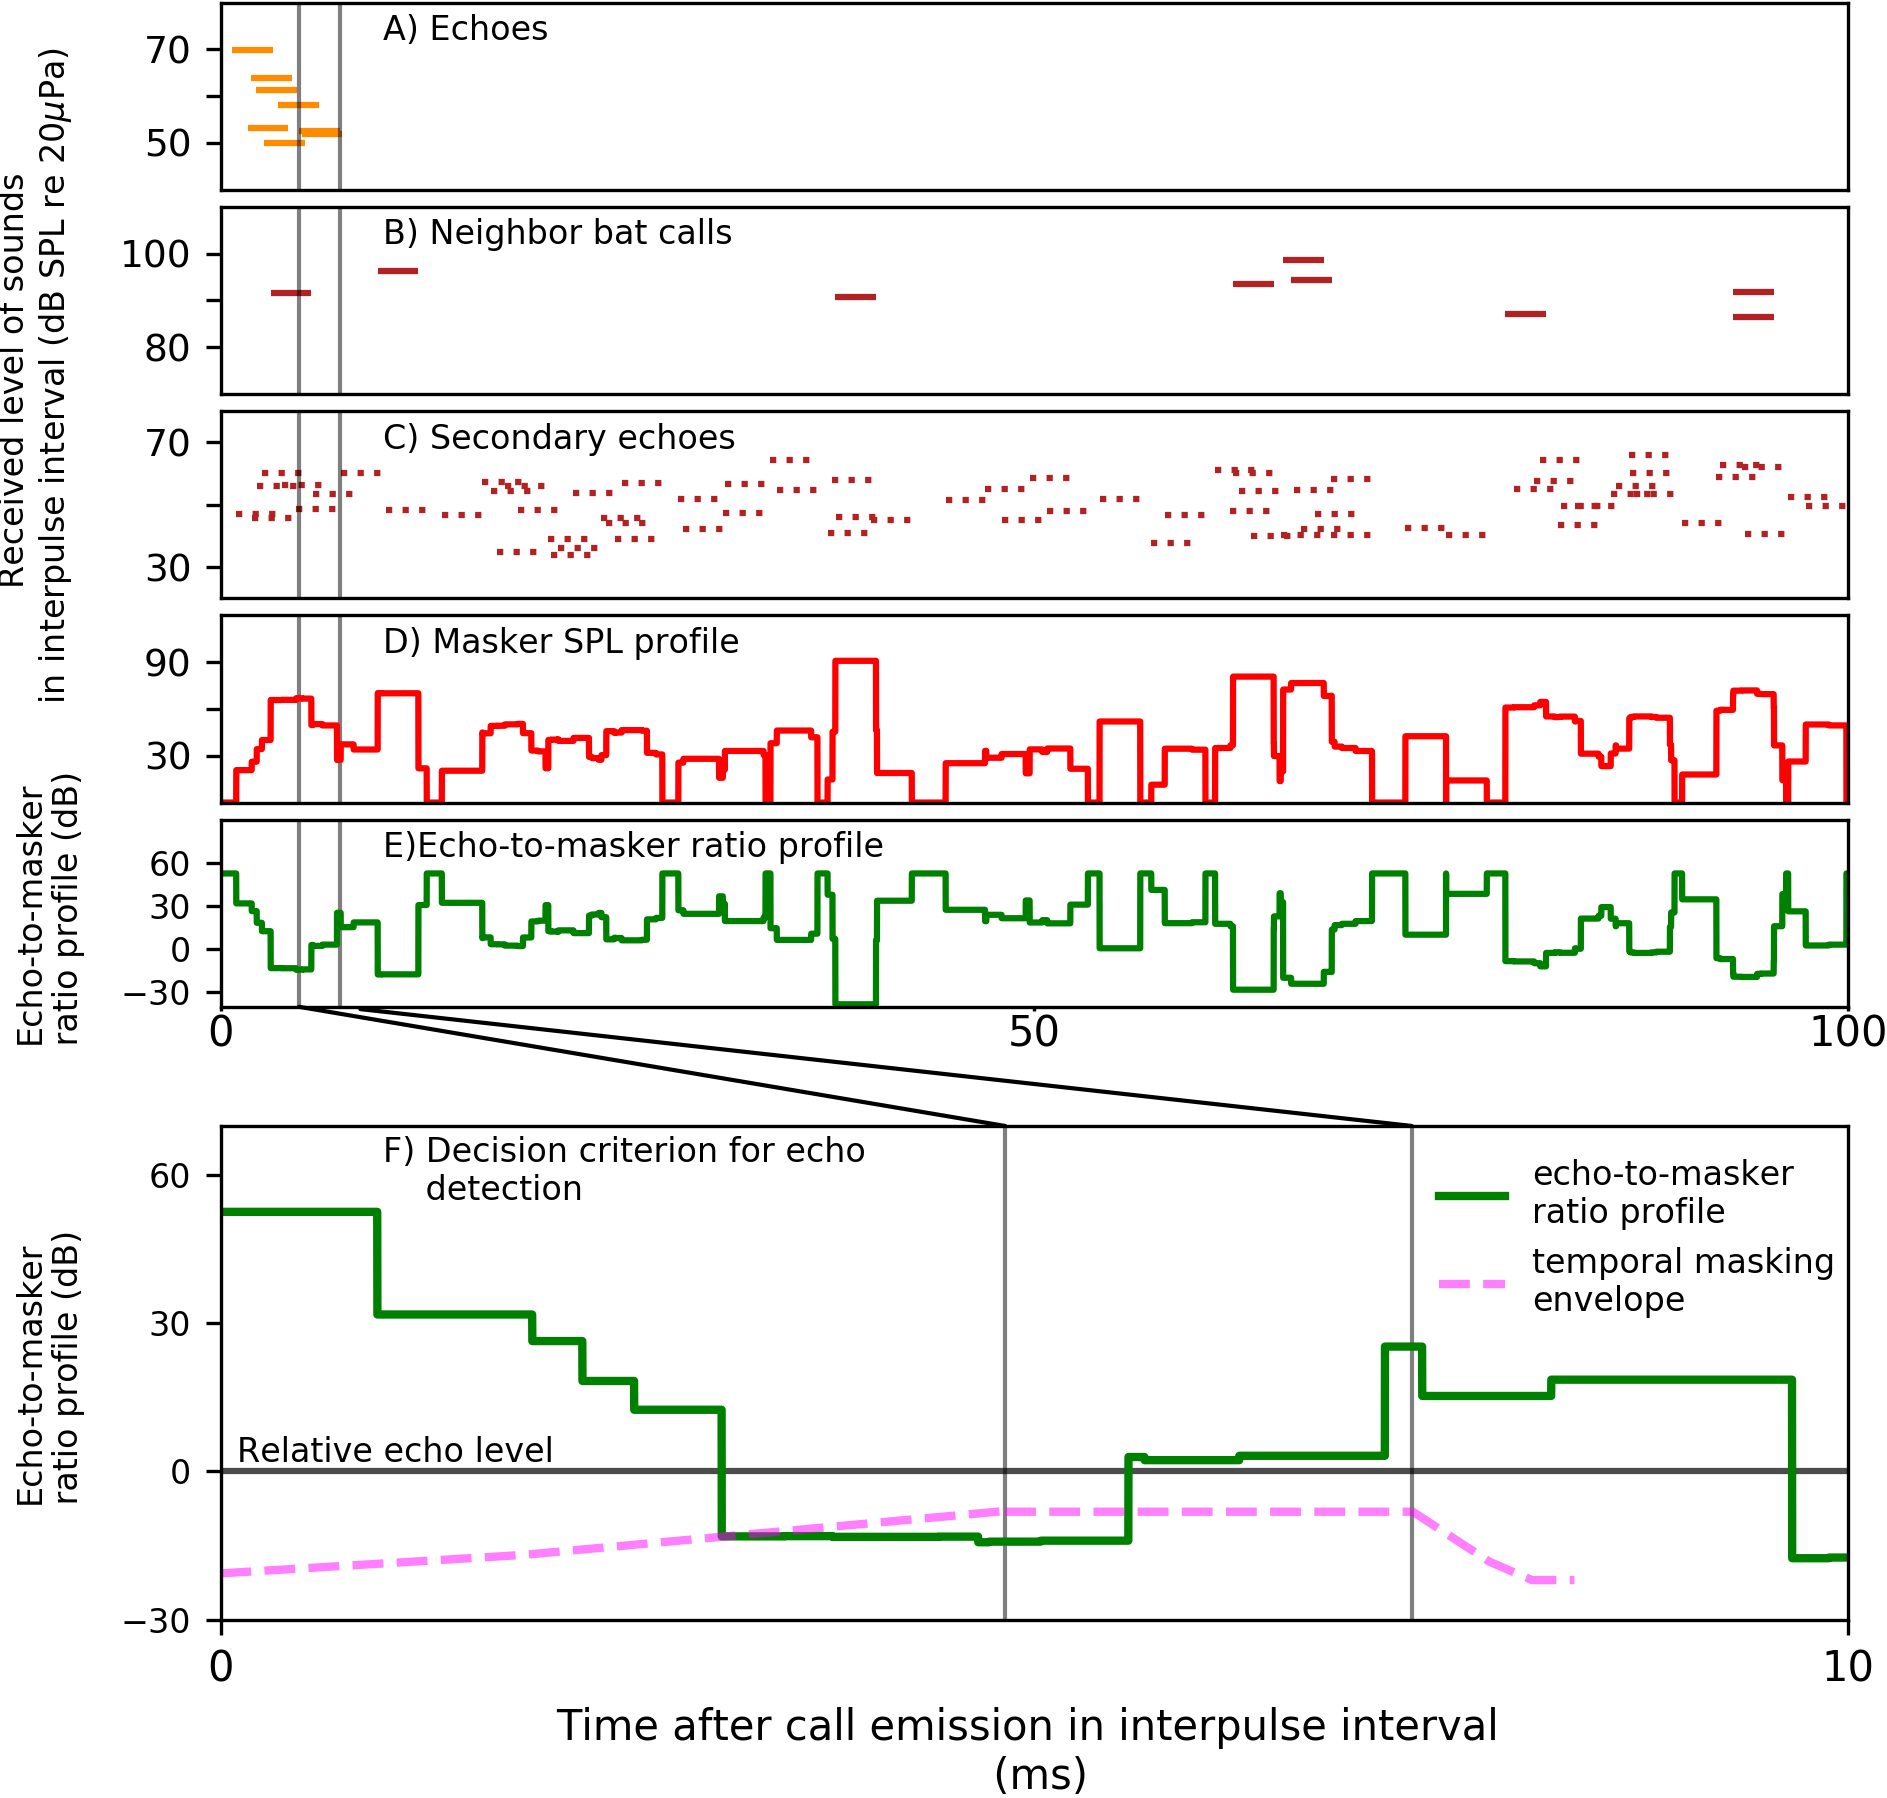
\includegraphics[]{original_papers/CPN_figures/Figures_SI/Figure_S5.png}
\centering
\caption[caption1]{Schematic representation of the sounds arriving in the interpulse interval for a simulation with a group of 10 bats (A-C) and how echo detection was determined (D-F). A-E show the full interpulse interval of 100 ms, while F shows an enlargement of the first 10 ms.  A) Timing and received SPL of the individual echoes reflected off neighbors. The echoes arrive at delays corresponding to the neighbors’ distance from the focal bat. The vertical lines single out one specific target echo to illustrate the simulated auditory system (see F). B) Timing and received SPL of the calls from neighboring bats arriving randomly with a uniform probability over the interpulse interval. C) Timing and received SPL of the secondary echoes in the interpulse interval, arriving randomly with uniform probability over the interpulse interval. D) The masker SPL profile obtained by adding the effective masker SPL of all maskers (calls and secondary echoes) over time for the chosen echo. The effective masker SPL is the received SPL corrected for spatial unmasking based on the angular separation between the echo and the masker, using the spatial unmasking function in Fig. S2. E) The echo-to-masker ratio profile obtained by normalizing the echo SPL to the masker SPL profile. 0 dB is the echo's relative SPL. F) Determining whether an echo was heard or not, by comparing the echo-to-masker ratio profile (solid green) to the temporal masking envelope (dashed pink). If the echo-to-masker ratio is above the temporal masking envelope, then the echo was not masked. In contrast, if the echo-to-masker ratio is cumulatively below the temporal masking envelope for more than 25$\%$ of the echo's duration (of 1 or 2.5 ms), then the echo was considered masked. The vertical lines indicate the actual temporal location of the example echo from A). The temporal masking envelope is centered on the chosen echo. Here, the echo-to-masker ratio is below the temporal masking envelope for almost a whole echo duration, meaning that this echo was masked.
}
\label{cpn_figS5}
\end{figure}

\hypertarget{horseshoe-bat-craziness-paper}{%
\chapter{Horseshoe bat craziness paper}\label{horseshoe-bat-craziness-paper}}

Here we describe a whole series of crazy experiments and results with horseshoe bats.

\hypertarget{ushichka}{%
\chapter{ushichka}\label{ushichka}}

Some \emph{significant} applications are demonstrated in this chapter.

\hypertarget{example-one}{%
\section{Example one}\label{example-one}}

\hypertarget{example-two}{%
\section{Example two}\label{example-two}}

\hypertarget{robust-self-calibration-of-constant-offset-time-difference-of-arrival}{%
\chapter{Robust Self-Calibration of Constant Offset Time-Difference-of-Arrival}\label{robust-self-calibration-of-constant-offset-time-difference-of-arrival}}

\chaptermark{Self-calibration of time-difference-of-arrival}

This chapter was published as a peer-reviewed paper in the conference proceedings of the International Conference on Acoustics, Speech, and Signal Processing:

\emph{Batstone, K., Flood, G., Beleyur, T., Larsson, V., Goerlitz, H. R., Oskarsson, M., \& Åström, K. (2019, May). Robust self-calibration of constant offset time-difference-of-arrival. In ICASSP 2019-2019 IEEE International Conference on Acoustics, Speech and Signal Processing (ICASSP) (pp.~4410-4414). IEEE.}

\newpage

\hypertarget{sfsabstract}{%
\section*{Abstract}\label{sfsabstract}}
\addcontentsline{toc}{section}{Abstract}

In this paper we study the problem of estimating receiver and sender positions from time-difference-of-arrival measurements, assuming an unknown constant time-difference-of-arrival offset. This problem is relevant for example for repetitive sound events. In this paper it is shown that there are three minimal cases to the problem. One of these (the five receiver, five sender problem) is of particular importance. A fast solver (with run-time under \(4~ \mu s\)) is given. We show how this solver can be used in robust estimation algorithms, based on RANSAC, for obtaining an initial estimate followed by local optimization using a robust error norm. The system is verified on both real and synthetic data.

\newpage

\hypertarget{introduction}{%
\section{Introduction}\label{introduction}}

The problem of estimating receiver-sender node positions from measured arrival times of radio or sound signals is a key issue in different applications such as microphone array calibration, radio antenna array calibration, mapping and positioning. This field is well researched but in this paper we will focus on the anchor-free sensor network calibration both in terms of time-of-arrival measurements (TOA) and time-difference-of-arrival measurements (TDOA).
For time-of-arrival the planar case of three receivers and three senders (3R/3S) was solved in \cite{stewenius-phd-2005}.
For the full 3D case the over-determined problem (10R/4S) was studied in \cite{pollefeys-nister-icassp-08}, where a solver for this non-minimal case was provided. There are actually three minimal cases for the 3D case, namely (4R/6S), (5R/5S) and (6R/5S). A practical solver was presented in
\cite{kuang-burgess-etal-icassp-13}. There are in general \(38\), \(42\) and \(38\) solutions respectively for the three different set ups.
Faster solvers for these minimal cases were provided in \cite{larsson2017polynomial}.

In this paper we study the constant offset TDOA self-calibration problem. It is a problem that naturally arises e.g.~when signals are emitted with a known period. As an estimation problem it lies between TOA and full TDOA. In the paper we study the minimal (5R/5S) problem and provide a fast (few \(\mu s\)) solver.
Robust parameter estimation often use the hypothesize and test paradigm, e.g.~using random sampling consensus, \cite{fischler-bolles-ca-81} or one of its many variants (\cite{chum2003locally,raguram2013usac,korman2018latent}). In these frameworks minimal solvers are important building blocks for generating model hypotheses, and we show in the paper how a minimal solver can be used for robust parameter estimation of sender positions, receiver positions and unknown offset. The system is capable of handling missing data, outliers and noise. The algorithms are tested on synthetic data as well as real data, in an office environment and in a cave.The methods are straightforward to generalize for degenerate configurations which arise if senders or receivers are restricted to a plane or to a line.

\hypertarget{time-difference-of-arrival-self-calibration}{%
\section{Time-difference-of-arrival self calibration}\label{time-difference-of-arrival-self-calibration}}

The problem we are considering involves \(m\) receiver positions \(\mathbf{r}_i \in \mathbb R^3\), \(i = 1, \dots, m\) and \(n\) sender positions \(\mathbf{s}_j \in \mathbb R^3\), \$ j = 1, \dots, n\$. This could for example represent the microphone positions and locations of sound emissions, respectively. Assume that the arrival time of a sound \(j\) to receiver \(i\) is \(t_{ij}\) and that the time that sound \(j\) is emitted is \(T_j\).
Multiplying the travel time \(t_{ij} - T_j\) with the speed \(v\) of the signal we obtain the distance between senders and receiver,

\begin{equation}
v (t_{ij}-T_j)   = {\norm{\mathbf{r}_i - \mathbf{s}_j}}_2 ,
\label{eq:tdoa}
\end{equation}
where \({\norm{.}}_2\) is the \ltwo-norm. The speed \(v\) is throughout the paper assumed to be known and constant.

In many settings the times of emissions \(T_j\) are unknown, but regular, \eg
\begin{equation}
T_j = k_1 j + k_0, 
\label{eq:regular}
\end{equation}
where the interval \(k_1\) is known. Inserting \eqref{eq:regular} into \eqref{eq:tdoa} we
obtain
\begin{equation}
v (t_{ij}-k_1 j - k_0)   = {\norm{\mathbf{r}_i - \mathbf{s}_j}}_2 . 
\end{equation}
Assuming an erroneous (but regular) emission time
\(\tilde{T}_j = k_1 j + \tilde{k}_0\) and
introducing (the measured) \(z_{ij} = v (t_{ij}-\tilde{T}_j)\) and (the unknown) \(o = v (k_0-\tilde{k}_0)\) yields the following expression
\begin{equation}
 z_{ij}   = {\norm{\mathbf{r}_i - \mathbf{s}_j}}_2 + o. 
\end{equation}
Note that this is a simplified variant of the general time-difference-of-arrival problem (see \eg  \cite{kuang2013stratified}), which allows for a different offset \(o\) for every \(j\),
\begin{equation}
 z_{ij}   = {\norm{\mathbf{r}_i - \mathbf{s}_j}}_2 + o_j.
\end{equation}

\noindent 

\begin{problem1} \label{prob_misstoa}
({{Constant Offset Time-Difference-of-Arrival  Self-Calibration}}) Given measurements $\tilde{z}_{ij}$ 
\vspace{-5pt}
\begin{equation}
\tilde{z}_{ij} = {\norm{\mathbf{r}_i - \mathbf{s}_j}}_2 + o  + \epsilon_{ij}, 
\label{eq:distance}
\vspace{-5pt}
\end{equation}
for a subset $W \subset I$ of all the receiver-sender index pairs $I = \{ (i,j) | i = 1, \ldots m, j = 1, \ldots, n \}$ determine receiver positions $\mathbf{r}_i$, $ i = 1, \dots, m$ and sender positions $\mathbf{s}_j$,  $j = 1, \dots, n$ and offset $o$. 
Here the errors $\epsilon_{ij}$ are assumed to be either 
{\bf inliers}, in which case the errors are small ($\epsilon_{ij} \in N(0,\sigma)$) or {\bf outliers}, in which case the measurements are way off. 
\end{problem1}

Here we will use the set \(\Win\) for the indices \((i,j)\) corresponding to the inlier measurements and \(\Wout\) for the indices corresponding to the outlier set.
\vspace{-5pt}

\section{Local optimization and the low~rank~relaxation}
\label{sec:rank}
\vspace{-5pt}

If an initial estimate of the parameters \(\theta_1 = \{ R, S, o \}\) is given and if the set of inliers is known, then refinement of the estimate can be found by optimization methods, \eg Levenberg-Marquardt (LM) (\cite{levenberg1944method,marquardt1963algorithm}),
\begin{equation}
\min_{\theta_1} f(\theta_1) = \sum_{(i,j) \in \Win} (z_{ij} - ( {\norm{\mathbf{r}_i - \mathbf{s}_j}}_2 +o) )^2 .
\end{equation}

There is an interesting relaxation to the problem, that exploits the fact that the matrix with elements \((z_{ij}-o)^2\) is rank \(5\), (\cite{pollefeys-nister-icassp-08}). Further simplifications use the double compaction method (\cite{kuang2013stratified}). The double compaction matrix \(M\) is defined as the matrix with elements
\begin{equation}
M_{ij}=(z_{ij}-o)^2 -a_i-b_j,
\label{eq:dc}
\end{equation}
and it can be shown to have rank \(3\), i.e.~\(M = U^T V\), where \(U\) is of size \(3 \times m\) and \(V\) is of size \(3 \times n\).
The relaxed problem involves a set of parameters
\(\theta_2 = \{ U, V, b, a, o \}\). Here the constraints can be written as
\begin{equation}
z_{ij} =  \sqrt{u_i^T v_j + a_i + b_j} + o ,
\end{equation}
where \(u_i\) denotes column \(i\) of \(U\) and \(v_j\) denotes column \(j\) of \(V\).
Refinement of parameters can be done by performing local optimization on
\begin{equation}
\min_{\theta_2} f(\theta_2) = \sum_{(i,j) \in \Win} \left ( z_{ij} - ( \sqrt{u_i^T v_j + a_i + b_j} + o ) \right )^2 .
\label{eq:relaxed}
\end{equation}

\vspace{-5pt}
\section{Minimal problems and solvers}
\label{sec:minimal}
\vspace{-5pt}

By counting equations and unknowns, one finds that there are three minimal problems. The first two are the symmetric case when \(m=4, n=7\) or \(m=7, n=4\). This case is not addressed in this paper, but we believe it to be difficult to solve. The other case is \(m=n= 5\). Here, we first present a solver for the constant offset and then discuss how to solve for sender and receiver positions.

Given a \(5 \times 5\) matrix, \(Z\), with time-difference-of-arrival measurements \(z_{ij}\), the rank \(3\) constraint on the double compaction matrix in \eqref{eq:dc}
can be written as
\begin{equation}
f(o) = \det ( C^T (Z-o)^{\circ 2} C )  = 0, 
\end{equation}
where
\begin{equation}
C = \begin{pmatrix}
-1 & -1 & -1 & -1\\
1 & 0 & 0 & 0\\
0  & 1 & 0 & 0\\
0 & 0 & 1 & 0 \\
0 & 0 & 0 & 1 
\end{pmatrix} 
\end{equation}
and \(^{\circ 2}\) denotes element-wise squaring (Hadamard power).
Although the elements of \((Z-o)^{\circ 2}\) are of degree 2 in \(o\), the quadratic terms cancel out after multiplication with \(C^T\) and \(C\). Thus the elements of \(C^T (Z-o)^{\circ 2} C\) are linear in \(o\).
Since the determinant is linear in each column, the determinant \(f(o)\) is a polynomial of degree four in the offset \(o\). This can be summarized as

\begin{theorem}
Given time-difference-of-arrival measurements from five receivers to five senders, there are four possible offsets $o$, given as the roots to the fourth degree polynomial $f(o)$, counting complex roots and multiplicity of roots. 
\end{theorem}

For each solution \(o\) it is possible to generate a solution \(\theta_2\) to the relaxed problem,
according to

\begin{equation*}
\! b \! = \! \begin{pmatrix} (z_{11} \! - \! o)^2  \! \!  &  \! \!  (z_{12}-o)^2  \! \!  &  \! \!  (z_{13}-o)^2 \! \!  &  \! \!   (z_{14}-o)^2 \! \!  &  \! \!   (z_{15}-o)^2 \end{pmatrix} \! ,
\end{equation*}
\begin{equation}
a =  \begin{pmatrix} 0 \\ (z_{21}-o)^2 -(z_{11}-o)^2\\ (z_{31}-o)^2 -(z_{11}-o)^2 \\ (z_{41}-o)^2 -(z_{11}-o)^2 \\ (z_{51}-o)^2 -(z_{11}-o)^2 \end{pmatrix},
\end{equation}
\begin{equation}
U =  \begin{pmatrix} 0 & u_2 & u_3 & u_4 & u_5\end{pmatrix}, 
\end{equation}
\begin{equation}
V =  \begin{pmatrix}0 & v_2 & v_3 & v_4 & v_5\end{pmatrix} ,
\end{equation}
where \(\begin{pmatrix}u_2 & u_3 & u_4 & u_5\end{pmatrix}^T \begin{pmatrix} v_2 & v_3 & v_4 & v_5\end{pmatrix}\) is any rank \(3\) factorization of the matrix \(C^T (Z-o)^{\circ 2} C\).

From a solution \(\theta_2\) to the relaxed problem it is possible to upgrade to a solution \(\theta_1\) to the original problem. This involves solving a system of polynomial equations. The procedure was first described in \cite{kuang-burgess-etal-icassp-13}, where an algorithm for solving this was presented. Recently, a faster algorithm was presented in \cite{larsson2017polynomial}.

An efficient implementation for calculating the four solutions of the offset \(o\) given the measurements \(z\) takes \(4~ \mu s\) for a C++-implementation. Generating the solution \(\theta_2\) to the relaxed problem adds a few \(\mu s\). However, calculating a solution \(\theta_1\) to the original problem takes another \(22 ~ms\). Thus, it is advantageous to estimate the parameters of the relaxed problem and postpone the upgrade from \(\theta_2\) to \(\theta_1\) as a final step, see Table \ref{Tabletime}.

\begin{table}
\caption{Execution times for $5 \times 5$ minimal solvers steps. Notice that the steps of calculating $o$ and the relaxed solution is significantly faster than upgrading to the full solution}
\centering
\vspace{4mm}
\begin{tabular}{@{}ccc@{}} \toprule
%& \multicolumn{5}{c}{CS (dB)} & \multicolumn{5}{c}{SSIM} \\ \cmidrule(r){2-11}
Implementation & Matlab  & C++ \\
\midrule 
Calculation of $o$ & $38 \, \mu s$ & $3.7 \, \mu s$ \\
Calculation of $\theta_2 = \{ U,V,a,b,o \}$ & $100 \, \mu s$ & N/A \\
Calculation of $\theta_1 = \{ R,S,o \}$ & $600 \, ms$ & $22 \, ms$ \\
\bottomrule
\end{tabular}
\label{Tabletime}
\end{table}

\vspace{-5pt}

\section{Using RANSAC for five rows}
\label{sec:ransac}
\vspace{-5pt}

We propose the use of the fast minimal solver in an hypothesize and test framework to obtain (i) a initial estimate on the offset \(o\) and (ii) an initial inlier set. The steps are described in Algorithm\textasciitilde{}\ref{a_offset}

\begin{algorithm}
\caption{Offset RANSAC}\label{a_offset}
\begin{algorithmic}[1]
\State Randomly select $5$ rows and columns. Find the four solutions on $o$ given the time-difference-of-arrival measurements. 
\State For each solution $o$, calculate the relaxed solution $\theta_2 = \{ U,V,a,b,o \}$.
\State For selected rows and for each remaining column, check for inliers according to the residuals in \eqref{eq:relaxed}.
\end{algorithmic}
\end{algorithm}

\vspace{-5pt}
\section{Robust estimation of parameters}
\label{sec:ransac}
\vspace{-5pt}

We use these minimal solvers with RANSAC as described in the previous section to find one or several initial estimates of the parameters \(\theta_2\) for a subset of five receivers and \(k\) senders. The solution is extended to additional rows and/or columns using robust techniques as described in \cite{batstone2016robust}. During this process it is useful to keep the errors down by occasionally refining the solutions using local optimization. This has shown to reduce failures, see e.g.~(\cite{engels-stewenius-etal-06,klein2007parallel}).
In the proposed estimation algorithm we postpone the upgrade from \(\theta_2\) to \(\theta_1\) until we have found a good solution involving a large portion of the receiver and sender positions.
\vspace{-5pt}

\section{Experimental Validation}
\label{sec:exp}
\vspace{-5pt}
\subsection{Minimal Solver}
\vspace{-5pt}

To test the numerical accuracy and robustness of our minimal solver we conducted an experiment using simulated data without noise. We generated a large number of instance problems (10,000) with known offsets. We then ran our solvers and compared the returned solutions with the ground truth solution. For each instance problem we recorded the distance to the closest solution. In Figure \ref{fig:f_hist} the resulting histogram of the logarithm of the absolute errors are shown. As can be seen, both implementations get close to machine precision.

\begin{figure}
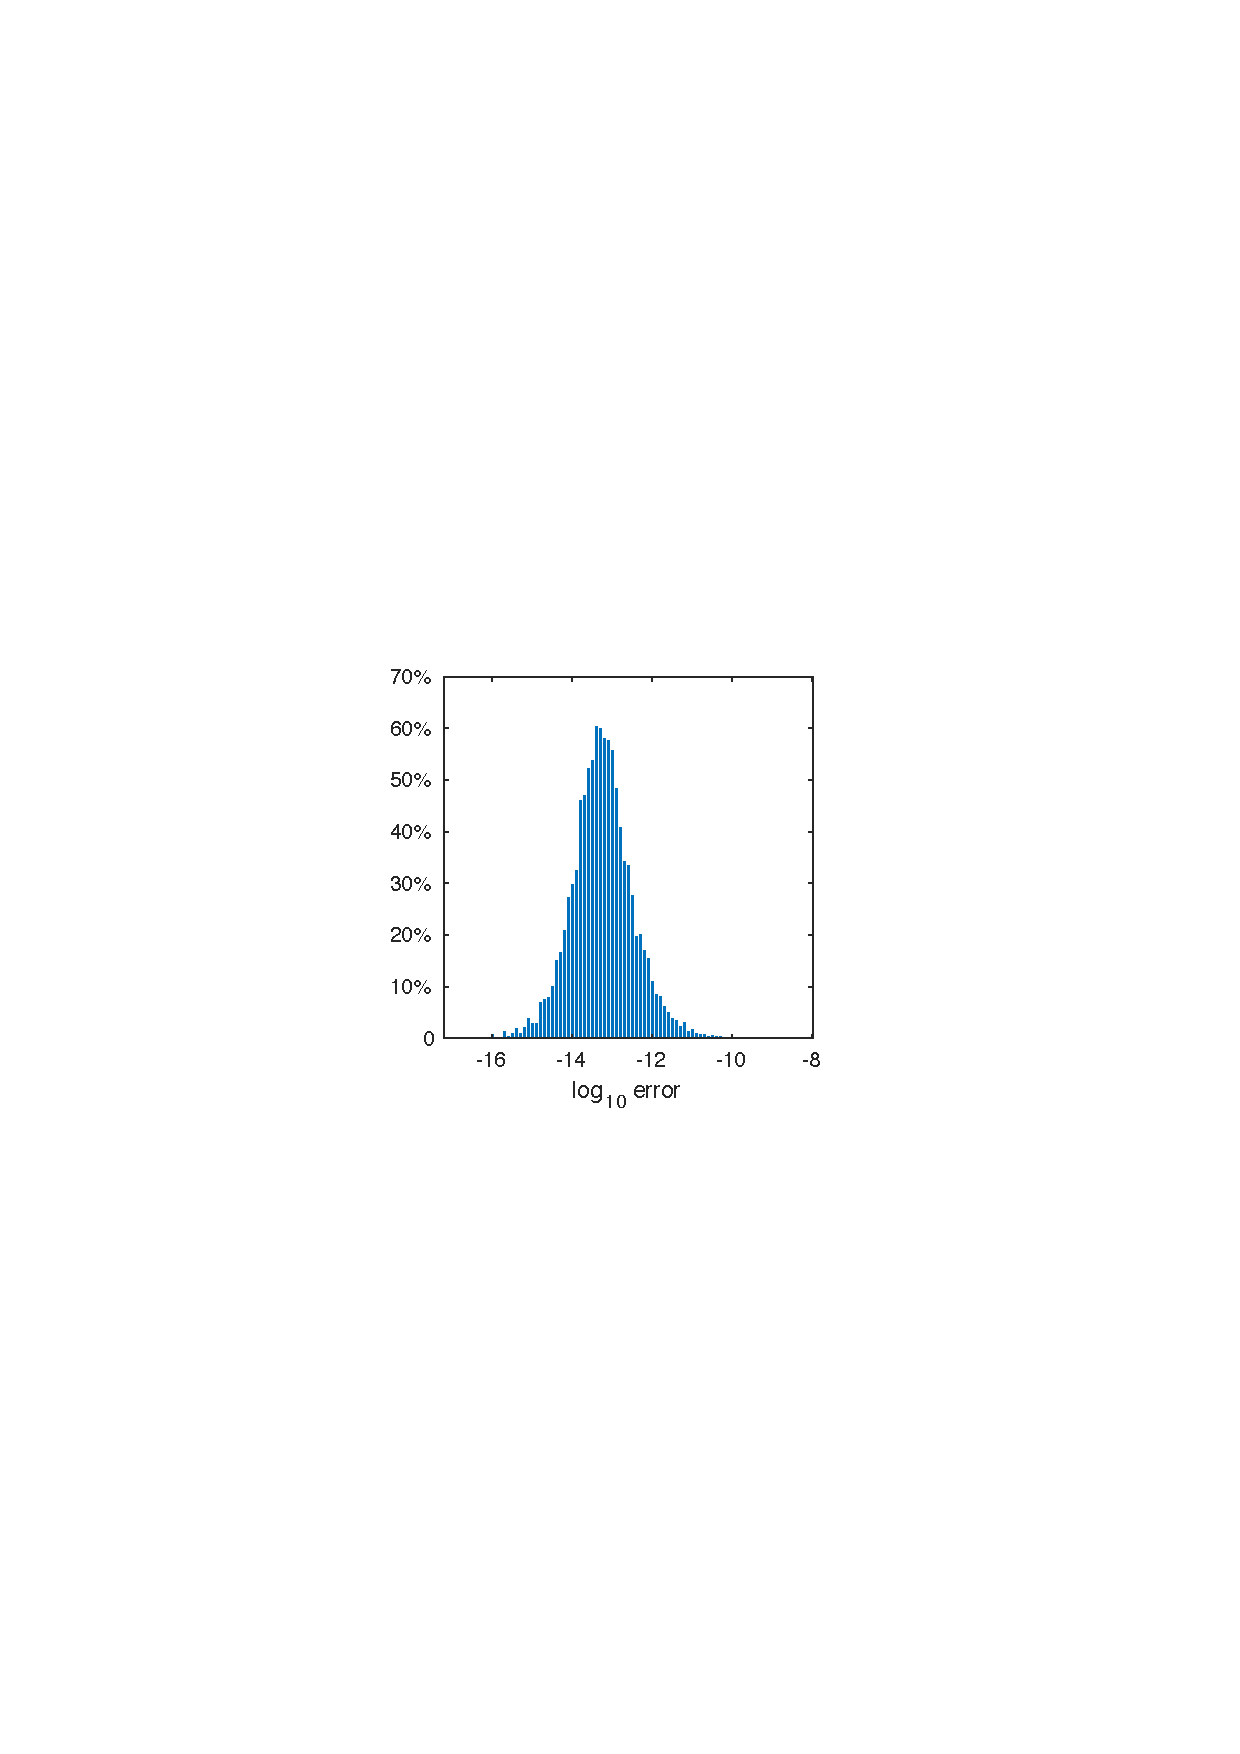
\includegraphics[width=0.4\textwidth]{original_papers/icassp_2018/figs/hist_matlabsolver.pdf}
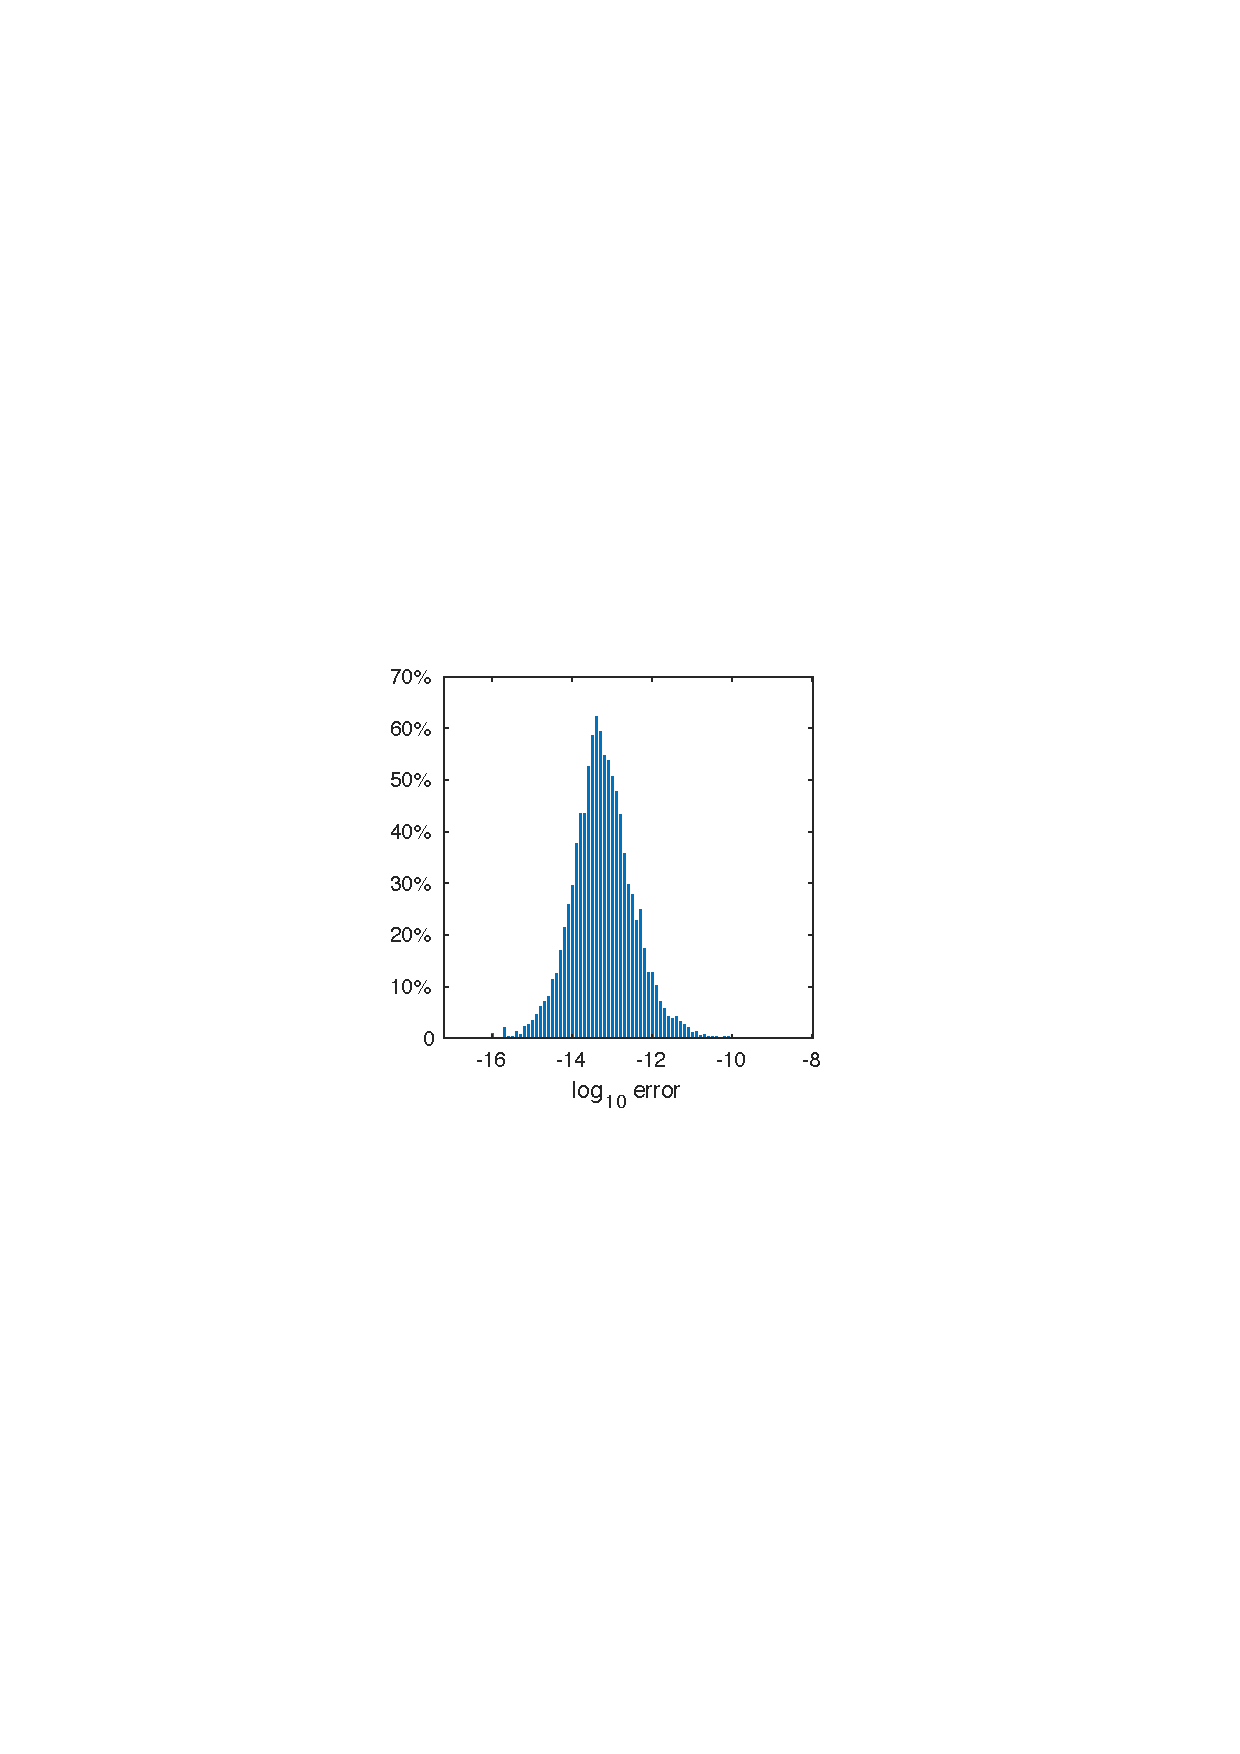
\includegraphics[width=0.4\textwidth]{original_papers/icassp_2018/figs/hist_mexsolver.pdf}
\caption{Left shows the histogram of the logarithm of the absolute errors, for the Matlab implementation of our minimal solver. To the right the corresponding histogram for the C++ implementation.}
\label{fig:f_hist}
\end{figure}

\vspace{-5pt}
\subsection{Experimental Setup for Real Data}
\vspace{-5pt}

We have tested our system on (i) experiments made in an office environment and (ii) experiments made at the Orlova Chuka cave, Bulgaria.

For the office experiments, 12 microphones (8x t.bone MM-1, 4x Shure SV100) were positioned around a room (\(\sim 3 \times 5~m^2\)) and measured using a laser to obtain ground truth positions of the microphones with an error of \(\pm 2~ mm\). The space was cleared of most the furniture to create an open space to conduct the experiment in. The sound recordings were captured using a Roland UA-1610 Sound Capture audio interface and automatically amplified. The recordings were made using the open source software Audacity 2.3.0 with a sampling frequency of \(96~kHz\) on a laptop. A synthetically generated chirp was then played using a simple loudspeaker every half second for \(30~s\) while moving the speaker around in the room.

For the cave experiments, 12 microphones (4x Sanken CO-100K, 8x Knowles SPU0410) were positioned in a section of the cave, four microphones were placed on an inverted T array near one wall, while the other eight microphones were placed on the adjacent wall. The sound recordings were captured using pre-amplifiers (Quadmic, RME) and two synchronised Fireface 800 (RME) audio interfaces running at a sampling frequency of \(192 ~kHz\). Recording and playback were controlled via a custom written script based on the sound device library
(\cite{geier2015}) in Python 2.7.12 (\cite{van1995python}). Ultrasonic chirps (\(8~ms\), \(16-96~kHz\) upward hyperbolic sweep) were played every second via one of the audio interfaces, amplified (Basetech AP-2100) and presented through a Peerless XT25SC90-04 loudspeaker. The speaker was attached to a 3-m-long pole and slowly waved in the approximately \(5 \times 9 \times 3 ~m^3\) recording volume. Playbacks were done past 6:00 am to prevent disturbing the resident bat population.

\vspace{-5pt}
\subsection{Experimental Evaluation for Real Data}
\vspace{-5pt}

Once the office recordings were taken, an algorithm was used to find the chirps in the captured sound recordings and the algorithm then outputs the \(z_{ij}\) matrix. This can then be used in our RANSAC scheme, Algorithm\textasciitilde{}\ref{a_offset}. For this experiment we used the (5R/5S) minimal solver. A fixed number of iterations was used; 100 iterations for the initial selection of 5 receivers and senders, then the extension to more columns and rows was allowed until there was no better solution. The tolerance was set to \(T=0.01\) for the initial selection and extension of rows and column.

Once the initial values have been estimated, it underwent \(l^{2}\) optimization on the inlier set. The results of the estimated microphone positions after the optimization are shown in Figure \ref{f_454H}.

This produced an Euclidean distance error between each of the microphones calculated position and its ground truth position as 0.2016,0.0587,0.1444,0.1153,0.2017, 0.1326,0.1407, 0.1198,0.2041,0.2010,0.1908,0.2110) m.

For graphical purposes, a Procrustes fitting was used on the microphone positions to spread the total error over all 12 microphones. In the Procrustes fitting only rotation and translation were allowed.

For the cave experiment a similar scheme was devised and the results are shown in Figure \ref{f_bat}.

\begin{figure}
\begin{tabular}{c}
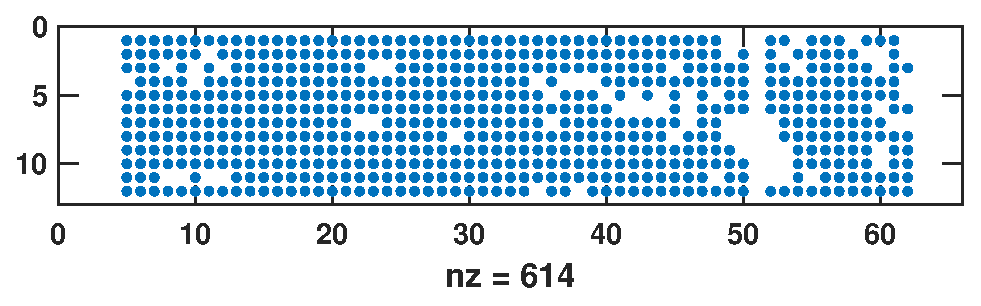
\includegraphics[width=0.8\textwidth]{original_papers/icassp_2018/figs/MH454_F_inl.eps} \\
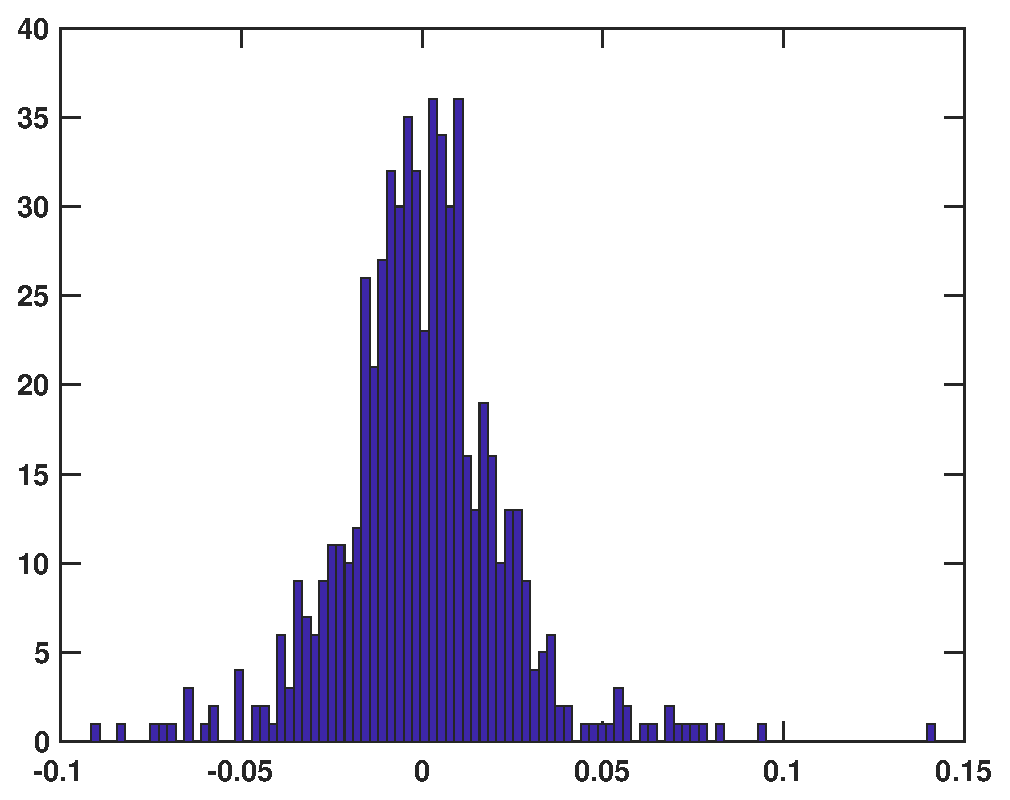
\includegraphics[width=0.4\textwidth]{original_papers/icassp_2018/figs/MH454_F_res.eps} 
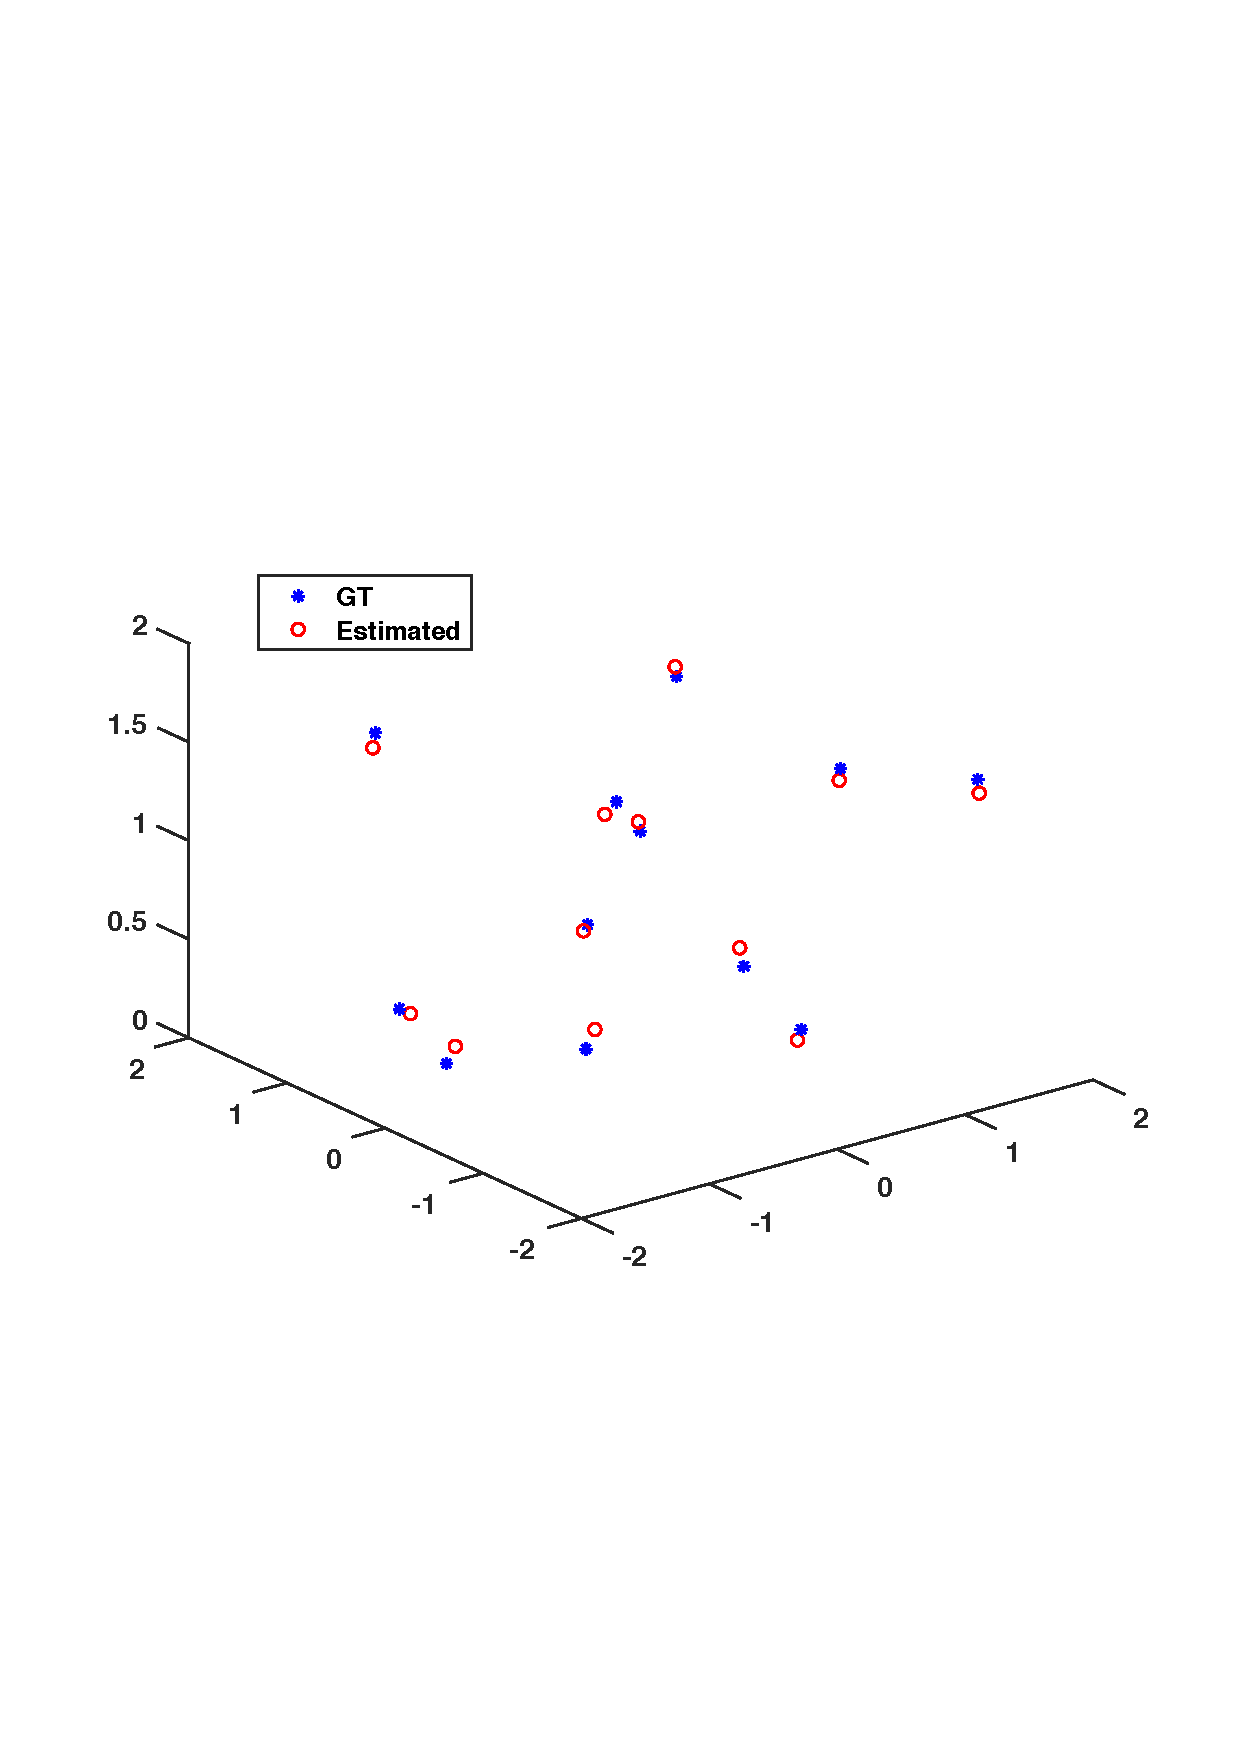
\includegraphics[width=0.4\textwidth]{original_papers/icassp_2018/figs/MH454_F_fig_new.pdf} 
\end{tabular}
\caption{For the office experiment the figure shows  detected inliers $\Win$ (top),  inlier residual histogram (bottom left), and  estimated and ground truth microphone positions (bottom right).}
\label{f_454H}
\end{figure}

\begin{figure}
\begin{tabular}{c}
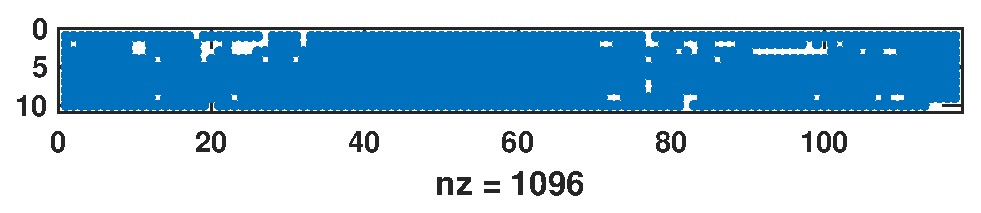
\includegraphics[width=0.8\textwidth]{original_papers/icassp_2018/figs/bat_20180710_inl.eps} \\
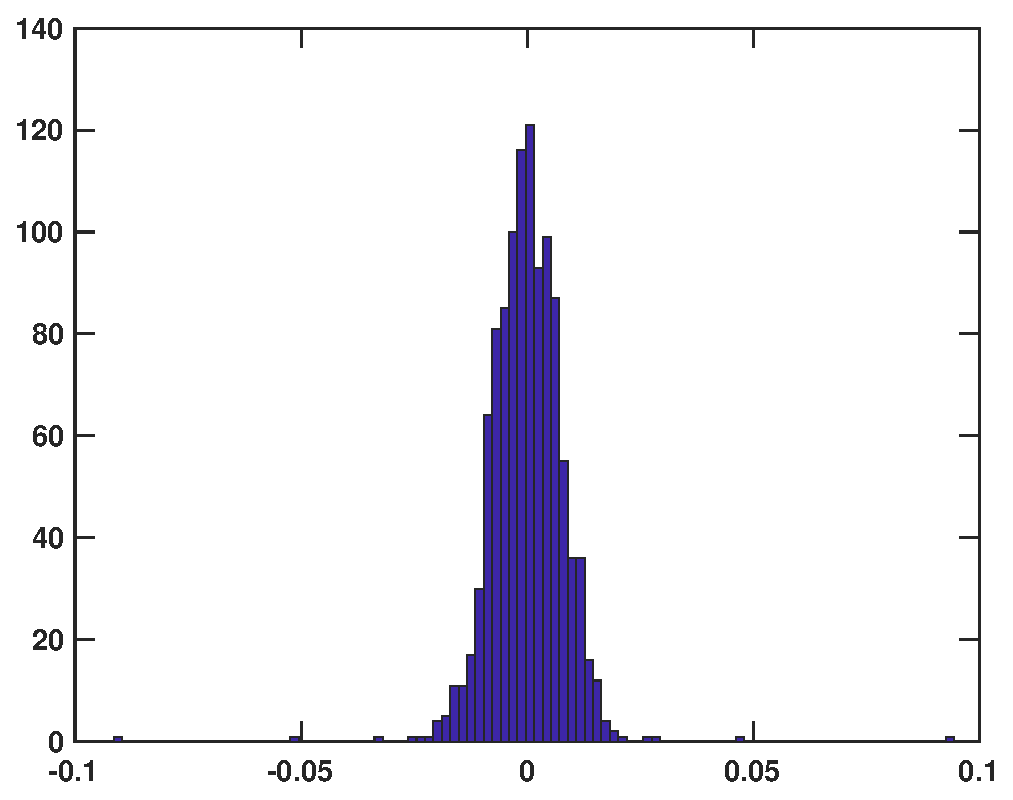
\includegraphics[width=0.4\textwidth]{original_papers/icassp_2018/figs/bat_20180710_res.eps} 
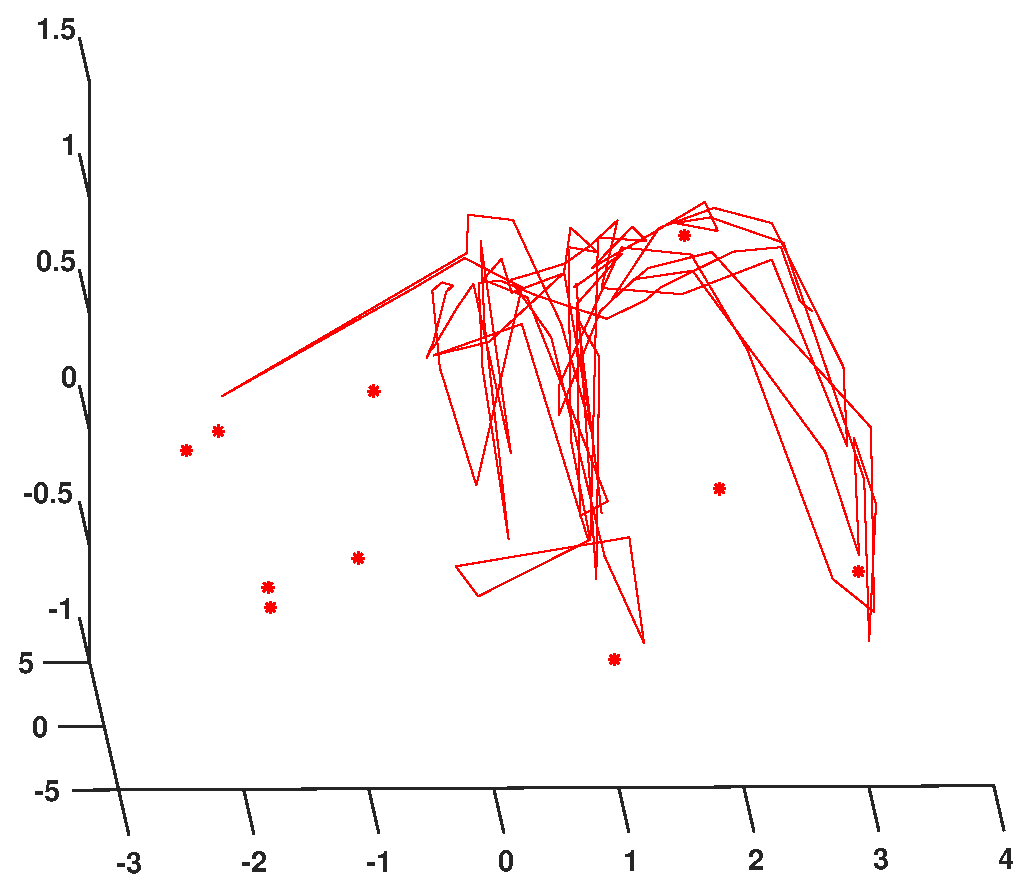
\includegraphics[width=0.4\textwidth]{original_papers/icassp_2018/figs/bat_20180710_fig.eps} \\
\end{tabular}
\caption{For the cave experiment the figure shows detected inliers $\Win$ (top), inlier residual histogram (bottom left) and  estimated microphone and sound source positions, red dots and line respectively (bottom right).}
\label{f_bat}
\end{figure}

\vspace{-5pt}
\section{Conclusions}
\label{sec:exp}
\vspace{-5pt}

In this paper, a novel method has been constructed to efficiently solve a TDOA problem with a constant offset. This has been verified using simulated data to test the solver and real experimental data to test our algorithms in realistic scenarios.

Looking at Figure \ref{fig:f_hist} and Table \ref{Tabletime}, it can be seen that the calculation of the offsets and the calculation of the relaxed form \(\theta_2\) are very fast solvers without loss in numerical accuracy. The advantage of this is that when using a RANSAC approach, the iterations are performed quickly, giving a good initial estimate in which to optimize over, which is important in highly
non-linear systems such as this.

Looking at the results from the office experiment, Figure \ref{f_454H}, we can see that the calculated microphone positions are accurate and the residuals are small, mostly in the range \(\pm 0.04~m\). Further to this our inlier set appears to be accurate. The first and last few columns (corresponding to sound emissions) are not used in our initialisation. This is correct because the recording started before the chirps were sounded and ended after, so the chirp detection algorithm falsely determined that they were also chirps but our method decided that the data in those regions do not fit the model. A comparison of the calculated microphone positions were made to a solution from a Full TDOA system, (\cite{kuang2013stratified}), which produced similar results and very similar residuals. This provided a sanity check that the chirp detection was working correctly and that from this dataset a better solution could not be found.

For the cave experiment, similar conclusions can be made, since the residuals are very low, we can conclude that we have an accurate model. This gives a real life example of how algorithms such as the one proposed can be used.

For future work, the study of the number of inliers could be of use. At the moment our algorithm may not extend to more rows and columns if the initial solution is poor, perturbing our final solution. Perhaps a method which could adapt the initial selection in order to give a required amount of inliers could be more advantageous.

\hypertarget{tacost-testing-and-simulating-the-performance-of-acoustic-tracking-systems}{%
\chapter{\texorpdfstring{\texttt{tacost}: Testing and simulating the performance of acoustic tracking systems}{tacost: Testing and simulating the performance of acoustic tracking systems}}\label{tacost-testing-and-simulating-the-performance-of-acoustic-tracking-systems}}

\chaptermark{simulating performance of acoustic tracking}

This chapter was published as a preprint on \emph{biorXiv}:

\emph{Beleyur, T. (2020). \texttt{tacost}: Testing and simulating the performance of acoustic tracking systems. bioRxiv.}

\newpage

\hypertarget{tacostabstract}{%
\section*{Abstract}\label{tacostabstract}}
\addcontentsline{toc}{section}{Abstract}

\texttt{tacost} is a Python package to allow the testing of acoustic tracking systems. While many microphone array systems have been characterised analytically and experimentally - these are time-intensive methods. \texttt{tacost} provides a simulation based framework to rapidly assess the tracking behaviour of multiple array geometries, and the dissection of other relevant parameters. This paper explains briefly the design of the package and highlights two example use cases in which the tracking accuracy of different microphone geometries are characterised.

\newpage

\hypertarget{introduction}{%
\section{Introduction}\label{introduction}}

Acoustic tracking is a common method used to study vocalising animals such as birds, bats and cetaceans \citep{suzuki2017harkbird, aubauer1996acoustical, mohl2000sperm, Hugel2017, Holderied20032293, rhinehart2020a, blumstein2011a}.
Using acoustic tracking, biologists can detect the position of the animal and track it through space as it moves over time. The localisation accuracy of an acoustic tracking system depends on a variety of factors. There are \emph{internal} factors such as microphone array geometry, signal processing routines, and the mathematical formulations used to localise sounds (time-of-arrival, time-of-arrival-difference, angle-of-arrival, power-steering). The \emph{external} factors include aspects related to the actual signal itself, ie. signal-to-noise ratio, and spectro-temporal properties of the emitted sound (noise, linear/hyperbolic sweep) \citep{Wahlberg1999}.
While experiments and analytical modelling may be the definitive way to determine a tracking system's end accuracy, simulations allow a quick and systematic method to estimate the source of tracking errors. \texttt{tacost} provides a flexible workflow to manipulate and study the effect of both internal and external factors. \texttt{tacost} generates audio files for source positions and array geometries specified by the user. This allows the user to analyse the efficacy of their tracking system's baseline performance.

\hypertarget{statement-of-need}{%
\section{Statement of need}\label{statement-of-need}}

Generating simulated audio for a set of source sounds, positions and a given array configuration is a relatively simple task. However, to my knowledge, there are no publicly available, tested and documented packages for this task published to date. Codebases that are publicly available have the advantage of being used by a larger user-base and can thus benefit from bug discoveries much faster than in-house or individually written one-time use scripts. \texttt{tacost} provides a robust and well-documented software workflow \citep{Taschuk2016} with user and developer friendly documentation \href{https://tacost.readthedocs.io/en/latest/}{hosted online}. \texttt{tacost} contributes to the Python scientific ecosystem in the hope of promoting the growth of acoustics and bioacoustic research in open-source languages like Python. In particular, \texttt{tacost} will help researchers working in the field of acoustics and bio-acoustics \citep[eg.][]{deframond2020} plan and examine the behaviour of their acoustic tracking systems.

\hypertarget{design}{%
\section{Design}\label{design}}

The design of \texttt{tacost} focusses on a reproducible and user-friendly method \citep{Wilson2012} to generate WAV files that form the input for acoustic tracking softwares. Users may interact with \texttt{tacost} through custom-written Python scripts
by calling it as a Python package with \texttt{import\ tacost} or in the `no-coding' mode. The `no-coding' mode is especially suitable for users unfamiliar with Python. The no-coding mode is based around a parameter file that is used to specify various parts of the WAV file to be created.
Through the parameter file the user can specify the emitted sound, source positions, inter-sound-intervals, sampling rate and other relevant variables to customise the test scenario.

\hypertarget{examples}{%
\section{Examples}\label{examples}}

The localisation accuracy of a microphone array may not be uniform over 3D space \citep{aubauer1996acoustical, Wahlberg1999}. This accuracy is independent of the actual signal and recording conditions of the input data, but rather dependent on the array geometry and mathematical formulations used to record and calculate sound source position.

The accuracy of a few microphone array configurations has been characterised analytically \citep{aubauer1996acoustical} and experimentally \citep{Wahlberg1999}. While reflecting the system's capabilities, analytical
and experimental characterisations are often time-intensive. In contrast, simulation uncovers the intrinsic accuracy of an array relatively quickly through the use of audio files with simulated emission points spread across the recording volume of interest.
\texttt{tacost} can be used to characterise the maximal localisation accuracy of an acoustic tracking system with novel array geometries and recording scenarios. In Example 1, I show how \texttt{tacost} can be used to verify known trends in
localisation error with the tristar60, a commonly used array system. In Example 2, I show how \texttt{tacost} can be used to estimate the expected localisation error in a multi-microphone array with a novel and field-friendly geometry.

\hypertarget{localisation-accuracy-of-the-tristar60-system}{%
\subsection{Localisation accuracy of the tristar60 system}\label{localisation-accuracy-of-the-tristar60-system}}

The tristar60 array is a commonly used array geometry \citep{aubauer1996acoustical, Holderied20032293, Hugel2017, Lewanzik2018} with 4 microphones in a plane on an inverted T array. Three peripheral microphones are placed 120\(^{\circ}\) to each other at 60 cm radial distance from the central mic on the inverted T-array.

A series of emission points spanning the upper right quadrant of the array were simulated. The emitted sound was set to a linear sweep. The output WAV files from \texttt{tacost} were run through the TOADSuite package \citep{holger_toadsuite_manual, toadsuite_peterstilz}, a software package that localises sounds using the time-of-arrival-differences across channels. Figure \ref{tacostfig1} shows the localisation accuracy map
for the tristar60 microphone array. It can be seen (Figure \ref{tacostfig1}) that localisation error increases with increasing radial distance from the central microphone, and remains \textless7\(\%\) of the radial distance.

\begin{figure}
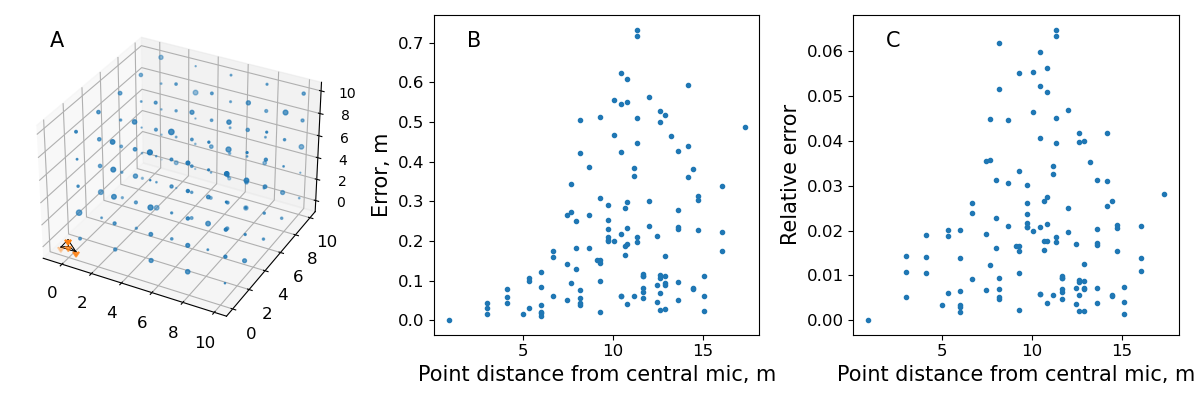
\includegraphics[width=1.0\columnwidth]{original_papers/tacost/data_for_figures/analysis/fig1_points_and_error.png}
\centering
\caption{Accuracy of a sound source localisation based on time-of-arrival-differences with a tristar60 array. A) The tristar60 microphone array is placed at the origin of the coordinate system (bottom left, orange dots connected by black lines). The blue points are the simulated source positions which form a 'calibration grid'. The size of each dot is proportional to the localisation error B) The localisation error increases with increasing radial distance of source from the central microphone. The error is the euclidean distance between the predicted and simulated source point.The errors range between 0-0.7m. C) The relative error of localisation, defined as $\frac{Localisation \:error}{Distance \:from \:central \:microphone}$. Even though absolute localisation error tends to increase with distance from array, all localisation happens with <7 $\%$ relative error.}
\label{tacostfig1}
\end{figure}

\hypertarget{localisation-accuracy-of-a-multi-microphone-array-in-the-field}{%
\subsection{Localisation accuracy of a multi-microphone array in the field}\label{localisation-accuracy-of-a-multi-microphone-array-in-the-field}}

While recording in the field, it may be difficult to use fixed arrays mounted on stands. Arrays on stands are difficult to carry and may also influence the behaviour of the animals being recorded. It is thus advantageous to use less obtrusive microphone geometries, for instance by placing microphones are placed on pre-existing structures such as the walls of a cave or trees. These microphone geometries are field-friendly, but their localisation accuracy is hard to characterise analytically. \texttt{tacost} is an ideal tool to explore the tracking performance of such flexibly placed microphone arrays.

(Figure \ref{tacostfig2}A) shows the microphone array geometry and recording system described in \citep{Batstone2019}. In short, the array consisted of 11 microphones, 4 of them on a 120cm tristar, and the remaining 7 microphones attached to the walls of a cave. A series of sound emission points were created simulating points in the volume enclosed by the array. The points matched the volume echolocating bats flew within. The simulated sound was set to a linear sweep, which mimicked that of a bat call. The \texttt{tacost} output WAV files were analysed with the TOADSuite. The resulting accuracy map reveals that overall, the localisation error is between 7-30 centimetres for the given emission points. This corresponds to a maximum error of upto 30cm in tracking the position, and of upto 19\(\%\) relative error. In contrast to the previous example highlighting the increase in tracking error with increasing source sound distance, these results show a somewhat different trend. The relative error is also much higher, and it may have to do with the positioning of the sound sources in the volume with reference to the array. The relative location of the sound source affects the tracking accuracy \citep{aubauer1996acoustical}.

\begin{figure}
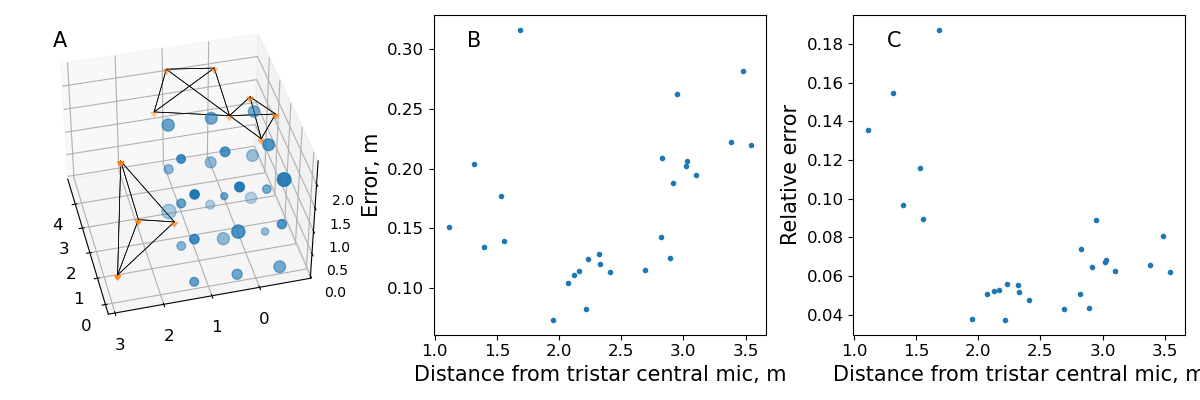
\includegraphics[width=1.0\columnwidth]{original_papers/tacost/data_for_figures/analysis/fig2_points_and_error.png}
\centering
\caption{Localisation accuracy of a multi-microphone array in the field, localised with time-of-arrival-differences. A) The line-connected points (orange) represent the microphone array consisting of 11 microphones. Four microphones are in a tristar 120 array (left, tristar array with 120cm radial distance from central mic), and 
the remaining 7 mics are placed on the walls of the cave (top right, two quadirlateral outlines joined at a common vertex represent the 7 mics on the cave walls). The free-standing points (blue) are  the simulated emission points which form a 'calibration grid'. Each simulated point is shown as a dot, and the size of the dot is proportional to the tracking error. B) The distribution of localisation error. The error is 
the euclidean distance between the predicted and simulated point. The localisation error is between 0.07-0.32 m for the given points. C) The relative localisation error with reference to the central mic of the 120 cm tristar array microphone. The 95$\%$ile bounds of tracking error lie between 3.7-16.6$\%$, with a maximum of 18.8$\%$ error. Even points that are nearby seem to be localised with a higher relative error. This higher relative error may be the result of sound source position with reference to the microphone array.}
\label{tacostfig2}
\end{figure}

\hypertarget{future-directions}{%
\section{Future directions}\label{future-directions}}

\texttt{tacost} as it stands is currently written to implement a first-order assessment of a tracking system's accuracy. The package has been primarily written keeping acoustic signals propagating through air where the velocity of sound is assumed to be constant. It may also be used to test tracking in radar or underwater sonar systems, contingent on how uniform the medium of wave propagation is over the distances being studied. As of version 0.1.0
,straight line propagation of signals are simulated, without spherical spreading or atmospheric absorption implemented. Future releases may include such propagation losses. Another important aspect affecting all tracking systems is the directionality of the sensors (microphones) and emitted signals (animal vocalisations, calibration speakers). A common problem in acoustic tracking with bats and cetaceans is not being able to track animals because their echolocation calls can be very directional \citep{Matsuta2013, Surlykke2012, Koblitz2016}. Implementing sensor and source sound directionality will help assessing how many microphones might be required to successfully track animals in their surroundings, and which array geometries are best able to do so.

\hypertarget{acknowledgements}{%
\section{Acknowledgements}\label{acknowledgements}}

This work was supported by a doctoral fellowship from the German Academic Exchange Service (DAAD) and the International Max Planck Research School for Organismal Biology.
I would like to thank Léna de Framond for generating the acoustic localisation output, Holger R Goerlitz for helpful comments on this manuscript and discussions on the topic of tracking, and the IT team atthe Max-Planck Institute for Ornithology for their support.

\hypertarget{itsfm}{%
\chapter{itsfm}\label{itsfm}}

Some \emph{significant} applications are demonstrated in this chapter.

\hypertarget{example-one}{%
\section{Example one}\label{example-one}}

\hypertarget{example-two}{%
\section{Example two}\label{example-two}}

\hypertarget{general-discussion}{%
\chapter{General Discussion}\label{general-discussion}}

The part where things get concluded.The part where things get concluded.The part where things get concluded.The part where things get concluded.The part where things get concluded.The part where things get concluded.The part where things get concluded.The part where things get concluded.The part where things get concluded.The part where things get concluded.The part where things get concluded.The part where things get concluded.The part where things get concluded.The part where things get concluded.The part where things get concluded.The part where things get concluded.The part where things get concluded.The part where things get concluded.The part where things get concluded.The part where things get concluded.

\hypertarget{acknowledgements}{%
\chapter{Acknowledgements}\label{acknowledgements}}

\emph{``There was a bat bat bat bat bat bat bat bat bat bat bat,
\newline
There was a wizard wizard wizard wizard wizard wizard wizard wizard wizard,
\newline 
There was a guy guy guy guy guy guy guy guy guy guy guy,
\newline
They worked by a lake with many swans
\newline
Studying bats from dusk to dawn\ldots.''}
- \emph{There was a bat bat bat bat bat bat bat bat bat bat bat}, Thejasvi Beleyur, performed 2019 MPIO Open Doors Science daything???

IMPRS for Organismal Biology
Neetash for playing the multiple roles of friend, colleague and wife over the past few years.
All current and past members of the Acoustic and Functional Ecology group for a great working environment. Office mates Daniel and Theresa.

Apurva-Sindhu, Deepu-Ravi - my family in Germany for creating a home away from home over the past many years with their hospitality, food and love!!

My parents, for constantly supporting all my weird ideas of becoming, at various points, a vet, a `zoologist' (even before I actually knew what the word meant), a musician, and now this! I am definitely nowhere close to where I started, but am quite happy with whatever my current profession is called!

Reni for providing an oasis to retreat from work and and Dieter for being the amazing conversationalist and story-teller he is. Their amazing company.

And finally, I would not be here without all the bats flying through the night. All the bats that hung around as I fumbled with cables with numb hands on cold autumn nights, as I learnt to patiently deal with (hundreds of?) metres of tangled cable every night, and set up equipment hoping they'd land up. When they did it was always a pleasure to watch and hear them. So here's to all you hovercraft Daubis, hyper pipistrelles and gliding Mouse-eared bats, none of this would have been possible without all of you!

\hypertarget{author-contributions}{%
\chapter{Author contributions}\label{author-contributions}}

Chapter 2:

Chapter 3:

Chapter 4:

Chapter 5:

Chapter 6:

  \bibliography{beleyur-goerlitz-2020-refs.bib,tacost-references.bib,cotdoa-filtered.bib,intro-discussion-refs.bib}

\end{document}
